\documentclass[11pt,a4paper,titlepage,oneside]{report}

\usepackage[english]{babel}
\usepackage[utf8]{inputenc} % input encoding is UTF-8

\usepackage[table,xcdraw]{xcolor}
\usepackage{graphicx}
\usepackage{tabularx}
\usepackage{subcaption}
\usepackage{color}
\usepackage[unicode,pdftex]{hyperref}
\usepackage{xcolor}
\usepackage{longtable}
\usepackage{listings}
\usepackage{amsmath}
\usepackage{pdfpages}
\usepackage[acronym,numberedsection=autolabel]{glossaries}

\usepackage{listings}
\usepackage{color}

\definecolor{dkgreen}{rgb}{0,0.6,0}
\definecolor{gray}{rgb}{0.5,0.5,0.5}
\definecolor{mauve}{rgb}{0.58,0,0.82}

\lstset{frame=tb,
  language=Bash,
  aboveskip=3mm,
  belowskip=3mm,
  showstringspaces=false,
  columns=flexible,
  basicstyle={\small\ttfamily},
  numbers=none,
  numberstyle=\tiny\color{gray},
  keywordstyle=\color{blue},
  commentstyle=\color{dkgreen},
  stringstyle=\color{mauve},
  breaklines=true,
  breakatwhitespace=true,
  tabsize=3
}

\makeglossaries

\newacronym{netcdf}{NetCDF}{NETwork Common Data Form}
\newacronym{NTNU}{NTNU}{the Norwegian University of Science and Technology}
\newacronym{QA}{QA}{Quality Assurance}
\newacronym{L}{L}{Low}
\newacronym{M}{M}{Medium}
\newacronym{H}{H}{High}
\newacronym{HTML}{HTML}{HyperText Markup Language}
\newacronym{HTML5}{HTML5}{HyperText Markup Language version 5}
\newacronym{CSS}{CSS}{Cascading Style Sheets}
\newacronym{EDGE}{EDGE}{Enhanced Data rates for GSM Evolution}
\newacronym{PNG}{PNG}{Portable Network Graphics}
\newacronym{MEOPAR}{MEOPAR}{Marine Environmental Observation Prediction and Response Network}
\newacronym{WMS}{WMS}{Web Map Service}
\newacronym{THREDDS}{THREDDS}{Thematic Realtime Environmental Distributed Data Services}
\newacronym{OPENDAP}{OPeNDAP}{Open-source Project for a Network Data Access Protocol}
\newacronym{OGC}{OGC}{Open Geospatial Consortium}
\newacronym{WCS}{WCS}{Web Coverage Service}
\newacronym{HTTP}{HTTP}{HyperText Transfer Protocol}
\newacronym{NCML}{NcML}{\gls{netcdf} Markup Language}
\newacronym{XML}{XML}{Extensible Markup Language}
\newacronym{TDS}{TDS}{\gls{THREDDS} Data Server}
\newacronym{SSD}{SSD}{Solid State Drive}
\newacronym{NCWMS}{ncWMS}{NNN}
\newacronym{BSD}{BSD}{Berkeley Software Distribution}
\newacronym{JPEG}{JPEG}{Joint Photographic Experts Group}
\newacronym{GIF}{GIF}{Graphics Interchange Format}
\newacronym{CPU}{CPU}{Central Processing Unit}
\newacronym{TMS}{TMS}{Tile Map Service}
\newacronym{URL}{URL}{Uniform Resource Locator}
\newacronym{WMTS}{WMTS}{Web Map Tile Service}
\newacronym{WMSC}{WMSC}{Web Map Server Tile Cache}
\newacronym{GUI}{GUI}{Graphical User Interface}
\newacronym{API}{API}{Application Programming Interface}
\newacronym{JSON}{JSON}{JavaScript Object Notation}
\newacronym{Fimex}{Fimex}{File Interpolation, Manipulation and EXtraction}
\newacronym{PSP}{PSP}{Polar Stereographic Projection}


\newglossaryentry{pre-study}{name=pre-study, description={is a document produced before the implementation phase, which informs the customer of possible solutions to their problem}}
\newglossaryentry{pre-delivery}{name=pre-delivery, description={is a preliminary delivery of the main report, that is meant to give the external examiner an introduction to the groups work}}
\newglossaryentry{front-end}{name=front-end, description={is the name given to the part of software that the user interacts with}}
\newglossaryentry{back-end}{name=back-end, description={is the name given to the part of software the user does not interact with, and that performs a specialized task.}}
\newglossaryentry{course compendium}{name=course compendium, description={is a document given to the students, which outlines the course, describes the rules and expectations for the groups work, and gives the structure and content of the final report}}
\newglossaryentry{protocol}{name=protocol, description={is a set of predefined rules of conduct and procedures. In computer science, it often describes the rules for communication between two parts}}
\newglossaryentry{open source}{name=open source, description={is software where the source code is available to everyone, and anyone can alter and share the code}}
\newglossaryentry{prototype}{name=prototype, description={is an early version of something, meant to test specific features}}
\newglossaryentry{proof of concept}{name=proof of concept, description={is a system that proves the feasibility of an idea. It is usually not usable as part of a final system, but rather built as proof of an idea.}}

\begin{document}



% Title page %%%%%%%%%%%%%%%%%%%%%%%%%%%%%%%%%%%%%%%%%%%%%%%%%%%%%%%%
\begin{titlepage}

\begin{figure}
\centering
\begin{subfigure}{.5\textwidth}
\centering

\includegraphics[width=0.8\textwidth]{img/logo_NTNU.png}\\
\end{subfigure}%
\begin{subfigure}{.5\textwidth}
\centering

\includegraphics[width=0.8\textwidth]{img/logo_SINTEF.jpg}
\end{subfigure}
\end{figure}

\begin{center}
{\LARGE \textbf{TDT4290 - Customer Driven Project}}
\vfill
{\Huge \textbf{Ocean forecast}}

\vspace{12pt}
{\LARGE \textbf{SINTEF}}

\vspace{30pt}
{\LARGE \textbf{Final report}}
\vfill
{\LARGE \textbf{Autumn 2014}}
\end{center}
\vfill
\begin{tabular*}{\textwidth}{@{\extracolsep{\fill}} l l}
\textbf{Group 6} & \textbf{Advisor} \\
Arve Nygård & Gleb Sizov \\
Anders Smedegaard Pedersen & \\
Emil Jakobus Schroeder & \\
Hans Kristian Henriksen & \\
Marco Radavelli & \\
Ondrej Hujnak & \\
Ruben Håskjold Fagerli & \\
\end{tabular*}

\end{titlepage}

% Empty page %%%%%%%%%%%%%%%%%%%%%%%%%%%%%%%%%%%%%%%%%%%%%%%%%%%%%%%%
\newpage
\thispagestyle{empty}
\mbox{}
\newpage

% Abstract %%%%%%%%%%%%%%%%%%%%%%%%%%%%%%%%%%%%%%%%%%%%%%%%%%%%%%%%%%
\begin{abstract}
In the choice of location, as well as in the daily operations of fish farms, both historical data and up to date projections on sea currents are vital. SINTEF has given the task of visualizing data on ocean currents, temperature, salinity and other variables in areas around fish farms, to be used by stakeholders in the sea farming industry. 

Our group of seven students have used the fall semester at the Norwegian University of Science and Technology to do a full scale software development process in order to solve this task.

The group has written a pre study, were systems that are currently in use have been investigated, and technologies that could be used for custom built solutions have been evaluated. Using the Scrum methodology, the group has worked to develop both a front and back end \gls{prototype} of such a system.

The \gls{prototype} developed is able to read NetCDF files from SINTEFs simulations, and visualize this dynamically at the users discretion. This includes handling files that overlap both in area and resolution. 

Although the solution is a \gls{prototype}, and not ready for full scale deployment, it proves that developing a custom system is within reach, and should be considered.

\end{abstract}

% Signatures %%%%%%%%%%%%%%%%%%%%%%%%%%%%%%%%%%%%%%%%%%%%%%%%%%%%%%%%
\thispagestyle{empty}
\begin{center}
{\large \textbf{Trondheim, \today}}\\
\vspace{2.5cm}
\begin{tabularx}{\textwidth}{@{\extracolsep{1cm}} X X }
\dotfill & \dotfill \\
~Arve Nygård & ~Anders Smedegaard Pedersen \\[1cm]
\dotfill & \dotfill \\
~Emil Jakobus Schroeder & ~Hans Kristian Henriksen \\[1cm]
\dotfill & \dotfill \\
~Marco Radavelli & ~Ondrej Hujnak \\[1cm]
\dotfill & \\
~Ruben Håskjold Fagerli & \\[1cm]
\end{tabularx}
\end{center}

% Table of contents %%%%%%%%%%%%%%%%%%%%%%%%%%%%%%%%%%%%%%%%%%%%%%%%%
\tableofcontents
\addtocontents{toc}{\protect\thispagestyle{empty}}

% List of figures %%%%%%%%%%%%%%%%%%%%%%%%%%%%%%%%%%%%%%%%%%%%%%%%%%%
\listoffigures
\addtocontents{lof}{\protect\thispagestyle{empty}}

% List of tables %%%%%%%%%%%%%%%%%%%%%%%%%%%%%%%%%%%%%%%%%%%%%%%%%%%%
\listoftables
\addtocontents{lot}{\protect\thispagestyle{empty}}

\pagenumbering{arabic}
\setcounter{page}{0}

% Main body %%%%%%%%%%%%%%%%%%%%%%%%%%%%%%%%%%%%%%%%%%%%%%%%%%%%%%%%%
%%%%%%%%%%%%%%%%%%%%%%%%%%%%%%%%%%%%%%%%%%%%%%%%%%%%%%%%%%%%%%%%%%%%%

\chapter{Introduction}
\section{TDT 4290 - Customer driven project}
The task is set forth in the subject TDT 4290 - Customer driven project at \gls{NTNU}. The goal of the course is 
\begin{quote}
(...)to give the students a practical experience of carrying out all the phases of a typical customer guided IS/IT-project. \cite{TDT4290:Intro}
\end{quote}
The subject divides the students into random groups, and assigns each group an assignment. The assignments are real problems that businesses needs solved. 

Although the assignment is to follow the entire process of an IT-project, the focus is on the earlier phases of a project. Thus, an important part of the assignment is the work leading up to the implementation phase. There is obviously also an important focus on the implementation itself. Maintenance is however left out of the scope of the projects.

\section{Customer}
The customer is SINTEF Fisheries and Aquaculture (SINTEF Fiskeri og havbruk AS). 
SINTEF was founded in 1950 and it is nowadays organized into 8 divisions. The division of Fisheries and Aquaculture was founded in 1999 and represents technological expertise and industry knowledge in the utilization of renewable marine resources. Under the vision "Technology for a better society" it works for a knowledge-based bio marine industry. Its goal is to meet market demands for technological research and development on renewable marine resources.

\section{Ocean currents}
The study of ocean currents allows for predicting what conditions can be expected in an area, both in short and long term. Historical data can be used to asses how an area will be exposed to temperature and salinity changes. Up to date projections are crucial for day to day operations like feeding and lice removal. It can also be used to predict the spreading of lice from one farm to another.

This makes the most relevant users of the system fish farmers, either in the planning or operation phase of the farm. The system is also relevant to anyone conducting ocean research in the given areas, and other stakeholders that can use information on the condition of the sea in their work.

\section{Assignment and scope}
The client, SINTEF Fisheries and Aquaculture, has given us the project labeled "Ocean Forecast". The task is to improve SINTEFs existing system of storing and retrieving data, as well as the way the data is presented to the end user. 

In agreement with the customer, the group has defined the following scope of the assignment:

\begin{quote}
Make a \gls{pre-study} that examines what technology can be used to replace the current collection of PDFs, and instead serve the end user with custom visualizations on a web page. Follow the study with an implementation of a \gls{proof of concept} system that is able to read from a collection of \gls{netcdf}-file, and present data to the end user based on custom chosen variables. We will ignore any bottlenecks that may exist in SINTEFs systems, and assume that they are fixable. Our end report will contain suggestions for further development and analysis.
\end{quote}

\section{Group resources}
\label{sec:GroupResources}
The group consists of seven people with diverse skills. In the starting phase of the project, the group assessed the different skills, and used this to distribute tasks, and areas of responsibilities. 

The project is set to run from August 28th until November 20th, for a total of 85 days, or 12 weeks and 1 day. As with all subjects given at \gls{NTNU}, a student is expected to work 12 hours for every 7,5 study points. For this course, this amounts to 24 hours of work every week. Due to the fact that the presentation is given the week before the end of the semester, the \gls{course compendium} sets the required work load to 25 hours a week. 

For our group, this amounts to about 2100 work hours in total. Every week, the group has 6 hours of meeting time, and is required to hand in documents for the advisor meeting. An estimate of 4 hours is given for the production of these documents. Given this, approximately 1550 hours can be dedicated to solving the customers problem.

\begin{equation}
Total\:work\:hours = 25\:\frac{hours}{week} * 12\:weeks * 7\:people = \underline{\underline{2100\:hours}} \nonumber
\end{equation}

\begin{equation}
\begin{split}
Meetings\:and\:documents = (6\:hours\:of\:meetings * 12\:weeks * 7\:people) + \\ 
(4\:hours\:for\:documents * 12\:weeks) = \underline{\underline{552\:hours}} \nonumber
\end{split}
\end{equation}

\begin{equation}
Time\:for\:product = 2100\:hours - 552\:hours = \underline{\underline{1548\:hours}} \nonumber
\end{equation}

Group members are free to distribute the workload as they see fit, and according to their lecture schedule. The only requirement is that deadlines are met, and that the group members participate in all meetings. 

\chapter{Planning}
Before starting a project of this scale, a lot of planning has to be done. How will development be done, who will be responsible for what, which risks should be planed for, and so on. This chapter will give an overview of the planning done before the project was started. 

\section{Project stakeholders}
The stakeholders of this project are the following:
\begin{description}
\item[Project owner] SINTEF Fisheries and Aquaculture
\item[Supervisor] Gleb Sizov
\item[Examiner] 
\item[Team members] 
\end{description}

\section{Background for the project: software system development}
The customer owns a working solution, running on its own servers, for the delivery and analysis of  tracked and predicted marine data. The data is stored in a special format, \gls{netcdf}, designed to be self-describing, scalable and appendable \cite{netCDF:factsheet}.
The background for this project is to optimize the current, slow and memory-consuming solution. In the project description, the customer asks the group to either develop a new back end system, or produce a new front end for the current system. 

\section{Measurement of project effects}
Some predefined criteria must be met in order to consider the project to have been successful. The product must be working according to the requirements, and pass all tests. All requirements prioritized high and medium must be fulfilled. Requirements that have low priority are viewed as nice to have, but should be implemented if there is sufficient time.
In this project, quite open goals were set by the customer, and no precisely quantifiable measurements were defined. This makes the approval of the project subjective, and the group will have to keep the customer closely involved, to ensure continuous feedback.

If working on improving the actual solution the measurements should be:
\begin{itemize}
\item The time it takes to visualize data for the end user should be "reasonably low" even with slow internet connection (like from Chile) or from a mobile device
\item The same displayed features as the actual working system are still available
\end{itemize}

If working on new use cases, the measurements should be:
\begin{itemize}
\item The same displayed features as the actual working system are still available
\item New features (such as mobile app and new charts) are added in order to cover more use-cases 
\end{itemize}
In both cases, an open source based solution is considered to be better than a commercial one.

\section{Life cycle model}
\label{sec:Scrum}
The group has chosen to use the Scrum methodology for the project. This is an agile method that focuses on incremental development. The customer is heavily involved in the development process, and is given frequent updates and demos of the progress of the team. 

\subsection{Scrum cycle}
\begin{figure}[h]
\begin{center}
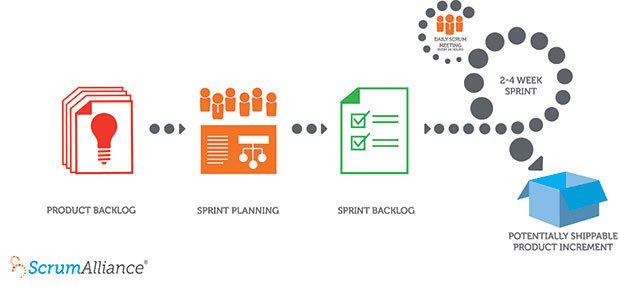
\includegraphics[height=150px,width=340px]{img/Scrum.jpg}
\caption{Scrum cycle}\cite{ScrumCycle}
\label{fig:gantt}
\medskip
\small
\end{center}
\end{figure}

In the scrum methodology, there is a set way to conduct a development process. The process starts by laying out a product backlog. This is a overview of what needs to be done to complete the entire product. It does not have to have very high detail, but it should be detailed enough to give a clear idea of how the team should proceed. 

After the product backlog is written, the first sprint is planned. In this planning meeting, the team estimates the time needed for each task, and takes on the tasks needed to complete the goal set for the sprint. This process is done in cooperation with the customer. The customer may set the sprint goal, or get more directly involved in the selection of tasks. 

When the team has chosen the tasks to be completed, the sprint is locked, and new tasks may not be added by the customer. This gives the development team a noise free environment, and allows them to focus on the task ahead. 

In the sprint cycle, which typically lasts for around 3 weeks, the team has daily meetings to update on progress and challenges. This meeting is lead by the scrum master. The daily meeting is known as a standup, as the participants are expected to stand during the meeting. Every person is given about two minutes to give an update of their work. This update should answer three questions:

\begin{itemize}
\item What did I do yesterday?
\item What am i going to do today?
\item Are there any problems that can obstruct my progress?
\end {itemize} 

When the sprint is completed, the customer is given a demo of what the team has completed. This should be all that was agreed on in the sprint planing meeting. The customer is now free to give new priorities to items in the product backlog before the team picks new tasks for the next sprint. 

After the sprint, the team should conduct a retrospective. In the retrospective, the team members are to discuss the sprint that is just concluded, and list experiences into one of three categories:

\begin{itemize}
\item Things we should continue doing
\item Things we should stop doing
\item Things we should start doing
\end {itemize} 

This is a process that is usually conducted together with the customer, as the customer can add valuable insight into the teams work from a business perspective. The goal of the retrospective is for the team to identify what helps them in their work, and what is hindering them. This way, it is possible to make changes that positively effects the team.

\subsection{Scrum adaptions}
\label{subsec:scrumadaptations}
As our development project is part of a university course that runs in parallel with other subjects, it is impossible to follow the standard scrum process. Given this, the group made some choices that diverges from the standard scrum methodology.

\begin{itemize}
\item Meetings are not conducted every day, but rather twice a week. This fits better with the schedule of the group members, and takes into consideration that there is no demand for work to be done every day. 
\item Sprint length has been chosen as one week. This is short compared to the Scrum standard, but it provides the group with a motivational pressure, as well as making the sprints easier to estimate. 
\item Product demos are set to every other week. This means that there will be sprints that are not presented to the customer. In choosing this, the group is able to have sprints that focus on the internal demands set forth by \gls{NTNU}, as well as making more progress between customer meetings.
\item Retrospectives at the end of each sprint would mean setting aside around 50-70 hours of work time for retrospectives. As the group is only in a position to change their own work habits, and can not make changes to the course, nor to the general work process of the customer, it was decided that retrospectives will be dropped. In addition, the customer will probably not be able to be present at retrospectives, lowering their value. Instead, team meetings and advisor meetings will take the place of retrospectives. 
\item The scrum master is usually responsible for shielding the development team from the outside world. In this subject, it will not be possible to do this, as group members are required to attend advisor meetings and customer meetings. Thus, the scrum master will be more of a project manager, responsible for the teams progress and efforts. 
\end {itemize}

These changes make the Scrum method well suited for use in the project. Although it is important to try to follow well tested methodologies to the letter, one can not allow them to block progress, or disturb the workflow of the team. When in a special work situation, as the group is in, this type of adaptions are necessary for the efficient use of any development methodology. 

\subsection{Other alternatives}
While it was early clear that the team wanted to work in a scrum-like manner, other methodologies of development could also have been used, and was discussed. In particular, Kanban and waterfall with feedback.

\paragraph{Kanban}
While Scrum is driven by estimations, and motivates by limiting the amount of time for each sprint, Kanban attempts to motivate by limiting the amount of concurrent tasks the team is allowed to have. For example, the team can set a limit of 4 tasks in development, 3 in \gls{QA} and 2 in test. This way, the team is motivated to finish tasks, as it will free up space for new tasks. 

As none in the team is particularly proficient in Kanban, and most of the team has some knowledge of Scrum, Kanban did not seem like a wise choice. The biggest factor in not choosing Kanban was the fear of having to use a lot of time learning the methodology, and thus have less time left for the actual development. 

\paragraph{Waterfall with feedback}
The waterfall methodology is one of the oldest development methodologies, and is usually viewed as a rigid, one way process. Every step must be completed before moving to the next. This means that the customer must clearly specify what they want before any development can start. This made the team reject the traditional waterfall model, as the customer is not clear on what they want.

An adaptation to the waterfall model is the waterfall model with feedback. This model follows the traditional waterfall methodology, but allows the team to move back to a previous phase when needed. It is further illustrated in figure \ref{fig:WaterfallFeedback}.

\begin{figure}[h]
\begin{center}
\fbox{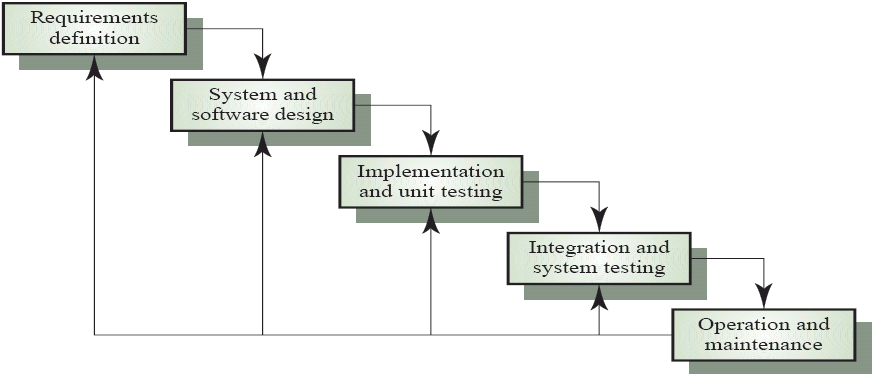
\includegraphics[height=150px,width=300px]{img/Waterfall_with_feedback.png}}
\caption{Waterfall with feedback} \cite{waterfall:feedback}
\label{fig:WaterfallFeedback}
\end{center}
\end{figure}

Even with the addition of feedbacks, the team felt that the waterfall model did not fit the rapid development, and possible changes in scope and requirements, of the project. 

\section{Requirements}
We are using a Scrum-like project management framework, and working \glspl{prototype} are expected to be produced at the end of every other sprint. Requirements have been prioritized by the customer on a scale from 1 to 100. Some of the requirements for our project are inevitably overlapping, and a significant part of the requirements must be accomplished in order to produce a working solution. This is reflected in the prioritization made by the customer. The requirements of the project are discussed in detail in chapter \ref{chap:Requirements}.

\section{Project plan}
This section describes the specific layout of the project. This project follows the Scrum methodology with some variants introduced, as discussed in section \ref{subsec:scrumadaptations}. The first five weeks were spent planning, pre-studying (which included a preliminary implementation of the critical part of the system), and writing the requirement specification. After this, the project was divided into sprints. We decided to make each sprint one week. At the end of the last sprint all the requirements should be accomplished.

\subsection{Phases}
After the initial phase of the project, and the production of the pre study, a total of 6 scrum sprints are planned:
\begin{itemize}
\item Initiation phase (pre-planning)
\item Project Planning
\item \Gls{pre-study} Sprint (Sprint 0)

\item Sprint 1
\item \Gls{pre-delivery} of report (17th October)

\item Sprint 2
\item Sprint 3
\item Sprint 4
\item Sprint 5
\item Sprint 6

\item Finish report
\item Prepare for presentation
\item Final Delivery and demonstration
\end{itemize}

In figure \ref{fig:gantt} the Gantt diagram for our project is presented:
\begin{figure}[h]
\begin{center}
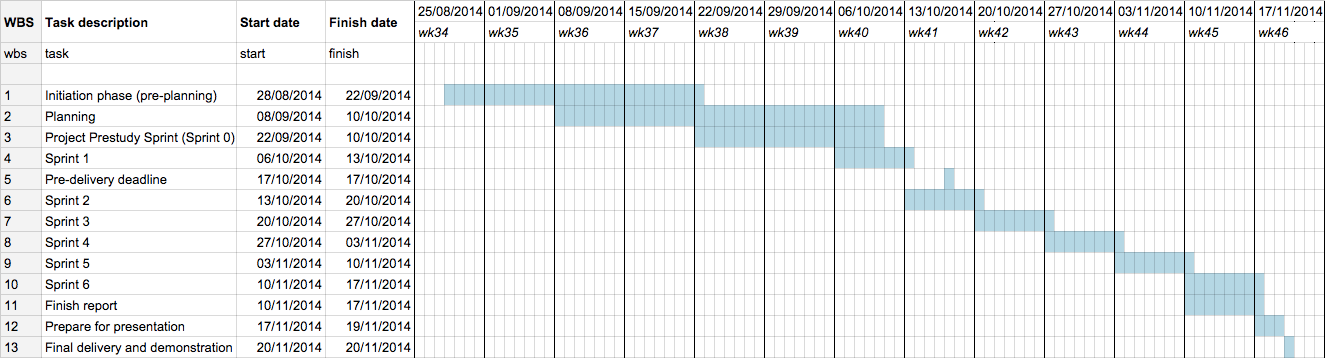
\includegraphics[height=130px,width=440px]{img/gantt.png}
\caption{Gantt diagram}
\label{fig:gantt}
\medskip
\small
\end{center}
\end{figure}

\subsection{Activities}
\begin{description}
\item[Pre-planning] During the pre-planning activity, the group members get to know each other and understand the task. There are also the first meetings with the customer and with the advisor.
\item[\Gls{pre-study} and planning] The \gls{pre-study} and planning activity is the stage where the actual work on the project begins. The group explores solutions, determine which technologies will be used, and how the product will be realized.
\item[Documentation] The documentation activity represents time spent documenting the work effort, including implementation, research etc., and administrative tasks like status reports and documents for the meetings.
\item[Coordination] The coordination activity is accomplished throughout the project, and consists of activities to coordinate the work, such as meetings, internal emails, calls and messages.
\item[Implementation] The implementation activity consists of the implementation of the system. This includes the programming of both the back end and the front end part.
\item[Testing] The testing activity represents time spent testing the system. This includes integration testing, unit testing, functional testing and scenario-driven testing.
\item[Presentation] The presentation activity is the final presentation of the system and the delivery of the report.
\end{description}

\subsection{Milestones}
To mark progress in the project, as well as making sure the team is clear on important deadlines, a set of milestones was set. Some of these are predefined in the course, and some are set by the group. 

The following milestones have been defined:
\begin{description}
\item[October 6th] \Gls{pre-study} phase to be completed
\item[October 17th] \Gls{pre-delivery} of report (defined by the course coordinators)
\item[November 17th] Project report to be completed
\item[November 20th] Final presentation day (defined by the course coordinators)
\end{description}

\subsection{Lectures}
In this projects there have been a number of guest lectures, and we have made sure that every lecture was attended by at least one member in the team.
The "Group Dynamics" lecture was mandatory, and everyone in the group attended it.
The other lectures that have been attended are:
\begin{itemize}
\item "How to sell in large application projects", Thomas B. Pettersen - Computas (01.09.2014)
\item "Scrum, agile development method", Torgeir Dingsoyr - SINTEF (02.09.2014)
\item "Estimation, agile/practical project work", Fredrik Bach - BEKK, (02.09.2014)
\item "Project management", Stian Mikelsen - Bearingpoint (15.09.2014)
\item "Technical Writing in English", Stewart Clark - \gls{NTNU} (24.09.2014)
\item "Sales techniques with exercises in groups", Morten Selven - Mikos (01.10.2014)
\end{itemize}

\section{Project Organization}
\subsection{Organizational diagram of how the group is organized}
In figure \ref{fig:organizational-structure}, the structure of the group is shown. 

\begin{figure}[h]
\begin{center}
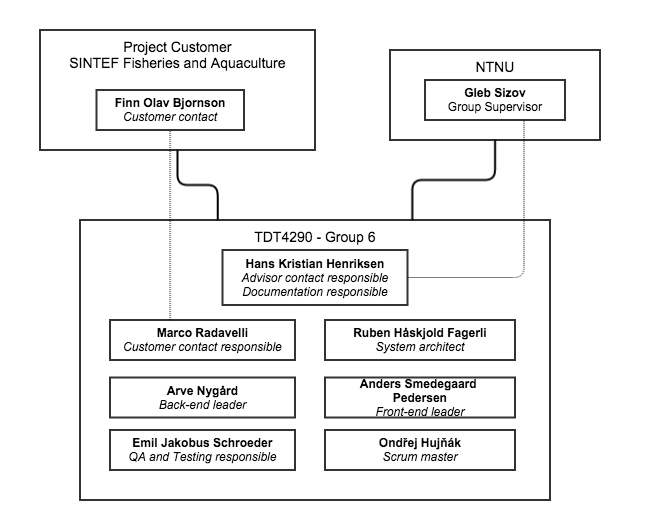
\includegraphics[height=260px,width=328px]{img/tdt4290_group_6_organizational_structure.png}
\caption{Organizational diagram.}
\label{fig:organizational-structure}
\medskip
\small
The arrows indicate bi-directional communication. The dotted arrows denotes the preferred way of communication between components. Note that the layout is not hierarchical and it is arranged this way only to better fit on the printed page.
\end{center}
\end{figure}

\subsection{Roles and corresponding responsibilities}
To have a clear division of responsibilities, the group chose to assign central roles early in the project. This was agreed upon through a combination of the wishes of each group member, and their technical insights and personal qualities. 

The group decided on the following roles,and their definitions:
\begin{description}
\item[Scrum master] The scrum masters task is to make sure that the group meets it's goals, he\footnote{"He" should be read as "he or she" throughout this report} is the leader of meetings, makes sure that the groups meetings have a structure, and that they finish on time. It is also the scrum masters task to make sure that the team meets deadlines, and finishes tasks. 

The scrum master is in standard scrum methodology tasked with being a barrier between the team and the surrounding environment. He should make sure that any distractions and uncertainties are taken care of, and let the rest of the development team focus purely on their tasks. In our project, this part of the scrum masters role has been difficult to implement, as the course requires all students to take part in activities that usually would be the scrum masters responsibility. 
\emph{Role assigned to: \textbf{Ondrej Hujnak}}

\item[Customer contact] The customer contacts responsibility is to arrange customer meeting, forward customer emails to the group if needed, and ensure that all the needed communication with the customer is done. As far as possible, no other members of the team should contact the customer directly. This will ensure that there is no double communication, as well as giving the customer a single contact in the team.
\emph{Role assigned to: \textbf{Marco Radavelli}}

\item[\gls{QA} and testing responsible] Ensures that the implementation fulfills the requirements, designs the test plan, defines and ensures that the Quality Assurance standard is followed during the project. Is responsible for making sure that sufficient testing is conducted.
\emph{Role assigned to: \textbf{Emil Jakobus Schroeder}}

\item[Documentation responsible] Supervises the structure and the content of all the documents the group produces during the project. This includes the \gls{pre-study}, \gls{pre-delivery} and final report. Is also the person responsible for taking minutes during meetings, and making sure that they reflect accurately what was said during the meetings.
\emph{Role assigned to: \textbf{Hans Kristian Henriksen}}

\item[Advisor contact] Arranges the advisor meetings, makes sure that all required documents are sent to the advisor before each meeting. Will, as far as possible, be the only person from the group communicating directly with the advisor on group specific matters.
\emph{Role assigned to: \textbf{Hans Kristian Henriksen}}

\item[\Gls{front-end} leader] The \gls{front-end} leader supervises the \gls{front-end} architecture and implementation, and coordinates the \gls{front-end} developer team. He is expected to have an overview of the process and plan ahead in the case of problems or blocked tasks.
\emph{Role assigned to: \textbf{Anders Smedegaard Pedersen}}

\item[\Gls{back-end} leader] Has the same role as the \gls{front-end} leader, but focuses on the back end team.
\emph{Role assigned to: \textbf{Arve Nygård}}

\item[System architect] The system architect makes sure that there is consistency between requirements, design and implementation, and that the design is feasible and reasonable.
\emph{Role assigned to: \textbf{Ruben Håskjold Fagerli}}
\end{description}

\subsection{Weekly schedule}
We decided to adopt a scrum-like model of software development, with internal group meetings twice a week, weekly meetings with the advisor and meeting with the customer when needed (typically every other week). The schedule is defined as follows:
\begin{itemize}
\item Mondays 2-3 pm - Advisor meeting
\item Mondays 3-4pm - Team meeting
\item Thursdays 12-2pm - Team meeting
\end{itemize}
For weeks 37 and 38 the advisor meeting will be Thursday 4pm.

\section{Risk assessment}
For a project this size and duration, there are a multitude of risks that needs to be taken into consideration. The team has identified the risks they feel are most relevant for the project, and attempted to classify them. The risks have two classes, probability and consequence. \textit{Probability} is the likelihood of the risk taking effect, while \textit{consequence} is the severity of the risk if it takes effect. We have assigned each risk class one of three ratings, \gls{L}, \gls{M} and \gls{H}. For each risk, a strategy has been developed to lower both the probability and consequence. 

An overview of risks and strategies is given in the following table:

  \begin{longtable}{p{0.7cm} p{2.5cm} p{0.7cm} p{0.7cm} p{6.5cm} }
  \caption[]{Risk assessment}\\
  \multicolumn{1}{p{0.7cm}}{ID} &
  \multicolumn{1}{p{2.5cm}}{Problem desc.} &
  \multicolumn{1}{p{0.7cm}}{Prob.} &
  \multicolumn{1}{p{0.7cm}}{Sev.} &
  \multicolumn{1}{p{6.5cm}}{Action}
  \endhead

  \caption[Risk assessment]{} \label{riskAss} \\
  \hline
  \multicolumn{1}{p{0.7cm}}{ID} &
  \multicolumn{1}{p{2.4cm}}{Problem description} &
  % \multicolumn{1}{p{0.8cm}}{\parbox[t]{0.8cm}{Proba-bility}} &
  % \multicolumn{1}{p{0.8cm}}{\parbox[t]{0.8cm}{Cons-equens}} &
  \multicolumn{1}{p{0.7cm}}{Prob.} &
  \multicolumn{1}{p{0.7cm}}{Sev.} &
  \multicolumn{1}{p{6.5cm}}{Action}
  \endfirsthead
  
  \hline
  \multicolumn{5}{r}{{Continued on next page}} \\
  \endfoot

  \hline \hline
  \caption[Risk assessment]{Here "Prob." stands for "Probability" and "Sev." stands for "Severity"}
  \endlastfoot

  \hline
%\begin{tabularx}{\linewidth}{lXllX}
R1 & Personal Conflicts & \gls{M} & \gls{M} & Might affect the quality of the work, motivation and time required. Probability can be reduced by ensuring communication within the group, and democratic and motivated decisions. \\ \\ \hline
R2 & Assignments given in other courses & \gls{H} & \gls{M} & Time for some students could be less than planned during a few weeks, due to intensive-demanding assignments of other courses. Mitigated by planning, frequent workload balancing and contributing with extra work in weeks without as intensive demands. \\ \\ \hline
R3 & Conflicting schedules & \gls{H} & \gls{M} & Reduced by planning meeting-times and communication channels for times between group meeting. Also, accepting that we can't meet every day and that all group members do not always need to be present. \\ \\ \hline
R4 & Solution is overcomplicated & \gls{M} & \gls{M} & Probability reduced by good communication both with the customer and internally in the group. \\ \\ \hline
R5 & Technical problems and difficulties & \gls{M} & \gls{H} & To reduce the probability: make a detailed study (and \glspl{prototype} where possible) during the \gls{pre-study} phase. To reduce the consequence: find the person/people within the group which are more comfortable with those new technologies and assign them that task if it is a particular task. Knowledge transfer within the team is also a way to reduce the consequences of this risk. Keep the customer informed. \\ \\ \hline
R6 & Missing room reservations & \gls{H} & \gls{L} & Will delay work. Avoid by making sure we have a regular room (talk to advisor) \\ \\ \hline
R7 & Data loss & \gls{L} & \gls{H} & Limited by introducing a backup strategy, and making sure that all team members follow this strategy. \\ \\ \hline
R8 & Assigned tasks are not completed & \gls{H} & \gls{M} & Consequence reduced by additional work for other group members in order to try to complete the task within the deadline. Talk within the group to find a compromise. Continuous communication between team members will help identify this risk early.  \\ \\ \hline
R9 & Illness & \gls{H} & \gls{M} & Probability cannot be reduced, but consequence can be reduced by temporary increase the work for other members of the group. One person should not be assigned tasks in a way that makes other team members unable to cover for them. \\ \\ \hline
R10 & Team members are late, or do not show, to meetings & \gls{H} & \gls{M} & Probability reduced by defining clear rules and schedules for the meetings. \\ \\ \hline
R11 & Team members cannot find meeting room for the meeting or misstake date and time & \gls{H} & \gls{M} & Probability reduced by creating a calendar shared by the group members and constantly updated. Ensure communication within the team. Reserve the same room and keep the same schedule for meetings. \\ \\ \hline
R12 & Cannot complete the product backlog or sprint backlog & \gls{M} & \gls{H} & Reduced by making sure to follow the priority of the tasks. The scrum master has a special responsibility to identify this situation early. \\ \\ \hline
R13 & Mistakes in the documentation or in the final product & \gls{M} & \gls{M} & Probability reduced by ensuring that every deliverable is reviewed and checked by at least one different person than the one who wrote it. Make sure to dedicate resources for software testing and review of documents. \\ \\ \hline
R14 & Malfunction of personal computer equipment & \gls{L} & \gls{M} & Probability cannot be reduced. Consequence can be reduced by increase work for other team members, and assign team members with malfunctioning equipment tasks that do not require a specific tool to be installed, so that university computers can be used for the work. \\ \\ \hline
%\end{tabularx}
\end{longtable}

\chapter{Tools and technology}
\label{chap:ToolsAndTech}
\section{Documents}

  \subsection{\LaTeX}
  \LaTeX~is a typesetting system and document markup language that became standard for scientific documents. It is easily expandable by thousands of different packages and can handle all aspects of scientific papers.

  We have chosen to use \LaTeX~for our report for two main reasons - \LaTeX~sources are easily readible and, because they are simple text files, they can be easily versioned by various version control systems. The second reason is focus on content, not on form. In \LaTeX~sources there is very little information about the exact view of the page. \LaTeX~itself during compile time chooses the best position of elements so it complies with all typographic norms.

  We have created a template in our shared space together with a bibliography file. All team members are then able to write his sections in an environment that suits him the best, while the current state of the report is always available to all members.

  \subsection{Google Docs}
  Google Docs \footnote{\url{https://docs.google.com}} is a web based office suite including a text editor, a spreadsheet program and a presentation program. All files created in these programs can easily be shared with colaborators. By sharing files, the colaborators get access to view and edit the files. It is also possible to edit and comment on other's work. We decided to use Google Docs for all documents that did not require the advanced typesetting of \LaTeX~so we had a common platform for such documents. This saves time, while still keeping documents backed up and accessible. 

\section{Project management}
  \subsection{Trello}
  \label{subsec:Trello}
  Trello \footnote{\url{http://www.trello.com}}is a web-based collaborative project management tool originally made by Fog Creek Software (New York, USA) \footnote{\url{http://www.fogcreek.com/}}. 
It's based on the Kanban method which has first implemented by Toyota in 1953 to be used in car production. It has since been modified to be used in several different industries. 
David J. Anderson formulated a model based on Kanban for knowledge based work, specifically software development, where the team incrementally pulls work from a queue \cite{da2004}. 
We use Trello for organizing our tasks into four states: "To do", "Doing", "Blocked" and "Done". The default state is "To do", and by changing the state of a task everybody in the group knows what needs to be done, what is being worked on, what tasks are dependent on other tasks or factors, and what tasks are done.
This is a simple yet efficient way of managing tasks. We chose Trello for the ease of use and the fact that it takes very little time to learn to use. In comparison, a system like Jira \footnote{\url{http://https://www.atlassian.com/software/jira}} has more features that might have been useful, but it takes more time and effort to learn. Therefor we have opted for Trello.
Trello is a freemium web service which means that it is free to use but additional support and features can be accessed if you pay a fee. As we only needed the standard functions we used the free version.
  \subsection{Slack}
  \label{subsec:Slack}
Slack is a web based team communication tool founded by Stewart Butterfield. It offers text chat in different channels and integration with a number of different popular services used by development teams \footnote{\url{https://slack.com/integrations}}. This has been useful to us since we needed to share information that might be more relevant to specific team members and also to have a single means of communication. Using Slack's integration with Trello and Github the team has been notified when there where changes on these platforms as well. Slack's capability to share files, or link to files on Google Documents, also came in handy.

\section{Version control}
  \subsection{Git}
  Git is a distributed version control system developed in 2005 by Linus Torvalds and Linux development community \cite{ProGit}. Git was made to be small, fast and easy to use especially for code management, as it's main purpose was versioning of Linux kernel source code. Nowadays, Git is one of the most used versioning controls systems in software development, thanks to it's open license and powerful features.

  We have chosen Git because some members already know it and are able to work efficiently with it. Another advantage is easy branching and distributed architecture that allows you to work offline. 
  
  We have created an organization on GitHub\footnote{\url{https://github.com}} with multiple repositories for different separate parts of our work - reports, server sources, client sources. We have chosen GitHub because it is well known, and because of the git hosting server that offers advanced features and stability. Moreover, some members already had accounts on GitHub and were familiar with the interface, which shortened time needed to setup a working environment.

\section{Programming languages}
The choice of implementation language, platform and tools to use is left up to the group. The customers only requirement is that the solution should be able to run in their environment.
  \subsection{Java}
  Java is a popular programming language developed by a team led by James Gosling at Sun Microsystems in 1991. It's full-featured, general purpose, language capable of developing robust mission-critical applications \cite{liang}. This and the fact that everybody in the group had at least basic knowledge of Java led to the decision that we would use Java for our \gls{back-end} application.  
  \subsection{JavaScript}
  As stated by Davis Flanagan in "JavaScript: the definitive guide": 
  \begin{quote}
  "Javascript is part of the triad of technologies that all Web developers must learn".
  \end{quote} 
  He continues to note that JavaScript specifies the behavior of the web page \cite{fd11}. Along with specification of \gls{HTML5} and ECMAscript 6 (the standard name of JavaScript) the possibilities of what you can achieve with JavaScript has greatly improved. Since our assignment is to create a web based solution, it seams natural to use JavaScript as part of the solution. This is further supported by the existence of \gls{open source} libraries designed to make interactive maps, which is relevant for our assignment.

\chapter{Pre study}
In this chapter, we present the findings of the pre study. The pre study document was made as a separate document that was meant to be delivered to the customer independently of this report. Therefore, there are overlapping sections with the full report. These sections will not be given in this chapter, but are instead presented in their respective chapters of the full report. 

\section{Background}
To get an understanding of the customers needs, as well as studying different solutions, a pre study is conducted. From the \gls{course compendium}:
\begin{quote}
The preliminary studies are vital for the group to obtain a good understanding of the total problem.
Here, you will have to describe the problem at hand. You should describe the current system and the
planned solutions (...).
\cite{TDT4290:Intro}
\end{quote}

\section{Current situation at SINTEF}
In this chapter we will explore the solution SINTEF is currently using, and the challenges and limitations it poses. After looking into this, we will describe the evaluation criteria that will be used to assess the alternative solutions the group has found. 
\subsection{Current system}
\begin{figure}[h]
\begin{center}
\fbox{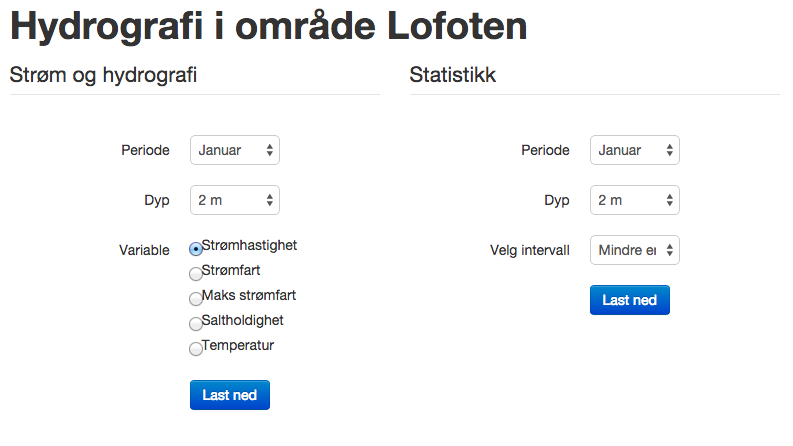
\includegraphics[height=223px,width=396px]{img/region_interface_sinmod.png}}
\caption{The main interface for a region in SinMod}
\label{fig:sinmod-region-main-interface}
\end{center}
\end{figure}

The current system deployed at SINTEF serves their clients by providing access to a collection of more than 100 000 pre generated PDF files. These files contain information on currents, salinity, and temperature. The user may choose what information he wants by selecting parameters in the drop down menus, see figure \ref{fig:sinmod-region-main-interface}.

\begin{figure}[h]
\begin{center}
\fbox{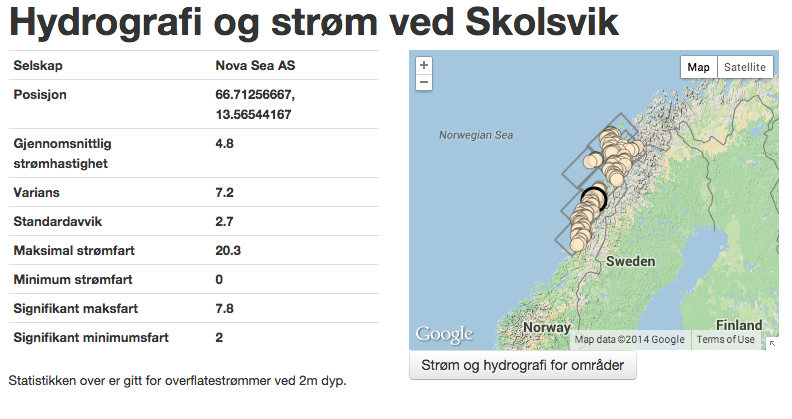
\includegraphics[height=223px,width=396px]{img/site_key_data.png}}
\caption{The key data a user is presented with when selecting a specific site}
\label{fig:sinmod-site-key-data}
\end{center}
\end{figure}

If the user chooses a specific site from the map or location drop down, he will be presented with key data for this area. This includes statistical information such as maximum current speed, average current speed and so forth, as well as geographical position, as given in figure \ref{fig:sinmod-site-key-data}.


\begin{figure}[h]
\begin{center}
\fbox{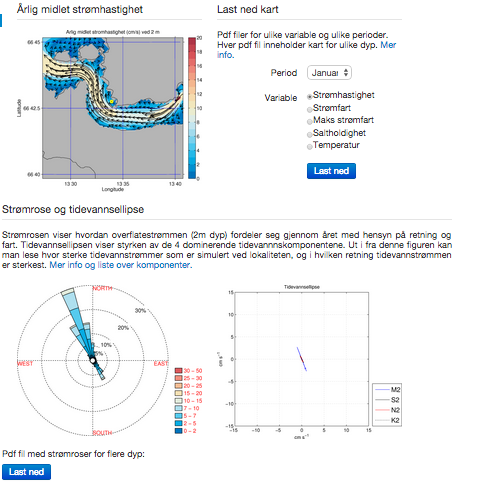
\includegraphics[height=300px,width=300px]{img/site_graphs.png}}
\caption{Some of the graphs presented to the user when selecting a specific site}
\label{fig:sinmod-site-graphs}
\end{center}
\end{figure}

The system will also present a set of pre defined graphs, including current roses, tidal ellipsis and vertical profiles. The graphs are given for standard attributes (e.g depth 2 meters), and for some of them, there is an option of downloading a PDF containing graphs for other values of the given attributes. An example is shown in figure \ref{fig:sinmod-site-graphs}


\subsection{Challenges}
As the PDFs are pre generated, there is a clear limitation to what information the user may request. If a user wants to know, for example, the connection between salinity and current speed at a given location, the user must download two different PDFs and manually compare these. 

The graphs given for a specific location are only given for limited values of the critical attributes. If we look at the current rose, it is presented for a depth of 2 meters. If the user is really interested in the current rose for 10 meters, he has to download the PDF containing all possible current roses. 

The same is true for the maps that can be generated for a specific site. The user may choose period (a single month may be selected), and one of the five variables. This gives the user a PDF with one map for each depth that can be calculated. 

For a user who knows what data is interesting, this is a complicated and data heavy way of delivering information. The PDFs seems to range in size from 125kB to around 3MB, depending on what information is requested. The region maps are the absolute largest in file size, ranging from 1 to 3MB, while the files containing the current roses are quite small, in the 100-200kB range. 

On a computer with broadband connection, the size of the files is not very problematic. For these users, the biggest challenge is the fact that the user can not specify what kind of data they want plotted, and have to look through quite a lot of pages to get the information needed. For a user on a low bandwidth connection and/or on a mobile device, the size of the files is a more pressing problem. On an \gls{EDGE} connection the theoretical best download time for a 3MB file is 62,5 seconds at 384kbit/s \cite{3gpp.com}.

\subsection{Evaluation criteria}
SINTEFs main goal with this project is to be able to rid themselves of the PDF store, and generate the information on demand. This will make for a much more flexible system, where it will be possible to add new graphs and functionality quickly. For the customers, it will make it possible to request more customised graphs and plots.

SINTEF has presented the group with several goals they wish the new system to fulfill:

\begin{itemize}
\item The system should generate the graphs and maps directly from the \gls{netcdf} files on user request.
\item The user should be able to select several variables for one plot.
\item The system should be usable on low bandwidth connections.
\item The system should be usable on mobile devices.
\item The system should be easy to expand with new functionality.
\end{itemize} 

With these goals in mind, the group started looking into different technologies that could be used to make such a system.

%%%
\section{Other production solutions}
The group has used the first part of the project investigating what solutions would best suit SINTEFs needs. In the chapter we present the different solutions we have found, along with an assessment on how each solution is rated in accordance to the evaluation criteria. 

%Existing tech - Italian solution
\subsection{Adriatic Forecasting System}
\emph{Link: \url{http://oceanlab.cmcc.it/afs/}} \\%make sure to use //
  The solution, by the Operational Oceanography Group Italy and cmcc Ocean-Lab, can display temperature, salinity, currents, sea surface height, wind stress and heat flux. It allows the user to choose date, region and depth as search filters, and uses \gls{PNG} overlays on a Google map. The PNGs are retrieved from cmcc's own server.
  Although it graphically looks quite nice, it can be seen that some tiles are not precisely overlapping. In addition, sometimes it is needed to refresh the page because the application doesn't load properly. \gls{PNG} layers are displayed without a specific JS library, and the JS code is quite complex compared to other existing solutions using libraries. Therefore this solution is not well re-usable.
\\ \emph{Overall rating: \textbf{Ok}}

\subsection{Danish Centre of Ocean and Ice}
  \emph{Link: \url{http://ocean.dmi.dk/anim/index.uk.php }} \\%make sure to use //
    The solution by the Danish Center of Ocean and Ice can display temperature, salinity and current, which are the most important factors of the SINTEF simulation. This said, it lacks the ability to choose depth and specify a date interval. The data is shown as static PNGs, thus the map is not interactive. There is, on the other hand, a possibility to choose different geographical areas with the highest level of detail around Denmark. This is on the same level as SINTEF's existing solution.
  \\ \emph{Overall rating: \textbf{Bad}}

  \subsection{Fisheries and Oceans Canada}
  \emph{Link: \url{http://www.tides.gc.ca/eng}} \\%make sure to use //
    The solution of the Canadian government resembles the Danish one. It is possible to choose a geographical area on a static map. By choosing an area you get the opportunity to choose a smaller, more specific area. The big difference is that all data is presented as text in tables, thus making it less convenient and intuitive to use.
  \\ \emph{Overall rating: \textbf{Bad}}

  \subsection{Ocean viewer}
  \emph{Link: \url{http://www.oceanviewer.org}} \\%make sure to use /
    Ocean Viewer is a pilot project of the \gls{MEOPAR} of Canada. It gathers data from different sources and displays it as PNGs overlayed on a map. You can select different geographical areas on a customized Google Map and different data from a menu (temperature, salinity and others). Like the Danish solution the PNGs can be shown in sequence to show changes over time.
  \\ \emph{Overall rating: \textbf{Ok}}

  \subsection{Sea temperatures and Currents - Bureau of Meteorology}
  \emph{Link: \url{http://www.bom.gov.au/oceanography/forecasts/}} \\%make sure to use //
    The Australian Bureau of Meteorology has a solution that is very similar to the other national agencies. You can choose a geographical area on a static map. Here as well, the data is visualized with images overlayed on a static map, with the possibility to loop through the images to show changes in the data over time.
  \\ \emph{Overall rating: \textbf{Ok}}
  
  \subsection{yr.no Map Service}
  \emph{Link: \url{http://yr.no/kart}} \\%make sure to use //
This solution presents the user with a conventional map interface. On the sides and top there are menus for selecting which variable and timestep should be displayed. The user is only allowed to select a timestep about 8 days from the current time. Interesting variables include sea temperature, salinity and sea currents, each has it's own . There is no way to select depth, and all data seems to be for the surface values. The chosen variable is added as an overlay of \gls{PNG} tiles using OpenLayers. The tiles are fetched using \gls{WMS} from a norwegian meteorological service server. On the map there are several measurement stations displayed, that give information when clicked. In addition, clicking anywhere on the map displays several plots predicting the next two days of weather for that spot.
  \\ \emph{Overall rating: \textbf{Ok}}

\section{Back-end}

\subsection{GeoServer}
Does not support \gls{netcdf} natively. There exist a community plugin that enables you to read from \gls{netcdf} files, but the support seems very shifty. GeoServer does not seem to have support for more than one file and metadata appears difficult to extract. Due to this factors, the system was deemed to not to meet the needed criteria.

\subsection{THREDDS}
\begin{quote}
The \gls{THREDDS} Data Server (TDS) is a web server that provides metadata and data access for scientific datasets, using \gls{OPENDAP}, \gls{OGC} \gls{WMS} and \gls{WCS}, \gls{HTTP}, and other remote data access \glspl{protocol}. \cite{TDS:Web}
\end{quote}

  Except supporting multiple data access \glspl{protocol}, \gls{TDS} is able to virtually aggregate multiple \gls{netcdf} files to one dataset that can be used for queries, such as selecting a region and sending it's data in specified format. Dataset configurations are done via \gls{NCML}, which is a dialect of \gls{XML}.

  Although \gls{TDS} seems to support everything that is needed for this project, it's installation, and especially configuration for agreggation and special needs, is not trivial. Moreover there are doubts about speed and dealing with serving a range containing large quantified points. One advantage is that SINTEF currently have a \gls{TDS} running and configured, so we won't need to configure it from scratch, and SINTEF employees probably have experience and knowledge about setting it up, something which the group lacks.

  \subsection{Custom solution}
  An alternative is to write a custom \gls{back-end} from scratch.
  Advantages of this are:
  \begin{itemize}
  \item Easy deployment - written as a single service that you just launch.
  \item Load balancing - Easily scale outwards: The servers can be put behind a load balancer. 
  \item Speed - No overhead for unused features.
  \item Code clarity - No overhead for unused features.
  \end{itemize}
  A skeleton for the whole server is in place. Below is a list of features that the group feels are within reach in the project period. 
  \begin{itemize}
  \item Indexing and file selection.
  \item Projection (Mapping between latitude/longitude and file indices)
  \item Filtering (Reducing the result set before reading the file)
  \item Output
  \item Rendering to image
  \item Rendering to GeoJSON
  \end{itemize}

  Performance seems to be very good at the current level of implementation. The only major potential bottleneck the group sees is reading files from a hard-drive. (All testing has been done on \gls{SSD}). This bottleneck will however be independent of \gls{back-end} solution.
  
  \subsection{MapTiler}
  \emph{Link: \url{http://www.maptiler.org/}} \\%make sure to use //
    MapTiler is an application for online map publishing. It makes it possible to create tiles that can be overlayed over other maps like Google Maps, Open Street Map and others. It's written in C/C++ and claims to be a lot faster than other existing solutions. A draw back seems to be that it's made for overlaying a pre generated directory of images rather than dynamic data like the ocean forecast data.
  \\ \emph{Overall rating: \textbf{Ok}}
  
    \subsection{ncWMS}
  \emph{Link: \url{http://www.resc.rdg.ac.uk/trac/ncWMS/}} \\%make sure to use //
    ncWMS is an \gls{open source}, free to use, java server application. It was created to support interactive browsing of gridded four-dimensional \gls{netcdf} data over the web. Clients will send request containing the wanted coordinates (latitudes, longitudes, depth and time), what variable is to be displayed, projection, format and size the response should be. ncWMS, which has been configured to read from datasets (for example sets of \gls{netcdf} files or a \gls{THREDDS} server), responds to a request with an image of the desired type. ncWMS adheres to the \gls{WMS} specification (\gls{WMS} 1.3.0 and 1.1.1 are supported).
    \paragraph{Configuration}
    ncWMS is mainly configured through a web interface, where you can add datasets and change server settings. A dataset can be: a single \gls{netcdf} file, an \gls{OPENDAP} endpoint (a service provided by \gls{THREDDS}), a NcML file or a glob aggregation (using wildcard characters like ). It is possible to configure which variables of a dataset to expose and how. Each dataset can also be set to automatically refresh at certain intervals. The server can be set to cache data, to reduce \gls{CPU} load at the expense of memory and disk space.
    \paragraph{Aggregation}
    The glob aggregation or NcML work well with files that cover the same area, but contain different timesteps. To handle different areas and different resolutions it may be possible to use \gls{THREDDS}/\gls{OPENDAP} or NcML.
    \paragraph{Perfomance}
    Testing both local and publicly available ncWMS servers the performance seems good. When using the godiva2 browser based client or sending individual requests the server mostly responds quickly, with some idiopathic exceptions. Transmitting the map data to the client as \gls{PNG} images should be a bandwidth-efficient way to do it, as well as moving the computation load away from the client. When starting the server application or adding a dataset, the server needs some time to load some information from the datasets. This only takes a few seconds, even for a few hundred GB of local \gls{netcdf} files.
    \paragraph{Summary}
    ncWMS does a lot of what we need the \gls{back-end} of our solution to do. It handles the extraction, downsampling and projection of the data, creating an image ready to be used in a map widget or on it's own. It can only handle requests for a few kinds of plots. It is \gls{open source}, and is free to use under a modified \gls{BSD} license. To serve all the plots and data required it would need modification.
  \\ \emph{Overall rating: \textbf{Good}}

%%%
\section{Transmission Protocols}
  There are several standardized \glspl{protocol} to present map data from the server to the client in order to dynamically display layers on a map.
  In particular, two main kind of representations can be distinguished, and sometimes they're both supported by a single standard:
  \begin{description}
    \item[Vector based layers] Data is sent from the server to the client in a textual format, such as GeoJson
    \item[Image based layers] Data is sent from the server to the client as images, such as \gls{JPEG}, \gls{PNG} and \gls{GIF}
  \end{description}

  The \acrfull{OGC} became involved in developing standards for web mapping after a paper was published in 1997 by Allan Doyle, outlining a "WWW Mapping Framework". The oldest and most popular standard for web mapping is \gls{WMS}. However, the properties of this standard proved to be difficult to implement for situations where short response times were important. For most \gls{WMS} services it is not uncommon to require 1 or more \gls{CPU} seconds to produce a response. For massive parallel use cases, such a \gls{CPU}-intensive service is not practical. To overcome the \gls{CPU} intensive on-the-fly rendering problem, application developers started using pre-rendered map tiles. Several open and proprietary schemes were invented to organize and address these map tiles. 
  In order to reduce the performace problems of \gls{WMS}, new standards have been defined:
  \begin{itemize}
    \item TMS
    \item WMS-c
    \item WMTS
  \end{itemize}
  
  \subsection{WMS}
    \acrfull{WMS} is a standard \gls{protocol} for serving georeferenced map images over the Internet that are generated by a map server using data from a GIS database. The specification was developed and first published by the Open Geospatial Consortium in 1999.
    A \gls{WMS} server usually serves the map in a bitmap format, e.g. \gls{PNG}, \gls{GIF} or \gls{JPEG}. In addition, vector graphics can be included: such as points, lines, curves and text, expressed in SVG or WebCGM format.
    The \gls{WMS} standard allows flexibility in the client request enabling clients to obtain exactly the final image they want. A \gls{WMS} client can request that the server creates a map by overlaying an arbitrary number of the map layers offered by the server, over an arbitrary geographic bound, with an arbitrary background color at an arbitrary scale, in any supported coordinate reference system.

  \subsection{TMS}
\gls{TMS} is a specification for storing and retrieving cartographic data, developed by the Open Source Geospatial Foundation. The \gls{TMS} \gls{protocol} fills a gap between the very simple standard used by OpenStreetMap and the complexity of the \gls{WMS} standard, providing simple \gls{URL} to tiles while also supporting alternate spatial referencing system.
    \gls{TMS} is most widely supported by web mapping clients and servers, and it is served as the basis for \gls{WMTS} (the OpenGIS Web Map Tile Service \gls{OGC} standard).

  \subsection{WMS-c}
    The WMS Tiling Client Recommendation, or WMS-C for short, is a recommendation set forth by OSGeo for making tiled requests using \gls{WMS}. It is just a recommendation on using \gls{WMS} properly in order to improve performance by caching data.
    This recommendation relies on two basic concepts to support this purpose: First, cachability of map imagery can be improved by using image tiles of fixed width and height, referenced to some fixed geographic grid at fixed scales. A valid tile request is one that conforms to the specification of fixed image parameters and geographic grid(s) for a given layer. By analogy, an invalid tile request is one that does not.
    Second, caching of \gls{HTTP} GET requests is further made possible by constraining the \gls{URL} parameters used in the request. This recommendation identifies the \gls{WMS} GetMap parameters minimally needed for a client to request a valid tile.

  \subsection{WMTS}
\gls{WMTS} is a standard \gls{protocol} for serving pre-rendered georeferenced map tiles over the Internet. The specification was developed and first published by the Open Geospatial Consortium in 2010
    \gls{WMTS} builds on efforts to develop scalable, high performance services for web based distribution of cartographic maps. To define this standard, similar initiatives were also considered, such as Google maps and NASA OnEarth. \gls{WMTS} includes both resource (RESTful approach) and procedure oriented architectural styles (KVP and SOAP encoding) in an effort to harmonize this interface standard with the OSGeo specification.
    \gls{WMTS} complements earlier efforts to develop services for the web based distribution of cartographic maps. The \gls{OGC} \gls{WMTS} provides a complementary approach to the \gls{OGC} \gls{WMS} for tiling maps. \gls{WMS} focuses on rendering custom maps and is an ideal solution for dynamic data or custom styled maps. \gls{WMTS} trades the flexibility of custom map rendering for the scalability possible by serving of static data (base maps) where the bounding box and scales have been constrained to discrete tiles. The fixed set of tiles allows for the implementation of a \gls{WMTS} service using a web server that simply returns existing files. The fixed set of tiles also enables the use of standard network mechanisms for scalability such as distributed cache systems.

  \subsection{Summary}
    WMS-C is the best supported and most mature \gls{protocol}, but it's a bit of a kludge overlayed on top of \gls{WMS} to support tiles and it incurs some extra overhead from having to use world coordinate bounding boxes rather than tile coordinates.
    \gls{TMS} is fairly mature, and is specifically designed for tiles, but is not an official \gls{OGC} spec.
    \gls{WMTS} is an \gls{OGC} spec that is meant to replace \gls{TMS} and WMS-C. It works purely in tile coordinates like \gls{TMS} (although it computes them differently) but has some additional capabilities that weren't in \gls{TMS}, like GetFeatureInfo. It's comparatively recent, but it is becoming more and more used, even if its implementations are less mature. It is also supported by OpenLayers.

%%%
\section{Front-end solutions}
  A central part of the product requirement is to display simulated data in a dynamic manner. There exists solutions to do just that, and javascript libraries than makes it relatively easy to create at front end solution of our own. In this section we will discuss and compare the most relevant of these in the context of our assignment and the product requirements. 
  \subsection{Custom made solution}
    A custom made solution has the general advantage that we can built it to specification and thus make sure it meets the requirements without having to deal with other peoples code base. Trying to customize an existing solution might be as much work as building something from the bottom. In the following paragraphs we will review and rate technologies we found relevant for building a custom front end.
    \subsubsection{LeafletJS}
    \begin{tabular}{|p{4cm}|p{8cm}|}
      \hline
      Home page: & \url{http://www.leafletjs.com} \\
      \hline
      Service functionality: & Creating mobile-friendly interactive maps. \\
      \hline
    \end{tabular}
    
    \paragraph{Introduction} \indent
    LeafletJS ("Leaflet" for the rest of the section) is an \gls{open source} javascript library for creating mobile-friendly interactive maps. It's licensed under the \href{'https://github.com/Leaflet/Leaflet/blob/master/LICENSE'}{2-clause \gls{BSD} License}, which makes it free to use in commercial applications as long as a credit is added somewhere in the user interface.
    Even though Leaflet is free to use it is dependent on a third party to provide the map tiles. These may not be free to use.

    \paragraph{Features}
    Leaflet has the features you'd expect from a modern interactive map. This includes paning with inertia, zooming and the ability to add markers. It also supports double-tap and pinch to zoom for IOS and Android on mobile phones. Furthermore all the five biggest web browsers are supported, including graceful fallback for old versions.
    
    The most powerful feature of Leaflet is the ability to add layers. The different supported layers are:

    \begin{itemize}
      \item Tile layers
      \item Marker layers
      \item Pop-ups
      \item Vector layers
      \item GeoJSON layers
      \item Image overlays
      \item \gls{WMS} layers
      \item Layer groups
    \end{itemize}

    For our purposes the ability to get map tiles from different sources may be very interesting. This gives us the ability to for example show both nautical maps and regular land maps at the convenience of the user. At zoom levels covering large geographical areas it will probably be most ideal to show the relevant simulated data as overlayed PNGs. This is easily achieved with image overlays in Leaflet. If we want to show very detailed data when zoomed further in, we might be able to use vector layers to visualize the data. It is also possible to use a GeoJSON layer to convert data formatted as GeoJSON to vectors.
    It is also possible to use \gls{WMS} to overlay, for example, metrological data on a map. Eventhough this is a format that is used by large organizations like the National Oceanic and Atsmopheric Administration (\url{noaa.gov}) we have been advised against using this format due to it's negative effect on the speed and responsiveness experienced by the end-user. \footnote{Iván Sánchez Ortega, How to Build Slow Maps - Trondheim, September 24, 2014}
    Furthermore Leaflet can be extended with plugins. These can relatively easily be written in Javascript or an existing plugin can be downloaded and used. A relevant plugin to our needs could for example be heatmap.js (\url{http://www.patrick-wied.at/static/heatmapjs/}).

    \paragraph{Summary}
    Leaflet is very suitable for our needs in respect to creating an interactive map overlayed with visualizations of relevant data created by the SINTEF ocean forecast simulations. It's lightweight(33 kilobytes), made to be compatible with mobile phones and very flexible in possibilities to display data on maps. It's also well documented.

  \subsubsection{OpenLayers}
   \begin{tabular}{|p{4cm}|p{8cm}|}
     \hline
     Home page: & \url{http://openlayers.org/} \\
     \hline
     Service functionality: & A high-performance, feature-packed library for all your mapping needs. \\
     \hline
   \end{tabular}
   \paragraph{Introduction} \indent
   OpenLayers is an \gls{open source} (provided under the \href{'https://tldrlegal.com/license/bsd-2-clause-license-(freebsd)'}{2-clause \gls{BSD} License}) JavaScript library for displaying map data in web browsers. It provides an \gls{API} for building rich web-based geographic applications similar to Google Maps and Bing Maps. The library was originally based on the Prototype JavaScript Framework. Since November 2007 OpenLayers is an Open Source Geospatial Foundation project.
   The current stable version, OpenLayers 3.0, has been released August 29, 2014.
   \paragraph{Features}
   OpenLayers provides support to the following functionalities:
   \begin{description}
     \item[Tile layers] It pulls tiles from OSM, Bing, MapBox, Stamen, MapQuest, and any other XYZ source you can find. \gls{OGC} mapping services and untiled layers also supported.
     \item[Vector layers] Renders vector data from GeoJSON, TopoJSON, KML, GML, and a growing number of other formats.
     \item[Fast \& Mobile Ready] Mobile support is out of the box, and it is possible to build lightweight custom profiles with just the needed components.
     \item[Cutting Edge \& Easy to Customize] Map rendering leverages WebGL, Canvas 2D, and \gls{HTML5}. Map styling is controlled with straight-forward \gls{CSS}.
   \end{description}
   \paragraph{Initial load time}
   The initial load time of the map is ok on a PC. The total loading time of the example (\gls{HTML} with map and \gls{WMS} tiles) took around 4 seconds. The size of the Javascript library (ol.js) is 129 KB, and the first time (without any sort of browser caching) it was fetched in 473 ms.
   \\ \emph{Score: \textbf{Med}}
   \paragraph{Responsiveness}
   It's quite fast when pan, but not so fast when zooming in (438 ms + 2.43 s for DNS lookup of the \gls{WMS} server in the example) or out (around 400 ms was logged, on average, as the time to get tiles from the server, because there is no need of DNS lookup, but the overall perceived time is around 1s).
   \\ \emph{Score: \textbf{Med}}
   \paragraph{Detail and dynamism}
   The detail of the image is defined by \gls{PNG} provided by the \gls{WMS} server. Vector layers are also well drawn. Tile layers are updated on zooming.
   \\ \emph{Score: \textbf{High}}
   \paragraph{Ease of use}
   It is quite easy to implement. The code needed is low, and it is easily convertable into Leaflet format. There are a lot of provided working examples, but it is not well documented yet for the version 3.0 (that has been released very recently: at the end of August 2014). Anyway, the detailed \gls{API} documentation is provided.
   \\ \emph{Score: \textbf{Med}}
   \paragraph{Summary}
   It is a library used in a lot of applications, dynamic, with a lot of features. On the contrary, it is less lightweight than LeafletJS, not so well documented and not always so fast as experienced by the user, especially in zooming.
   \\ \emph{Overall rating: \textbf{Good}}
  
  \subsubsection{Wind map}
  \emph{Link: \url{http://hint.fm/wind/}} \\%make sure to use //
    Wind map is a personal art project that gets surface wind data from the American government agency National Digital Forecast Database and displays it as moving curved lines on a map. This makes for a very intuivive visualization of the data that give a good general picture of the actual real-world situation. It's zoomable and can pan. By clicking on a specific point on the map you get the wind speed and coordinates of the point. A draw back might be the use on moblie devices which may be suboptimal.
  \\ \emph{Overall rating: \textbf{Good}}

  \subsubsection{Comparison of Leaflet and OpenLayers}
    For the purpose of creating an interactive map we've boiled it down to either using LeafletJS or OpenLayers. As the description of each of the individual libraries above shows, the two are have many of the same capabilities. Both gives us the posibility to overlay visulizations of data in different ways. An reason for choosing Leaflet is the extensive documentation of the current version, a point where OpenLayers are lacking at the moment. Despite this OpenLayers support of \gls{WMTS} and \gls{WMSC} is such a strong argument in it's favor that we jugde it as the best fit for our purposes.
    
  \subsection{Godiva2}
     \begin{tabular}{|p{4cm}|p{8cm}|}
     \hline
     Example page: & \url{http://behemoth.nerc-essc.ac.uk/ncWMS/godiva2.html} \\
     \hline
     Service functionality: & A browser client made to browse data served by a ncWMS server. \\
     \hline
   \end{tabular}
   
  \paragraph{Introduction}
  Godiva2 was created as a companion for ncWMS, to display the pngs served by ncWMS as tiles in a map interface. It is a fairly simple \gls{HTML} page using JavaScript. \\
   It presents the user with a pannable, zoomable map interface of the earth. Variables (for example ocean temperature) can be selected from a menu. An overlay is added to the map, and the map zooms and pans to show the relevant area. The user can select the date, time of day and depth, updating the map immediately. Clicking on the map brings up a context menu, where a vertical profile plot can be created for that spot. Selecting a tool in the map interface, the user can draw a line on the map, and a plot is created showing the value of the selected variable along that line. There is a menu to select a different \gls{WMS}, changing the background map and projection of any overlays. The site allows the user to grab a permalink of the current state of the map.

	\paragraph{Load time}
	Before selecting a variable, only a list of available variables and the background map are fetched. Testing Godiva2 on a local ncWMS server the initial load time is low. Tests using publicly available datasets vary, but some have low load time, indicating that the slower ones might just have less available resources.
   \\ \emph{Score: \textbf{Good}}
	
	\paragraph{Responsiveness}
	The responsiveness of panning and zooming the map, as well as changing the desired depth and timestep varies quite a bit. This is true both for local and remote datasets.
   \\ \emph{Score: \textbf{Medium}}
	
	\paragraph{Detail and dynamism}
	Every bit of detail available in the dataset is shown, as required by the level of zoom.
   \\ \emph{Score: \textbf{High}}
	
	\paragraph{Ease of Use}
	The menus for changing variable, depth and timestep are all intuitive and easy to use. The map interface follows the conventions for zooming and panning with the mouse.
   \\ \emph{Score: \textbf{High}}
	
	\paragraph{Summary}
	This is a product made to browse 4 dimensional geospatial data like the ones we want to present. The look and feel is slightly outdated, but the functionality it has works well. It is \gls{open source}. It and the third party libraries are licensed under free software licenses. It (and the ncWMS server) would need to be modified in order to display all the data and charts found in the current solution.
   \\ \emph{Overall rating: \textbf{Good}}
	

\section{Recommendation}
Based on the study of possible solutions in the previous chapter, the group has made the following recommendation to the customer.

\subsection{Front-end}
As the group has looked into the situation at SINTEF, as well as other solutions in production, the conclusion is rather clear. SINTEF requires a very specific front end, with custom graphs, and the ability to add more functionality at a later stage. As far as existing solutions go, only the Godiva2 system has been close to performing the necessary tasks to serve SINTEFs needs. This system is however not very easy to adapt, and the group is of the opinion that changing this system to fit custom needs may be too much work to justify.

With this in mind, the group feels that the only realistic solution for the \gls{front-end} is to develop a custom system from scratch.

\subsection{Back-end}
For the \gls{back-end}, the group is divided in its recommendation. From our investigation into different technologies, it seems like \gls{THREDDS} is a solution that is generally implemented for working with \gls{netcdf} files. Advantages of using this is that there exists documentation, maintenance, and updates. The group has had trouble configuring \gls{THREDDS}, and has also gotten the impression that SINTEF is not perfectly satisfied with its performance. 

The group feels confident that a custom \gls{back-end} \gls{prototype} can be made, and that it will be able to meet the requirements. This will give the customer more flexibility in functionality and expandability, but will obviously not be as complete or well supported as \gls{THREDDS}.

The group asks SINTEF to make a decision for a \gls{back-end} solution based on the information in this report.

\subsection{Different paths}
As SINTEF is given a choice for how to proceed, the group sees two paths forward in the project:
\begin{enumerate}
\item \gls{THREDDS} \gls{back-end}: Given that SINTEF chooses to use a \gls{THREDDS} \gls{back-end}, the group asks SINTEF to provide a configured \gls{THREDDS} server. The group will focus their work on the \gls{front-end}, and attempt to make a \gls{prototype} that replicates most functionality from todays site.
\item Custom \gls{back-end}: Given that SINTEF chooses a custom \gls{back-end}, the team will split into two groups, and attempt to make a \gls{prototype} \gls{back-end}, as well as a \gls{prototype} \gls{front-end}. In this scenario, both the front- and \gls{back-end} will have limited capabilities, but will demonstrate what is possible with a fully custom solution.
\end{enumerate}


\chapter{Requirements}
\label{chap:Requirements}
This chapter presents the functional and non-functional requirements for the project, as well as system backlog priorities and estimates.

\section{Use Cases}
The desired behavior of the system can be described through use case diagrams. Here we will display the users and how they want to interact with the system. Use cases model the system requirements and is an easy way to understand which features are needed and how these features should work. This section will outline the general use cases. For more defined specifications we refer to the requirements specification in section \ref{reqspec}.

  \subsection{Planning}
  In our project, we have a relatively simple set of users and control of parameters. The main focus of our task is to deliver a full system with working \gls{front-end} and \gls{back-end} modules. In this case the user should be able to use the \gls{front-end} without further knowledge about the \gls{back-end}. The user will interact with a \gls{GUI} through key-input and mouse-input. This will mainly be map-interaction like scrolling or dragging the map, but parameters will also be controlled through buttons and other input fields.

  There is also a second type of users that is not as important in our scope, but will have to be considered. This is 3rd-party users or companies that request access the data directly from our \gls{back-end} for use with their own \gls{front-end} solution. These users will send requests over REST with commands from an \gls{API} for allowed requests.

  \subsection{Users}
  Our product will have two types of users:
  
  The \textbf{end-user} is a user that uses our \gls{front-end} solution, which again depends on our \gls{back-end} solution. Among such users there is currently not a goal to differentiate users, but at a later point registration and authentication might be required. For these users, a simple and efficient \gls{GUI} is required.  
  The \textbf{3rd-party user} is a user that only uses the \gls{back-end} solution of our project. These services will again be used by end-users. All these 3rd-party users might have to be authenticated to use the \gls{back-end} directly. This to ensure that no requests will be processed if it is not authenticated and within the \gls{API} of allowed requests.
  
  Together these to types of users requires us to have a clear and usable interface both from the \gls{back-end} and the \gls{front-end}. While the end-users are the main focus, adapting for the 3rd-party users should be easy, as we will focus on the usability of the interface between the \gls{front-end} and \gls{back-end} for our own use.

  \subsection{Use Case Diagrams}
  Our two users classes have a limited set of operations that they can perform, but with a wide range of parameters that can be adjusted. For the end-user these are shown in Figure \ref{funcReqsBack} and for the 3rd-party services these are shown in Figure \ref{funcReqsFront}.
  \begin{figure}[h]
	\begin{center}
	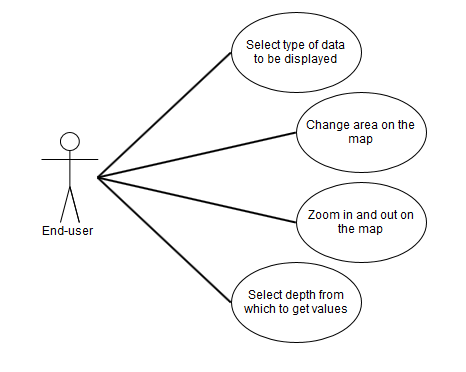
\includegraphics[height=125px,width=186px]{img/useCase_EndUser.png}
	\caption{End-user Use Case Diagram}
	\label{fig:endUserUseDiagram}
	%\medskip
	\small
	\end{center}
  \end{figure}

  \begin{figure}[h]
	\begin{center}
	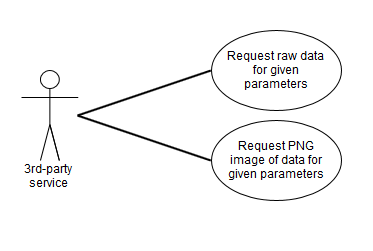
\includegraphics[height=125px,width=186px]{img/useCase_3rdParty.png}
	\caption{3rd-party Use Case Diagram}
	\label{fig:3rdPartyUseDiagram}
	%\medskip
	\small
	\end{center}
  \end{figure}

    The end-user is performing actions on the \gls{front-end} part of the system, while the 3rd-party service performs its actions on the \gls{back-end} part of the system. The end-user would then again use the 3rd-party service. In the future more operations might be allowed as the system expands from its core functionality, but these have been left outside the scope for this project.

  \subsection{Use cases}
	For our \gls{pre-study}, SINTEF put forth a series of situations were their system is used by the fishery industry. 
	\begin{itemize}
		\item \textbf{Planning of new fish farm sites} \\
		When choosing a new site for a fish farm, it is important to be aware of historical information on currents, temperature and salinity. Placing a new site in an area that has high currents might make construction and other operations difficult.
		\item \textbf{Planning the removal of lice in a fish farm} \\
		In the event that lice has to be removed from the fish in the farm, there are two procedures that are used. In the first scenario, a tanker vessel will pump the fish from the farm into a holding room. Here, the fish is treated with chemicals before being pumped back to the farm. The second method brings in crane boats, that hoist the farm, thus shrinking the volume the fish has available. A canvas is then used to surround the fish, and the chemicals are added directly. 

		Both these operations require calm currents, as to ensure that any support vessels are able to stay in position during the operation. Having access to the latest current predictions is vital in the planning of this type of operation.
		\item \textbf{Planning feeding of fish in fish farms} \\
		The fish in a farm is kept in close confinement. When the fish is fed, their activity rises significantly, consuming larger amounts of oxygen than usual. Given the right combination of temperature and currents, this could lead to oxygen levels dropping to dangerously low levels. Being able to plan feeding in accordance with forecasts for temperature and currents minimizes the risk of harm to the fish.
	\end{itemize}

\section{Requirements Specification}
\label{reqspec}
We have decided to have detailed documentation on our functional requirements, as we choose to base our product backlog from them.

  \subsection{Prioritization}
  All functional requirements have been prioritized on a scale of 1 to 100 in order of importance, where 1 is the lowest priority and 100 is the highest. These priorities where set by the customer based on our input and priorities in the categories High, Medium and Low.

  \subsection{Functional Requirements}
  The functionality of the system is described through its functional requirements. Based on  conversations with the customer, use cases, and existing solutions for these use cases, it is possible to formulate the functional requirements. Below is a table listing all the functional requirements divided into tables for \gls{front-end} and \gls{back-end}. The requirements are listed with deeper explanation, priority, and a time estimate.
  \\
  \begin{longtable}{p{1.4cm} p{7.8cm} p{1cm} p{1cm} }
  \caption[]{Functional Requirements \gls{back-end}}\\
  \multicolumn{1}{p{1.4cm}}{ID} &
  \multicolumn{1}{p{7.8cm}}{Requirement Description} &
  \multicolumn{1}{p{1cm}}{Prio.} &
  \multicolumn{1}{p{1cm}}{Est.}
  \endhead

  \caption[Functional Requirements \gls{back-end}]{} \label{funcReqsBack} \\
  \hline \multicolumn{4}{c}{\textbf{Back-End}} \\
  \hline
  \multicolumn{1}{p{1.4cm}}{ID} &
  \multicolumn{1}{p{7.8cm}}{Requirement Description} &
  \multicolumn{1}{p{1cm}}{Prio.} &
  \multicolumn{1}{p{1cm}}{Est.}
  \endfirsthead
  
  \hline
  \multicolumn{4}{r}{{Continued on next page}} \\
  \endfoot

  \hline \hline
  \endlastfoot

  \hline  
  FR 1.1 & The \gls{back-end} must be able to find the correct files for a given area
  
  \begin{itemize}
  \item \parbox[t]{6.8cm}{
        Given one or more \gls{netcdf} files in the storage \\ 
        When a request for an area arrives \\ 
        Then the \gls{back-end} will return the correct files}
  \end{itemize}
   & 99 & 10h \\ \hline
  
  FR 1.2 & The \gls{back-end} must be able to find the correct files for a given time 
  \begin{itemize}
  \item \parbox[t]{6.8cm}{
        Given one or more \gls{netcdf} files in the storage \\ 
        When a request for a time is given \\ 
        Then the \gls{back-end} will return the correct files}
  \end{itemize}
  & 98 & 6h \\ \hline %estimage given FR 1.1?

  FR 1.3 & The \gls{back-end} must be able to find the correct data from a given file 
  \begin{itemize}
  \item \parbox[t]{6.8cm}{
        Given a \gls{netcdf} file \\ 
        When a request of specific parameters arrives \\ 
        Then the \gls{back-end} will return the relevant dataset from the \gls{netcdf} file}
  \end{itemize}
  & 97 & 8h \\ \hline

  FR 1.4 & The \gls{back-end} must be able to downsample data to a given resolution 
  \begin{itemize}
  \item \parbox[t]{6.8cm}{
        Given a dataset \\ 
        When it is necessary \\ 
        Then the \gls{back-end} should downsample the data to a reasonable size}
  \end{itemize}
  & 50 & 15h \\ \hline

  FR 1.5 & The \gls{back-end} must be able to handle overlapping areas and give back correct data
  \begin{itemize}
  \item \parbox[t]{6.8cm}{
        Given a set of \gls{netcdf} files in store \\
        When a request for an area that is covered by multiple files arrives \\
        Then the \gls{back-end} should return a single data set with the correct data from all relevant files}
  \end{itemize}
  & 49 & 30h \\ \hline

  FR 1.6 & The \gls{back-end} must be able to find the most up to date data
  \begin{itemize}
  \item \parbox[t]{6.8cm}{
        Given multiple \gls{netcdf} files overlapping in time \\
        When a time in this overlap is requested \\
        Then the data from the most up to date \gls{netcdf} file should be used}
  \end{itemize}
  & 48 & 6h \\ \hline

  FR 1.7 & The \gls{back-end} must be consistent and return the same output for the same input as long as no relevant files have been changed
  \begin{itemize}
  \item \parbox[t]{6.8cm}{
        Given a repeated request \\
        When no new relevant files are added \\
        Then the \gls{back-end} must return the same dataset}
  \item \parbox[t]{6.8cm}{
        Given a repeated request \\
        When new relevant files are added \\
        Then the \gls{back-end} must return the most up-to-date dataset}
  \end{itemize}
  & 47 & 10h \\ \hline

  FR 1.8 & The \gls{back-end} must return the most relevant data after new files are added to the system
  \begin{itemize}
  \item \parbox[t]{6.8cm}{
        Given a \gls{back-end} with cached results \\
        When a more up to date \gls{netcdf} file is added to the system and request arrives \\
        Then the \gls{back-end} must calculate new results instead of using the now out of date cached results}
  \end{itemize}
  & 46 & 12h \\ \hline

  FR 1.9 & The \gls{back-end} should be able to handle new files on a daily basis
  \begin{itemize}
  \item \parbox[t]{6.8cm}{
        Given a schedule of adding new files daily \\
        When the new files are added to the system \\
        Then the \gls{back-end} should process these efficiently without major disturbance to the system}
  \end{itemize}
  & 45 & 8h \\ \hline

  FR 1.10 & Administrators must be able to add files to the system
  \begin{itemize}
  \item \parbox[t]{6.8cm}{
        Given a system with an existing set of files \\
        When an administrator wants to add new \gls{netcdf} files \\
        Then the \gls{back-end} should be able to add these to the set of existing files without recompiling}
  \end{itemize}
  & 44 & 6h \\ \hline

  FR 1.11 & Files added to the system should be ready for use without any more manual actions
  \begin{itemize}
  \item \parbox[t]{6.8cm}{
        Given a system with an existing set of files \\
        When an administrator has added new \gls{netcdf} files \\
        Then the \gls{back-end} should be able to process these files and make them usable together with the existing set of files without further action from the administrator}
  \end{itemize}
  & 43 & 10h \\ \hline

  FR 1.12 & The \gls{back-end} should be able to provide correct projections of point data
  \begin{itemize}
  \item \parbox[t]{6.8cm}{
        Given a system of \gls{netcdf} files \\
        When a point is specified in world coordinates \\
        Then the \gls{back-end} should be able to correctly project this onto coordinates of the \gls{netcdf} files}
  \end{itemize}
  & 42 & 20h \\ \hline

  FR 1.13 & The \gls{back-end} should be able to provide the current direction data, given a area, time and depth
  \begin{itemize}
  \item \parbox[t]{6.8cm}{
        Given a system of files containing current direction data \\
        When a current direction request for a given area, time and depth arrives \\
        Then the \gls{back-end} should serve the current direction data for this area}
  \end{itemize}
  & 41 & 20h \\ \hline

  FR 1.14 & The \gls{back-end} should be able to provide the temperature data, given a area, time and depth
  \begin{itemize}
  \item \parbox[t]{6.8cm}{
        Given a system of files containing temperature data \\
        When a temperature request for a given area, time and depth arrives \\
        Then the \gls{back-end} should serve the temperature data for this area}
  \end{itemize}
  & 90 & 15h \\ \hline

  FR 1.15 & The \gls{back-end} should be able to provide the salinity data, given a area, time and depth
  \begin{itemize}
  \item \parbox[t]{6.8cm}{
        Given a system of files containing temperature data \\
        When a temperature request for a given area, time and depth arrives \\
        Then the \gls{back-end} should serve the temperature data for this area}
  \end{itemize}
  & 89 & 8h given FR 1.14 \\ \hline

  FR 1.16 & The \gls{back-end} should be able to provide the current data, given a area, time and depth
  \begin{itemize}
  \item \parbox[t]{6.8cm}{
        Given a system of files containing current data \\
        When a current request for a given area, time and depth arrives \\
        Then the \gls{back-end} should serve the current data for this area}
  \end{itemize}
  & 50 & 8h given FR 1.14 \\ \hline

  FR 1.17 & The \gls{back-end} should be able to provide a \gls{PNG} image for the given temperature data
  \begin{itemize}
  \item \parbox[t]{6.8cm}{
        Given a temperature dataset \\
        When requested to return the dataset in \gls{PNG} image format \\
        Then the \gls{back-end} should make a \gls{PNG} image to represent the dataset with value-color mapping relevant to temperature}
  \end{itemize}
  & 90 & 30h \\ \hline

  FR 1.18 & The \gls{back-end} should be able to provide a \gls{PNG} image for the given salinity data
  \begin{itemize}
  \item \parbox[t]{6.8cm}{
        Given a salinity dataset \\
        When requested to return the dataset in \gls{PNG} image format \\
        Then the \gls{back-end} should make a \gls{PNG} image to represent the dataset with value-color mapping relevant to salinity}
  \end{itemize}
  & 89 & 10h given FR 1.17 \\ \hline

  FR 1.19 & The \gls{back-end} should be able to provide a \gls{PNG} image for the given current data
  \begin{itemize}
  \item \parbox[t]{6.8cm}{
        Given a current dataset \\
        When requested to return the dataset in \gls{PNG} image format \\
        Then the \gls{back-end} should make a \gls{PNG} image to represent the dataset with value-color mapping relevant to current}
  \end{itemize}
  & 50 & 10h given FR 1.17  \\ \hline

  FR 1.20 & The \gls{back-end} should be able to provide current direction data in an easily usable format
  \begin{itemize}
  \item \parbox[t]{6.8cm}{
        Given a current direction dataset \\
        When it is not specifically requested to return unprocessed data \\
        Then the \gls{back-end} should convert the current direction data into an easily usable format like GeoJSON}
  \end{itemize}
  & 50 & 20h \\ \hline

  FR 1.21 & The \gls{back-end} should provide the raw data in \gls{JSON} format
  \begin{itemize}
  \item \parbox[t]{6.8cm}{
        Given some data \\
        When requested to return the raw data \\
        Then the \gls{back-end} should return it in \gls{JSON} format}
  \end{itemize}
  & 10 & 8h \\ \hline

  FR 1.22 & The \gls{back-end} should implement the \gls{WMTS}-\gls{protocol} & 95 & 30h \\ \hline

  FR 1.23 & The \gls{back-end} should implement a relevant subset of REST & 10 & 12h \\ \hline
  \end{longtable}
  
  \vspace{2cm}

  \begin{longtable}{p{1.4cm} p{7.8cm} p{1cm} p{1cm} }
  \caption[]{Functional Requirements \gls{front-end}} \\
  \hline \hline
  \multicolumn{1}{p{1.4cm}}{ID} &
  \multicolumn{1}{p{7.8cm}}{Requirement Description} &
  \multicolumn{1}{p{1cm}}{Prio.} &
  \multicolumn{1}{p{1cm}}{Est.}
  \endhead

  \caption[Functional Requirements \gls{front-end}]{} \label{funcReqsFront} \\
  \hline \multicolumn{4}{c}{\textbf{Front-End}} \\
  \multicolumn{1}{p{1.4cm}}{ID} &
  \multicolumn{1}{p{7.8cm}}{Requirement Description} &
  \multicolumn{1}{p{1cm}}{Prio.} &
  \multicolumn{1}{p{1cm}}{Est.}
  \endfirsthead

  \hline
  \multicolumn{4}{r}{{Continued on next page}} \\
  \endfoot

  \hline \hline
  \endlastfoot
  
  \hline
  FR 2.1 & The \gls{front-end} must be able to provide a map with overlaying image
  \begin{itemize}
  \item \parbox[t]{6.8cm}{
        Given a \gls{front-end} \gls{GUI} \\
        When a user loads the page \\
        Then the \gls{front-end} should provide a map and display an overlaying image on top of it}
  \end{itemize}
  & 100 & 20h \\ \hline

  FR 2.2 & The user must be able to specify area and time for the map to display
  \begin{itemize}
  \item \parbox[t]{6.8cm}{
        Given a \gls{front-end} \gls{GUI} \\
        When the user want to specify area and time
        Then the user should be able to intuitively do so in the \gls{GUI}}
  \item \parbox[t]{6.8cm}{
        Given a \gls{front-end} \gls{GUI} \\
        When the user has specified area and time
        Then the \gls{front-end} should provide the data for the given area and time}
  \end{itemize}
  & 90 & 24h \\ \hline

  FR 2.3 & The user must be able to display data from a chosen depth
  \begin{itemize}
  \item \parbox[t]{6.8cm}{
        Given a \gls{front-end} \gls{GUI} \\
        When the user wants to specify a depth \\
        Then he should be able to intuitively specify the depth in the \gls{GUI}}
  \item \parbox[t]{6.8cm}{
        Given a \gls{front-end} \gls{GUI} \\
        When user specifies a depth \\
        Then the \gls{GUI} should display the data for the given depth}
  \end{itemize}
  & 80 & 15h \\ \hline

  FR 2.4 & The user must be able to choose data type to be displayed (temperature, salinity or current)
  \begin{itemize}
  \item \parbox[t]{6.8cm}{
        Given a \gls{front-end} \gls{GUI} \\
        When the user wants to select data type \\
        Then he should be able to intuitively choose the data type in the \gls{GUI}}
  \item \parbox[t]{6.8cm}{
        Given a \gls{front-end} \gls{GUI} \\
        When the user selects a data type \\
        Then the \gls{GUI} should display the data for this selected type of data in the map}
  \item \parbox[t]{6.8cm}{
        Given a \gls{front-end} \gls{GUI} \\
        When the user requests data on temperature, salinity or current \\
        Then it is received and displayed in \gls{PNG} image format}
  \end{itemize}
  & 70 & 10h \\ \hline

  FR 2.5 & The user must be able to zoom and pan in the displayed map
  \begin{itemize}
  \item \parbox[t]{6.8cm}{
        Given a map in the \gls{front-end} \gls{GUI}
        When the user wants to zoom or pan
        THen he should be able to do so with intuitive mouse or button actions}
  \end{itemize}
  & 30 & 5h \\ \hline

  FR 2.6 & The existing data must move and scale when zooming and panning
  \begin{itemize}
  \item \parbox[t]{6.8cm}{
        Given a map in the \gls{front-end} \gls{GUI} with existing data loaded
        When the user performs a zoom or pan action
        Then the existing data should scale and move correctly}
  \end{itemize}
  & 20 & 5h \\ \hline

  FR 2.7 & New data must dynamically load when view-area is changed sufficiently
  \begin{itemize}
  \item \parbox[t]{6.8cm}{
        Given a map in the \gls{front-end} \gls{GUI} \\
        When the user zoom closer in the map to where a more detailed dataset would be needed \\
        Then the \gls{front-end} should dynamically load a more detailed dataset}
  \item \parbox[t]{6.8cm}{
        Given a map in the \gls{front-end} \gls{GUI} \\
        When the user zoom further away in the map to where not all of the view is covered by the previous dataset \\
        Then the \gls{front-end} should dynamically load new datasets on the same level of detail, or if a certain threshold is passed it should load datasets on a less detailed level}
  \item \parbox[t]{6.8cm}{
        Given a map in the \gls{front-end} \gls{GUI} \\
        When the user pan the map so that we do not have all of the view covered by the previous dataset \\
        Then the \gls{front-end} should dynamically load the datasets to cover the new view}
  \end{itemize}
  & 10 & 30h \\ \hline

  FR 2.8 & The \gls{front-end} should be able to display current directions
  \begin{itemize}
  \item \parbox[t]{6.8cm}{
        Given a \gls{front-end} \gls{GUI} \\
        When the user requests a dataset and the option for current direction is marked \\
        Then the \gls{front-end} should request the current direction dataset and display it as an overlay over the map and/or other datasets}
  \end{itemize}
  & 40 & 30h \\ \hline

  \end{longtable}

  \subsection{Non-Functional Requirements}
  We have also made a list of essential non-functional requirements. All of them are essential and will have a high priority in our project.

  \begin{longtable}{p{1.4cm} p{9.8cm} }
  \caption[Non-Functional Requirements]{Non-Functional Requirements} \label{nonFuncReqs} \\
  \hline
  \multicolumn{1}{p{1.4cm}}{\textbf{ID}} &
  \multicolumn{1}{p{9.8cm}}{\textbf{Requirement Description}}
  \endfirsthead

  \multicolumn{2}{r}{{Continued on next page}} \\
  \endfoot

  \hline \hline
  \endlastfoot

  \hline
  \gls{QA} 1.1 & The system should be easily modifiable to add new functionality\\ \hline

  \gls{QA} 1.2 & The requests must be fast enough to feel responsive for the user \\ \hline

  \gls{QA} 1.3 & The modules should be well documented and easily understandable for those who will work on it later \\ \hline

  \gls{QA} 1.4 & The \gls{API} between \gls{front-end} and \gls{back-end} should be well documented to be usable together with other \gls{front-end} or \gls{back-end} solutions \\ \hline

  \gls{QA} 1.5 & The \gls{front-end} and \gls{back-end} parts of the system should be segregated for security and ease of use separately \\ \hline

  \end{longtable}


\chapter{Pre-sprint work}
This chapter will explain how the group worked and what we did in the weeks leading up to Sprint 1.

\section{Understanding the customers problem and needs}

\paragraph{Learning about their current solution}
At our first two meetings with SINTEF we were introduced to how they currently presents data to its users and some of the problems with this solution. They also gave some examples of who their users were and why they might access the data. We were offered access to the front end of their current solution to explore on our own.

\paragraph{Agreeing on the scope of our work}
After some discussion in the group and clarifications from SINTEF, we wrote a suggestion for the scope of our task: 
\begin{quote} Make a \gls{pre-study} that examines what technology can be used to replace the current collection of PDFs, and instead serve the end user with custom visualisations on a web page. Follow the study with an implementation of a \gls{proof of concept} system that is able to read a \gls{netcdf}-file, and present data to the end user based on custom chosen variables. We will ignore any bottlenecks that may exist in SINTEFs systems, and assume that they are fixable. Our end report will contain suggestions for further development and analysis.
\end{quote}
Our contact at SINTEF accepted this with one change, that the system should be able to read from a collection of \gls{netcdf} files. The group agreed to this change.

\section{Group organization}
\paragraph{Workflow}
After some discussion and investigation the group decided to use scrum for the main part of the project. Before starting the scrum sprints proper we assigned tasks less formally. At each meeting we decided on what tasks should be done by next meeting, and divided them among us.

\paragraph{Roles and teams}
Each group member was assigned one or more areas of responsibility. The group was split into two teams to research for the pre study, one for front end and one for back end. This split will remain as the customer wants us to create both a custom front and back end.

\paragraph{Setting up tools}
The group agreed on and set up several tools to facilitate communication and work:
\begin{itemize}
	\item Slack channels for instant messaging and file sharing
	\item Google Groups for group-wide emails
	\item Git for the reports and code
	\item Google Drive for smaller documents and time tracking
	\item Trello for issue tracking
\end{itemize}

\paragraph{Project plan}
We created a project plan to outline the phases of the project. It also includes a schedule for the sprints and milestones.
	
\paragraph{\glsentryname{QA} rules}
The group agreed with the customer on time limits for scheduling meetings and email responses.

\paragraph{Risk assessment}
In order to be better prepared, we listed and assessed possible problems. We also outlined ways of minimizing the chance of the risk occurring, as well as how they might be handled if they should occur.

\section{Work on the pre study}
The main goal of the first project period was to produce a preliminary study. This presented the customer with possibilities on how the work should proceed. Based on a recommendation by the group and after some discussion, the customer made a decision. The pre study took several weeks to produce, and work focused on these tasks:

\paragraph{Documenting the current solution}
To gain a better perspective on what the customer wanted, we documented what SINTEFs current system looked like, what data it presented and how. This project aims to solve some of the challenges and limitations of the current system.

\paragraph{Researching production solutions}
In order to better understand what a modern system similar to what SINTEF wants might look like we investigated online solutions in production around the world. This also gave some insight into what technologies are most commonly used. Prompting us to look into whether these technologies could be used in our project as well.

\paragraph{Back end technologies}
The back end part of the group looked into and tested several technologies that might be useful. One of the largest problems was finding some technology to handle the aggregation of the different gridsizes in SINTEFs datasets. Our investigations revealed that no existing technology would cover our needs, at least without extensive modification. Other problems included limited support for \gls{netcdf} and difficulty configuring the programs. We created some \glspl{prototype} to learn more about how difficult a custom solution from scratch might be, and its performance.

\paragraph{Front end technologies}
Several technologies were available for presenting map data to the user. We looked into rendering the data client-side. This proved inefficient, and together with observations of other production solutions using \gls{PNG}-tiles we decided to look more into that instead. Some testing revealed OpenLayers to be the best candidate for handling the dynamic map presentation of data.

\paragraph{Recommendation and decision}
In internal discussions the group found it best to present SINTEF not with one recommendation, but a choice between two paths. For the front end, we concluded that a custom solution would be the best, because what little existed would need a lot of modification. The \gls{back-end} would either be a \gls{THREDDS} server configured by SINTEF or a custom solution. The path involving a custom back end came with the caveat that the final product might not be as feature complete, as the group would need to divide its attention.
\par Our contacts at SINTEF were presented with the findings and our recommendation. After some discussions with the group they chose the custom back end path.

\section{Other}

\paragraph{Proof of concept back end}
Early on we knew we there was a possibility of having to create or modify code accessing and serving the data from \gls{netcdf} files. In order to learn about the performance and effort involved we created some \glspl{prototype} in Java. We were quickly able to extract data from the \gls{netcdf} files, serving them as \gls{JSON} via REST or creating images.


\chapter{Sprint 1}
\paragraph{Sprint duration: 6/10-2014 until 13/10-2014} \hfill \\
\\
\noindent
This sprint marks the formal start of the implementation work. Up to this point, the group has focused mainly on the pre study, which has done an extensive study into the possible choices for the customer. In this process, \glspl{prototype} were implemented, but this was only meant for the group to get an idea of the work involved. Thus, the real work of implementation starts at this point, though the prototyping obviously will be a great help in the work ahead. 

At the same time as sprint 1 started, the final work on the pre delivery for \gls{NTNU} also had to be done. This was a lot of work, and the group decided at the start of sprint 1 to use this sprint almost exclusively for working on the pre delivery, as it is needed to be allowed to continue the course, as well as an important milestone in the project plan. 

\section{Sprint planning}
From our formalized scope and the choice the customer made based on our pre study, we created a list of requirements. The list of functional requirements will serve as our project backlog. In discussion with the group, the customer gave each requirement a priority to serve as a guideline when creating the sprint backlogs.

\section{Goal for next demo}
For our first demo, the customer wants us to, in his words, "get something up and running". More specifically, the customer wants a map showing, with an overlay of some sort. This can then be used by the customer to make decisions on how to move forward, and what to prioritize later in the project. The customer was not concerned with the system displaying real data at this point, and only wants the demo to show the general idea of the system. As we only demo for the customer every other week, this goal can be fulfilled in two weeks.

\section{Sprint backlog}
The backlog for the first sprint consisted mainly of tasks that are connected to the pre delivery. This because of the strict deadline this delivery has, as well as the need for everyone to work on the pre delivery to ensure that it would be done on time.

The following tasks where committed to in sprint 1:

\begin{description}
	\item[Reporting] \hfill \\ 
	Write requirements for \gls{pre-delivery} \hfill \\
	Write project plan for \gls{pre-delivery} \hfill \\
	Write introduction and abstract for \gls{pre-delivery} \hfill \\
	Write technology chapter for \gls{pre-delivery} \hfill \\
	Write project planning section for \gls{pre-delivery} \hfill \\
	Write risk assessment for \gls{pre-delivery} \hfill \\
	Write weekly documents for advisor meeting
\end{description}

For this sprint, the group chose not to estimate the tasks. This decision was done in part because it is inherently difficult to estimate time for writing, but also because the team knew that these tasks had to be done by the end of the sprint. This meant that whether or not the estimates would exceed the limit on work hours, the work had to be done.

\section{Sprint overview}
The sprint was focused on the \gls{pre-delivery} for \gls{NTNU}. While this does not directly add value to the customer, the team has to ensure that all required documents are handed in on time. Failing to meet this deadline would lead to the team failing the course, and the customer obviously has an interest in the team being allowed to continue their work. 

During this sprint, the \gls{pre-delivery} was almost finished. All team members where able to finish their parts, and only small corrections, as well as making the document consistent remains. 

\section{Evaluation}
The group was able to finish most of the \gls{pre-delivery} tasks for the first sprint. This was vital in being able to advance the project. Writing a lot for the report was in some respects challenging. The team had to divide the writing in to a lot of subtasks. Since every team member has their own writing style, all the text has to be looked over by one person afterwards, to correct inconsistencies, and to do a quality assurance of the work. This work is left for the next sprint. For some of the team members, focusing solely on reporting was not very motivating, as the group has been waiting for the opportunity to start coding. Non the less, almost all work in the sprint was completed.

After the sprint finished, there was work left in the following tasks:

\begin{description}
	\item[Reporting] \hfill \\ 
	Write requirements for \gls{pre-delivery} \hfill \\
	Write introduction and abstract for \gls{pre-delivery} \hfill \\
\end{description}

The remaining work on the requirements is mainly \LaTeX-formating. The introduction is still lacking in some areas. This is because some sections has to be written last, and due to some lack of time. The group does not think it will be a problem to finish this in the next sprint. 

\chapter{Sprint 2}
\paragraph{Sprint duration: 13/10-2014 until 20/10-2014} \hfill \\
\\
\noindent
Sprint 2 will be the first sprint the group can focus on implementation work. As the next customer demo is the Wednesday after the sprint ends, the goal for the demo has to be achieved in this sprint. The customer has stated that their goal is for us to "get something up and running". In choosing tasks for this sprint, the group has kept this goal in mind. 

\section{Sprint planning}
We have had a meeting discussing the use of time for the project, and it seems as if not all group members are using their full 25 hours a week. Because of this, the decision was made to be stricter in both estimation and assignment of tasks for this sprint. Based on the experiences from last sprint, it seems as if there is a higher threshold for group members to take on a new task in the middle of a sprint, than to take on more tasks at the start. It will then be better to assign to many tasks, and then have work left, than to assign to few, and thus have unused resources. 

\section{Sprint backlog}
The sprint backlog was in this sprint split into three sections. This represents the different work that has to be done, and also the way the group has decided to split the work. The \gls{pre-delivery} is due on the friday of this sprint. The group has assigned two people to work on the remaining tasks for this, and the rest of the group will start on the implementation work. 

\begin{description}
	\item[Front end] \hfill \\
	Get a map up and running
	\item[Back end] \hfill \\
	Handle projections \hfill \\
	Image output module \hfill \\
	Parse parameters to select region \hfill \\
	Implement feature endpoints \hfill \\
	Implement vector feature endpoints \hfill \\
	Set up server
	\item[Reporting] \hfill \\ 
	Write requirements for \gls{pre-delivery} \hfill \\
	Write introduction and abstract for \gls{pre-delivery} \hfill \\
	Proof-read \gls{pre-delivery} 
	Write weekly documents for advisor meeting
\end{description}
	
We have chosen to use the quite vague goal of the customer as the only task for the front end. This has the consequence of setting a task that is a lot larger than one work day. Despite of this, since the task is vague, we found it difficult to split it further. For the back end side of the project, the tasks are much more specific.

\section{Sprint overview}
The sprints focus was split in two, with most of the group working on the implementation, as to be able to demo for the customer next week. The other part of the group focused on the \gls{pre-delivery}. This separation of responsibility was done with the goal of being able to work in parallel with two important tasks that both had to finished this sprint. By dividing the group into smaller sub-groups, the tasks are perceived to be the responsibility of fewer people, and the team members are more likely to step up and go the extra mile when needed. 

\section{Evaluation}
The most important part of this sprint was to be able to hand of the \gls{pre-delivery} on time. This was done, and the group is happy with the result. All required parts of the \gls{pre-delivery} was finished, and there was time for most of the group to proof read the delivery. The group is also prepared to give the customer a demo of the system next week. At this point, the system has a working front end, which makes requests to the back end in accordance to the \gls{WMTS} \gls{protocol}. The back end is able to read a single \gls{netcdf} file, and output an image that is transferred to the front end, and displayed on the map. This is shown in figure \ref{fig:UIAfterSprint2}.

\begin{figure}[h]
\begin{center}
\fbox{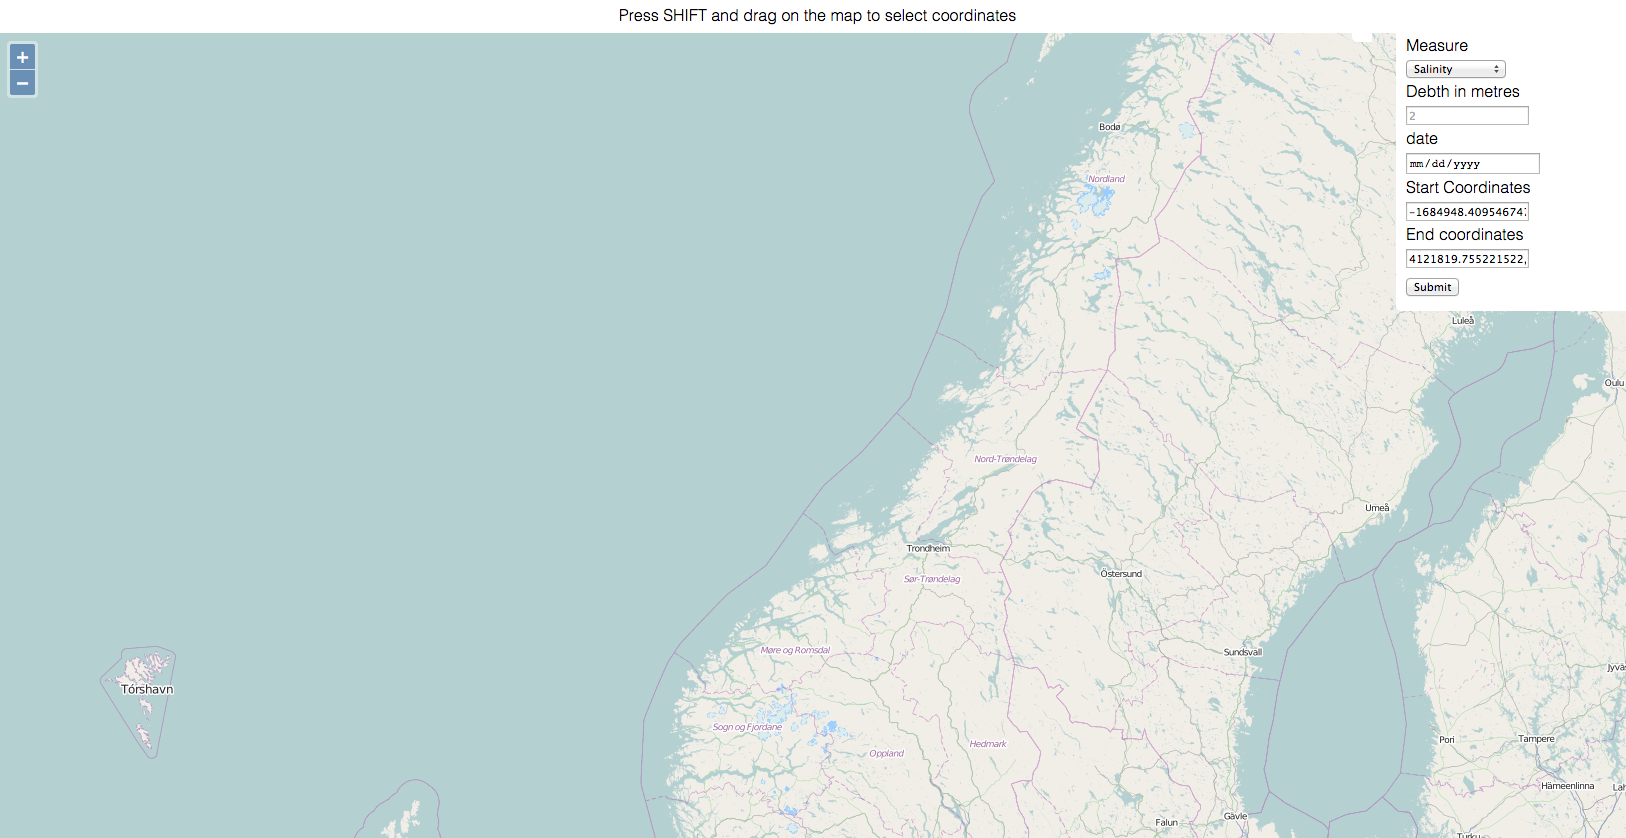
\includegraphics[height=300px,width=400px]{img/MapUI_V1.png}}
\caption{The user interface, after the completion of sprint 2}
\label{fig:UIAfterSprint2}
\end{center}
\end{figure}

The position of the overlay on the map is not completely correct, but the customers initial goal for this demo was just having a map up and running. To make sure that the demo is well prepared, one team member has been given the responsibility to plan the demo. 

As for the sprint backlog, the following items has remaining work after this sprint:

\begin{description}
	\item[Back end] \hfill \\
	Handle projections \hfill \\
	Implement feature endpoints \hfill \\
	Implement vector feature endpoints
\end{description}

All in all, the group is satisfied with the work done in the sprint. There is remaining work in the back end, but this should be possible to finish during the next sprint. Assigning one person to read trough the \gls{pre-delivery} made the language much more concise than it was initially, as well as adding a layer of quality assurance. 



\chapter{Sprint 3}
\paragraph{Sprint duration: 20/10-2014 until 27/10-2014} \hfill \\
\\
\noindent
After handing in the \gls{pre-delivery}, the group is now free to focus their efforts on the implementation. For this sprint, a demo is planned for the customer. This will hopefully give valuable feedback on both design decisions, as well as what to focus on in the implementation work.

\section{Sprint planning}
As implementation is the main activity of this sprint, the group has assigned all but one group member to work on implementation. The group at large will focus on improving the system, and making sure that the front end is adapted to fit the customers need. The last team member will work on the report, and make sure that the sections on the sprints are done, as well as producing internal documents. As the final report is to be handed in just days after the last sprint, it is important not to forget or neglect these tasks. 

\section{Sprint backlog}
This sprint is focused mostly on the back end work. As we will have feedback from the customer in the middle of the sprint, there might be some new tasks added to the front end part of the backlog. The customer has in meetings with the group said that they will probably have input on the front end, especially the user interface. The sprint backlog is given in table \ref{tab:Sprint3Backlog}. It can be seen that not all tasks have been estimated. Some of these tasks where deemed too difficult to estimate, while some was not estimated when they where picked by a team member in the middle of the sprint. 

\begin{table}[h]
\centering
\resizebox{\textwidth}{!}{%
\begin{tabular}{llll}
\hline
Task                                                                                            & \begin{tabular}[c]{@{}l@{}}Estimated\\ remaining hours\end{tabular} & \begin{tabular}[c]{@{}l@{}}Actual\\ hours\end{tabular} & Assigned to   \\ \hline
\rowcolor[HTML]{C0C0C0} 
\multicolumn{4}{l}{\cellcolor[HTML]{C0C0C0}\textbf{Front end}}                                                                                                                                                                                 \\
Enable user to display data from chosen time                                                    & -                                                                   &                                                        & Anders        \\
Enable user to display data from chosen depth                                                   & 15                                                                  & 6                                                      & Anders        \\
Enable user to pan and zoom in the displayed map                                                & 15                                                                  & 3                                                      & Marco         \\
Existing data must zoom and pan with the map                                                    & 5                                                                   & 1                                                      & Ruben         \\
\rowcolor[HTML]{C0C0C0} 
\textbf{Back end}                                                                               &                                                                     &                                                        &               \\
Handle projections                                                                              & -                                                                   & -                                                      & Arve          \\
Implement feature endpoints                                                                     & -                                                                   & 7                                                      & Arve, Ondrej  \\
Implement vector feature endpoint                                                               & 5                                                                   &                                                        & Ondrej        \\
Implement WMTS                                                                                  & -                                                                   & 2,5                                                    & Arve          \\
\begin{tabular}[c]{@{}l@{}}Choose correct file based on selected\\ region and time\end{tabular} & -                                                                   & 17                                                     & Emil          \\
Handle overlapping areas                                                                        & 30                                                                  & 3                                                      & Arve, Ondrej  \\
Design WMTS architecture                                                                        & 16                                                                  & 2                                                      & Arve, Ruben   \\
Deploy script for server                                                                        & 4                                                                   & 4                                                      & Arve          \\
\rowcolor[HTML]{C0C0C0} 
\multicolumn{4}{l}{\cellcolor[HTML]{C0C0C0}{\color[HTML]{333333} \textbf{Reporting}}}                                                                                                                                                          \\
Tidy up pre-delivery parts of report                                                            & 4                                                                   & 12                                                     & Hans Kristian \\
Make sprint template                                                                            & 3                                                                   & 3                                                      & Hans Kristian \\
Write sprint 1                                                                                  & 3                                                                   &                                                        & Hans Kristian \\
Wirte sprint 2                                                                                  & 3                                                                   &                                                        & Hans Kristian \\
Write weekly documents for advisor meeting                                                      & 3                                                                   & 2                                                      & Hans Kristian \\
\rowcolor[HTML]{C0C0C0} 
\textbf{Total}                                                                                  & 106                                                                 & 62,5                                                   &              
\end{tabular}
}
\caption{Sprint 3 Backlog}
\label{tab:Sprint3Backlog}
\end{table}

\section{Sprint overview}
This sprint is more focused on the back end than the front end. In the back end, there are more tasks that has to be completed, and these do not require direct feedback from the customer. For the front end, tasks that involve sending correct requests to the back end, and functionality that has to be implemented regardless of the customers feedback has been chosen. 
\section{Evaluation}
\paragraph{Sick customer}
During this sprint, the group was supposed to have their first demo for the customer. The group had planned on getting feedback on the user interface, and feedback on the customers view of the progress. Unfortunately, the customer fell ill, and was unable to meet the group. To make matters worse, none of the other employees at SINTEF that are involved with the project was able to meet the group. This meant that the group did not get any feedback on their solution in this sprint. As a consequence of this, the work on the user interface is paused until the customer is able to meet the group. 

\paragraph{Reprioritization of backlog}
Another consequence of the customer being ill and unable to meet the group, is that the backlog can not be reprioritized by the customer. It is normal for the customer to be able to make changes in the priorities in the backlog after each sprint. As the group has chosen to demo for the customer only after every other sprint, the goal was for the customer to do reprioritization after each demo. The group had to make assumptions on the customers wishes and needs to continue their work. This is not ideal, as the group may not have enough information to make these decisions, but it is better than stalling work completely. 

\paragraph{Projections}
During the work on the back end, the group has encountered quite a major problem. The problem pertains to map projections, and making the data in the \gls{netcdf} files compatible with the map we are using on the web page. Currently, the data in the \gls{netcdf} files are in the polar stereographic projection, while the map used on the page can not be set to this projection. The team is currently looking into several ways of fixing this:

\begin{description}
\item[Conversion of coordinates] It is possible to convert coordinates between different projections. This will require both a conversion factor, as well as interpolation of data. It is no trivial task, but there are well known methods for this. The main drawback for this solution is that it will be time consuming. 
\item[Conversion of \gls{netcdf}] If the entire \gls{netcdf} file is converted into the projection of the map, the problem will be solved. This will require either a program that is capable of doing the conversion, or writing such a tool from scratch. The latter seems unrealistic at this stage in the project.
\item[Replace map] The easiest solution to the problem is probably to replace the map used on the web page with a map in the correct projection. The group has already made attempts at finding a map with the correct projection, but so far this has not been successful.
\end{description}

For a full discussion on projections, and the challenges faced by the team in this area, see section \ref{sec:ProjectionChallenges}. 

\paragraph{Time usage}
As can be seen in table \ref{tab:Sprint3Backlog}, the team did not spend the required amount of time for this sprint. The backlog table does not fully reflect the time used, as most team members have not been logging their hours as thoroughly as they should have. A further discussion of this can be found in section \ref{subsec:TimeUsed}.

\paragraph{Remaining backlog items}
After the conclusion of the sprint, the following items remains in the backlog:
\begin{description}
	\item[Front end] \hfill \\
	Enable user to display data from chosen time
	\item[Back end] \hfill \\
	Implement vector feature endpoints \hfill \\
	Implement \gls{WMTS} \gls{protocol} \hfill \\
	Choose correct file based on selected region and time \hfill \\
	Handle overlapping areas 
	\item[Reporting] \hfill \\
	Write sprint 1 \hfill \\
	Write sprint 2
\end{description}

Even though the group has had an increased focus on estimation, this sprint was not completed as planned. This is in large because of the problems faced with projections. Until this is solved, a lot of other tasks also has to be placed on hold. This is true for the front end task remaining, as well as handling overlapping areas and choosing the correct files. For the reporting, tidying up the \gls{pre-delivery} proved to be a bigger task than first thought. This pushed writing about sprint 1 and sprint 2 to the next sprint.  

While the group is not satisfied with the fact that all tasks could not be completed, there is a good explanation for this. The group is hopeful that a solution to the projection problem will be found, thus enabling the group to advance with the project. 

\chapter{Sprint 4}
\paragraph{Sprint duration: 27/10-2014 until 3/11-2014} \hfill \\
\\
\noindent
This sprint will focus on getting the map projections working. This is critical in being able to finish the product, and it is also blocking several other tasks. As for the reporting, writing about the sprints will be the main focus. 

\section{Sprint planning}
With the problems relating to projections, the team will use a lot of resources trying to solve this in the current sprint. We will also try to arrange a customer meeting this week, if the customer is back on his feet at some point during the week. The reporting work will be handled mostly by one person, as we need as much resources as possible to solve the projection challenges. 
\section{Sprint backlog}
Based on what was left from the last sprint, and the priorities of this sprint, the sprint backlog for sprint 4 is reflected in table \ref{tab:Sprint4Backlog}.

\begin{table}[h]
\resizebox{\textwidth}{!}{%
\begin{tabular}{llll}
\hline
Task                                                                                                 & \begin{tabular}[c]{@{}l@{}}Estimated\\ remaining hours\end{tabular} & \begin{tabular}[c]{@{}l@{}}Actual\\ hours\end{tabular} & Assigned to         \\ \hline
\rowcolor[HTML]{C0C0C0} 
\multicolumn{4}{l}{\cellcolor[HTML]{C0C0C0}\textbf{Front end}}                                                                                                                                                                                            \\
Enable user to display data from chosen time                                                         & -                                                                   & 3                                                      & Anders              \\
\rowcolor[HTML]{C0C0C0} 
\multicolumn{4}{l}{\cellcolor[HTML]{C0C0C0}\textbf{Back end}}                                                                                                                                                                                             \\
\begin{tabular}[c]{@{}l@{}}Find background map in \\ polar stereographic projection\end{tabular}     & -                                                                   & -                                                      & Anders              \\
\begin{tabular}[c]{@{}l@{}}Investigate conversion from\\ polar stereographic projection\end{tabular} & -                                                                   & -                                                      & Emil                \\
Code refactor                                                                                        & 4                                                                   & -                                                      & Arve                \\
Scanning and indexing files                                                                          & 25                                                                  & 6,5                                                    & Emil                \\
Implement vector feature endpoint                                                                    & 5                                                                   & -                                                      & Ondrej              \\
Implement \gls{WMTS} \gls{protocol}                                                                              & 35                                                                  & 18                                                     & Arve                \\
\begin{tabular}[c]{@{}l@{}}Choose correct fiels based on \\ selected region and time\end{tabular}    & 20                                                                  & 5                                                      & Emil                \\
Handle overlapping areas (Blocked)                                                                   & 30                                                                  & 2                                                      & Arve, Ondrej        \\
\rowcolor[HTML]{C0C0C0} 
\multicolumn{4}{l}{\cellcolor[HTML]{C0C0C0}{\color[HTML]{333333} \textbf{Reporting}}}                                                                                                                                                                     \\
Write sprint 1                                                                                       & 3                                                                   & 4                                                      & Hans Kristian       \\
Wirte sprint 2                                                                                       & 3                                                                   & 4                                                      & Hans Kristian       \\
Write sprint 3                                                                                       & 3                                                                   & 4                                                      & Hans Kristian       \\
Write weekly documents for advisor meeting                                                           & 3                                                                   & 2                                                      & Hans Kristian, Emil \\
\rowcolor[HTML]{C0C0C0} 
\textbf{Total}                                                                                       & 131                                                                 & 48,5                                                   &                    
\end{tabular}
}
\caption{Sprint 4 backlog}
\label{tab:Sprint4Backlog}
\end{table}

The backlog reflects that a lot of tasks had to pushed in the last sprint, as well as the addition of new tasks to find a solution to the projection challenges. The estimates and actual hours are not complete in the backlog table. For a discussion on this, see section \ref{sec:Sprint4Evaluation}.

\section{Sprint overview}
This sprint is focused towards solving the projection challenge. The team can not complete their solution unless this problem is solved. As there are multiple ideas to solving this, the group is optimistic that one of these will be successful. The biggest unknown in this sprint is the amount of time needed for the investigation of solutions. If one of the suggested solutions quickly proves to be efficient, other investigation work can be aborted, and work on the remaining tasks can resume. If not, the group faces using large parts of this sprint investigating different solutions.

\section{Evaluation}
\label{sec:Sprint4Evaluation}
\paragraph{Customer meeting}
The group was able to set up a meeting with SINTEF representatives at the end of the sprint. Our main contact was unable to meet us, but as both the representatives have been present in most of the meetings, this did not pose any problems. 

In the meeting, the customer gave useful feedback on the design decisions made for the front end. Although it is not very user friendly to enter the coordinates by hand, some users might want to, so this functionality is kept. The customer also gave some general input on the organization of the user interface. The group will use this feedback to improve the user interface in the next sprint. 

The customer was informed that the group has hit a problem with the different projections. The customer gave some additional insight into the projections used by SINTEF. This is quite a rare projection, as it is not a standard polar stereographic projection, and the customer does not think that finding a corresponding map will be likely. The customer gave three suggestions on how to handle this:
\begin{itemize}
\item \textbf{Pixel by pixel sampling} This solution would require the extraction of a single point at the time from the \gls{netcdf} file. This way, retrieving the data for an area might result in thousands of operations. This might be a quite slow solution, but it will probably be quite easy to implement.
\item \textbf{Convert \gls{netcdf} file to new projection} Using a library by the Norwegian Meteorological Institute called \gls{Fimex}, it might be possible to convert the entire \gls{netcdf} file to the correct projection. 
\item \textbf{Area conversion with Proj.4} Using a library called Proj.4, the customer thinks it might be possible to convert a specific area to the correct projection. This will have to be investigated by the group.
\end{itemize}

Doing the conversion on the clients machine was discussed, but this is not optimal, as we do not want the client to have to do much work. This is especially important when keeping in mind that a mobile version of the product is a natural next step for the customer after the group has finished their work.

\paragraph{Projections}
The group has not been able to solve the projection problem in this sprint. After the customer meeting, the search for a map in the correct projection was aborted, as the customer does not think it will be possible to find. In addition, polar stereographic maps only cover half the globe, which makes them unattractive for map applications. 

The research into Porj.4 has been more promising. Converting 1 million points is done in about 1 second. This allows for a 1000 by 1000 pixel area to be converted in one second, which would be within the customers demand for a responsive application. Unfortunately, the data still has to be interpolated, and this might be more work than the group has time to do.

\gls{Fimex} also looks promising, but the group has yet to get it up and running. If it is able to convert the files, the group feels that this should be chosen as the solution to the projection problem. This way, efforts can be directed at finishing as much functionality as possible. 

\paragraph{User interface}
The user interface has been improved in accordance with the input given by the customer. Since the group was prepared for the customer to have input on the look of the user interface, the code was written to be easily changeable. This paid of in implementing these changes. The user interface as it is at the end of sprint 4 is shown in figure \ref{fig:UIAfterSprint4}.

\begin{figure}[t]
\begin{center}
\fbox{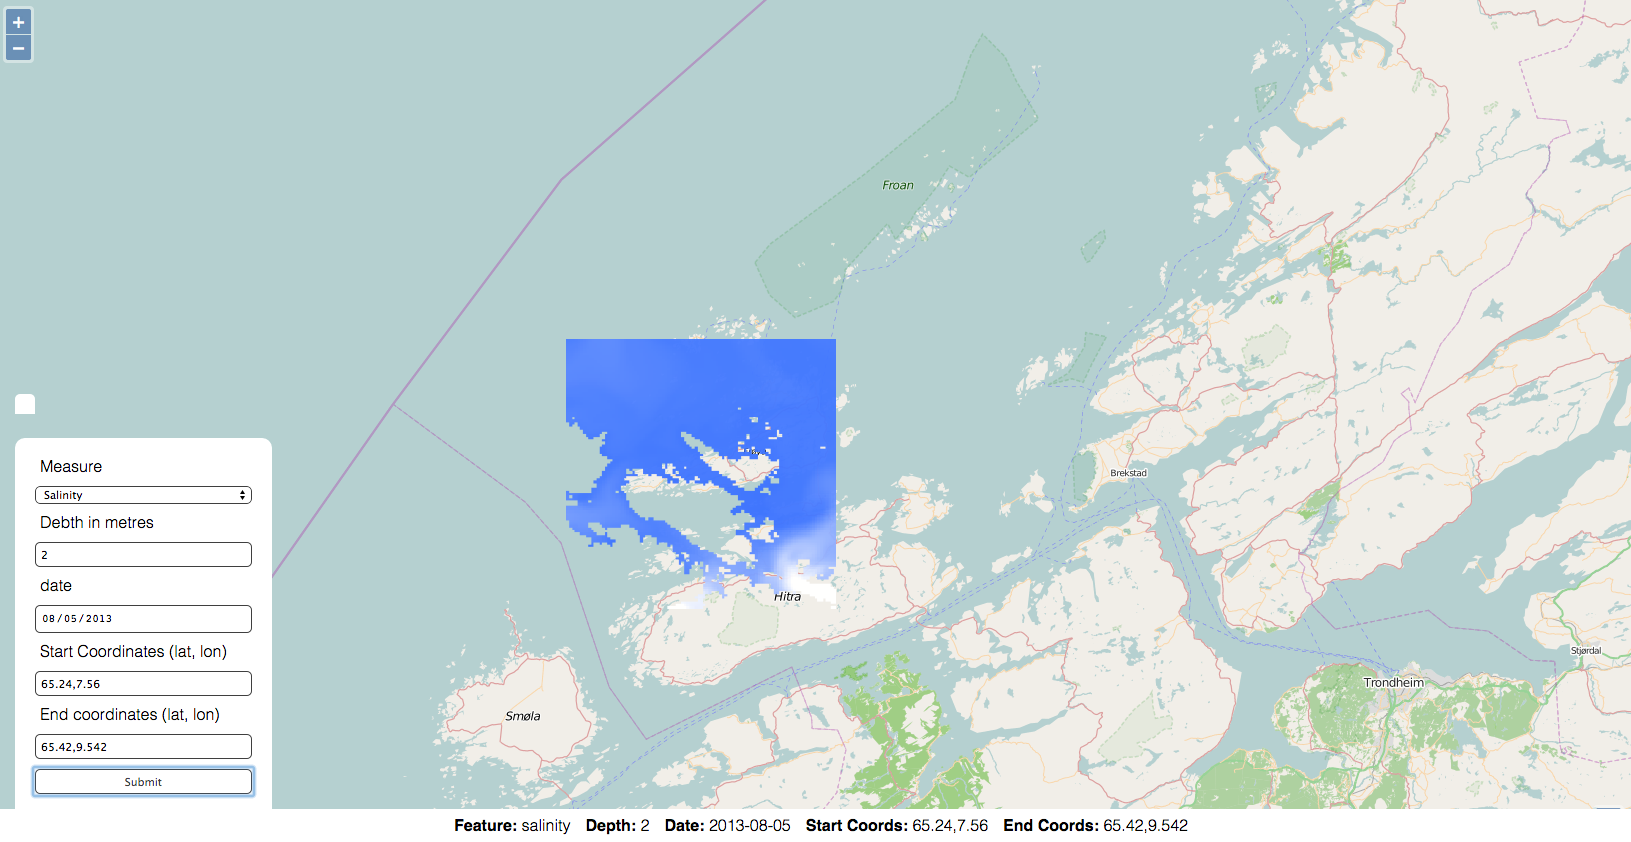
\includegraphics[height=300px,width=400px]{img/MapUI_V2.png}}
\caption{The user interface, after the completion of sprint 4. The overlay is not placed correctly due to projection challenges.}
\label{fig:UIAfterSprint4}
\end{center}
\end{figure}

\paragraph{Estimations and time usage}
The team had until this point not focused enough on time estimations and time logging. This is reflected in table \ref{tab:Sprint4Backlog} which is not complete. This is due to the fact that not all sprint items where estimated, and that not all team members did detailed time logging. Thus, the given hours spent does not reflect actual time usage. For a further discussion on the time usage in the project, see section \ref{subsec:TimeUsed}.

\paragraph{Remaining backlog items}
The items remaining in the backlog after the completion of sprint 4 are:

\begin{description}
	\item[Front end] \hfill \\
	Enable user to display data from chosen time (Blocked)
	\item[Back end] \hfill \\
	Handle projections \hfill \\
	Scanning and indexing files \hfill \\
	Implement \gls{WMTS} \gls{protocol} \hfill \\
	Choose correct file based on selected region and time \hfill \\
	Handle overlapping areas (Blocked)
\end{description}
This sprint has, as sprint 4, been focused on fixing the projection challenge. The team has made more progress in this sprint than in sprint 3, but there is still a long way to go. Unfortunately, there is not much time left in the project, and finding a solution in the next sprint is critical. Without the projections, the team will not be able to present a working \gls{prototype}. On the other hand, given that the problem is solved, the team will quite quickly have a \gls{prototype} that is able to read from the \gls{netcdf} files. 

\chapter{Sprint 5}
\paragraph{Sprint duration: 3/11-2014 until 10/11-2014} \hfill \\
\\
\noindent
This will be the penultimate sprint in the project. The group is currently in a situation where a single problem is blocking a lot of the progress. Almost all resources have been redistributed to focus on this problem. In addition to working on this, the group also has to move more resources to the report. 

\section{Sprint planning}
Until this point, one person has typically been assigned each sprint to work on the report. The exception has obviously been when finishing the \gls{pre-study}, and the \gls{pre-delivery}. For this sprint, team members are to start documenting those parts of the project they have been involved with. 

\section{Sprint backlog}
\label{sec:Sprint5Backlog}
With the tasks carried over from the last sprint, this sprint backlog is as shown in table \ref{tab:Sprint5Backlog}.

\begin{table}[h]
\resizebox{\textwidth}{!}{%
\begin{tabular}{llll}
\hline
Task                                                  & \begin{tabular}[c]{@{}l@{}}Estimated\\ remaining hours\end{tabular} & \begin{tabular}[c]{@{}l@{}}Actual\\ hours\end{tabular} & Assigned to   \\ \hline
\rowcolor[HTML]{C0C0C0} 
\multicolumn{4}{l}{\cellcolor[HTML]{C0C0C0}\textbf{Front end}}                                                                                                                                       \\
Add color legend to user interface                    & 5                                                                   &                                                        & Anders        \\
Enable user to display data from chosen time          & 10                                                                  & 7                                                      & Anders, Marco \\
\rowcolor[HTML]{C0C0C0} 
\multicolumn{4}{l}{\cellcolor[HTML]{C0C0C0}\textbf{Back end}}                                                                                                                                        \\
Investigate \gls{Fimex} and Porj.4                          & 14                                                                  & 27,5                                                   & Marco, Ruben  \\
Scanning and indexing files                           & 20                                                                  & 1                                                      & Emil          \\
Implement \gls{WMTS} \gls{protocol}                               & 15                                                                  & 21                                                     & Arve          \\
Choose correct file based on selected region and time & 10                                                                  & 1                                                      & Emil          \\
Handle overlapping areas                              & 10                                                                  & 1,5                                                    & Arve, Ondrej  \\
\rowcolor[HTML]{C0C0C0} 
\multicolumn{4}{l}{\cellcolor[HTML]{C0C0C0}\textbf{Reporting}}                                                                                                                                       \\
Add time usage to report                              & 10                                                                  & 1                                                      & Hans Kristian \\
Wirte sprint 5                                        & 3                                                                   & 4                                                      & Hans Kristian \\
Write sprint 6                                        & 3                                                                   & 2,5                                                    & Hans Kristian \\
Start final evaluation chapter                        & 10                                                                  & 10,5                                                   & Hans Kristian \\
Outline technical documentation                       & 15                                                                  & 5                                                      & Everyone      \\
Write weekly documents for advisor meeting            & 3                                                                   & 1,5                                                    & Hans Kristian \\
\rowcolor[HTML]{C0C0C0} 
\textbf{Total}                                        & 128                                                                 & 83,5                                                   &              
\end{tabular}
}
\caption{Sprint 5 backlog}
\label{tab:Sprint5Backlog}
\end{table}

The backlog has few added items for the technical side of the project. The group sees no reason to add more than necessary at this point of the project. If the projection issues are solved, there is still plenty work remaining in the sprint to keep group members busy. The reporting part of the backlog is increasing in size as the project nears the end. This is to be expected, as more and more work is now finishing, and there is thus more to write about. 

\section{Sprint overview}
Sprint 5 focuses on finding a solution to the projection problem, using the proposed solutions from the last customer meeting. In addition, the group will have to finish outlining most of the report, and preferably finish writing as many sections as possible. The team has agreed to have a meeting with the customer in this sprint to be able to show their work to the main contact at SINTEF. In addition, there is hope that the teams experience with Proj.4 and \gls{Fimex} can help start some useful discussions with the customer. With the combined knowledge of the team and customer, it might be easier to chose the right way forward. 

\section{Evaluation}
\label{sec:Sprint5Evaluation}
\paragraph{Customer meeting}
In this sprint, the group had their penultimate customer meeting. The teams progress and challenges were discussed. The group gave the customer a status report on the development, and recommended that the scope of development should be limited to the following:

\begin{itemize}
\item Basic map functionality
\item Working projections
\item Handling overlapping areas
\end{itemize}

The customer agreed that this would be a good limitation of the scope. For the functionality that can not be completed, the customer feels that there will be a lot of value in a description of this in the final report. Even though a full implementation would have been nice, the customer can benefit a lot from the groups research, and asks that as much information as possible is added to the final report. 

The team and the customer had a discussion on different ways of solving the projection issue. At the moment, the group is testing two different solutions. One will mathematically convert the coordinates of the \gls{netcdf} files to the correct projection as they are retrieved. The other will make a new \gls{netcdf} file in the same projection as the map. Then, the system can use standard methods to get the information from the \gls{netcdf} files. 

The customer does not have any preferences on how this is solved. While doing a full conversion of the \gls{netcdf} files might take some time, it will be an operation that has to be conducted only once. The customer will not have problems storing the converted files alongside the original files. 

\paragraph{Converting netCDF files}
The team has investigated the possibility of converting the entire \gls{netcdf} file, instead of converting only the coordinates of the data being retrieved, as discussed in the last customer meeting (see section \ref{sec:Sprint4Evaluation}). This solution looks promising, and the team has now been able to use the library to convert a file. At the moment, it seems to convert the data correctly, but the new \gls{netcdf} file is missing some headers. This could be the fault of the configuration file. If this is the case, and this can be easily fixed, then the system should be able to read correct data from a \gls{netcdf} file very soon.

\paragraph{Time logging}
To be able to keep track of the time used, the team agreed early that every team member would log their own time usage throughout the project. In this sprint, that material has been collected, so it can be collated and used for the report. 

It turns out that most team members have not done this logging on a regular basis, and have failed to register a lot of work effort. In addition to this, most team members have not logged time in relation to specific tasks, but rather whether the work was conducted in relation to meetings or implementation. This will make it difficult to give a correct picture of how much time has been used for different activities. Nonetheless, the group will attempt to find out how much time was used, and for what. For a more detailed discussion on time usage, see section \ref{subsec:TimeUsed}.

\paragraph{Report writing}
The final report is a large part of the basis on which the group will be evaluated. Due to the difficulties in implementing the projections correctly, there has been little time to focus on the report. This should now become a priority. The customer has made it clear that a well written report can be just as useful as a fully working product, and the group advisor has asked the group to focus on writing about features that can not be implemented on time. 

\paragraph{Remaining backlog items}
As this sprint has been mostly focused towards fixing the projection issues, not a lot of backlog items have been completed. Most of the work has been done investigating \gls{Fimex} and Proj.4. A lot of reporting has been done, though most of the technical information is still lacking from the report. 

After this sprint, the following items remain in the backlog:

\begin{description}
	\item[Front end] \hfill \\
	Add color legend to user interface \hfill \\
	Enable user to display data from chosen time (Blocked)
	\item[Back end] \hfill \\
	Investigate \gls{Fimex} and Porj.4 \hfill \\
	Handle projections \hfill \\
	Scanning and indexing files \hfill \\
	Implement \gls{WMTS} \gls{protocol} \hfill \\
	Choose correct file based on selected region and time \hfill \\
	Handle overlapping areas (Blocked)
	\item[Reporting] \hfill \\
	Add time usage to report
\end{description}

\chapter{Sprint 6}
\paragraph{Sprint duration: 10/11-2014 until 17/11-2014} \hfill \\
\\
\noindent
Sprint 6 will be the final sprint of the project. After almost three months, the project is coming to an end. In this sprint, the main focus will be finishing the report, as well as attempting to implement some last features to the solution. Hopefully, one of the investigated projection solutions can be implemented, so that the system is at least reading and displaying the data correctly.
\section{Sprint planning}
For the last sprint, the team will work mainly on the report. Every team member will be writing technical documentation on the implementations they have worked on. In addition to this, the time usage and final evaluations will be added to the report. At the end of this sprint, the report should be finished. This will give the team a day to proof read it before printing. 

In addition to writing, some team members have gotten some time to try to implement the \gls{Fimex} solution discussed in section \ref{sec:Sprint5Evaluation}. This will be the last attempt at getting the projections working. 

\section{Sprint backlog}
\label{sec:Sprint6Backlog}
The sprint backlog for this sprint contains all remaining items from the last sprint. Most of this is implementation tasks, and they will only be done if the report is finished. A lot of backlog items have been added for reporting. The total backlog can be found in table \ref{tab:Sprint6Backlog}.

\begin{table}[h]
\centering
\resizebox{\textwidth}{!}{%
\begin{tabular}{llll}
\hline
Task                                                   & \begin{tabular}[c]{@{}l@{}}Estimated\\ remaining hours\end{tabular} & \begin{tabular}[c]{@{}l@{}}Actual \\ hours\end{tabular} & Asigned to                 \\ \hline
\rowcolor[HTML]{C0C0C0} 
\multicolumn{4}{l}{\cellcolor[HTML]{C0C0C0}\textbf{Front end}}                                                                                                                                                      \\
Add color legend to user interface                     & 5                                                                   &                                                         & Anders                     \\
Enable user to display data from chosen time (Blocked) & 10                                                                  &                                                         & Anders                     \\
\rowcolor[HTML]{C0C0C0} 
\multicolumn{4}{l}{\cellcolor[HTML]{C0C0C0}\textbf{Back end}}                                                                                                                                                       \\
Investigate \gls{Fimex} and Porj.4                           & 4                                                                   &                                                         & Marco                      \\
Investigate \gls{Fimex} headers not working                  & 3                                                                   &                                                         & Marco                      \\
Make file stitching work                               & 20                                                                  &                                                         & Ondrej                     \\
Scanning and indexing files                            & 15                                                                  &                                                         & Emil                       \\
Implement \gls{WMTS} \gls{protocol}                                & 8                                                                   &                                                         & Arve                       \\
Choose correct file based on selected region and time  & 5                                                                   &                                                         & Emil                       \\
Handle overlapping areas (Blocked)                     & 10                                                                  &                                                         & Arve, Ondrej               \\
\rowcolor[HTML]{C0C0C0} 
\multicolumn{4}{l}{\cellcolor[HTML]{C0C0C0}\textbf{Reporting}}                                                                                                                                                      \\
Add time usage to report                               & 8                                                                   &                                                         & Hans Kristian              \\
Write about resources                                  & 2                                                                   &                                                         & Ondrej                     \\
Write high level architecture - Back end               & 3                                                                   &                                                         & Arve                       \\
Write about \gls{WMTS} (Challenges)                          & 3                                                                   &                                                         & Arve                       \\
Write about base system                                & 2                                                                   &                                                         & Arve                       \\
Write deploy guide (Appendix)                          & 3                                                                   &                                                         & Arve, Marco, Emil          \\
Write \gls{API}-documentation - \gls{WMTS} (Appendix)              & 2                                                                   &                                                         & Arve                       \\
Write \gls{API}-documentation - Other (Appendix)             & 2                                                                   &                                                         & Ondrej                     \\
Write about \gls{netcdf} manager                             & 3                                                                   &                                                         & Ondrej                     \\
Write about indexing (Challenges)                      & 3                                                                   &                                                         & Emil                       \\
Wirte about indexing (Final product)                   & 8                                                                   &                                                         & Emil                       \\
Write gloassary appendix                               & 2                                                                   &                                                         & Hans Kristian              \\
Write abbreviation appendix                            & 2                                                                   &                                                         & Hans Kristian              \\
Write team work evaluation                             & 3                                                                   &                                                         & Hans Kristian              \\
Write course evaluation                                & 3                                                                   &                                                         & Hans Kristian              \\
Write sprint 6                                         & 3                                                                   &                                                         & Hans Kristian              \\
Write product evaluation                               & 4                                                                   &                                                         & Hans Kristian              \\
Write high level architecture - Front end              & 3                                                                   &                                                         & Anders                     \\
Write about user interface design                      & 3                                                                   &                                                         & Marco                      \\
Write about use of Proj.4 in front end                 & 2                                                                   &                                                         & Marco                      \\
Write about projections (Challenges)                   & 14                                                                  &                                                         & Anders, Arve, Marco, Ruben \\
Add references to technical work in sprints            & 2                                                                   &                                                         & Marco                      \\
Write further work - Front end                         & 8                                                                   &                                                         & Ruben                      \\
Write further work - Back end                          & 6                                                                   &                                                         & Email, Ondrej, Ruben       \\
\rowcolor[HTML]{C0C0C0} 
Total                                                  & 174                                                                 &                                                         &                           
\end{tabular}
}
\caption{Sprint 6 backlog}
\label{tab:Sprint6Backlog}
\end{table}

\section{Sprint overview}
\section{Evaluation}

\chapter{Challenges}
\label{chap:Challenges}
\section{WMTS}
\gls{WMTS} \gls{protocol} defines two major parts: A Capabilities-document which contains metadata about the dataset hosted by the server. This metadata includes the projection the data is in, as well as a set of tile matrices.  
A tile matrix is a flat grid of tiles (square images) with a given top-left coordinate, tile size, and number of tiles. It's normal to have several tile matrices for the same data-set - one tile matrix for each zoom level.  
A client can then request a specific tile at position (x,y) from a given tile matrix, and then by the definition given in the capabilities document it can place the image at the correct position on its map.  
The major challenge we had when implementing \gls{WMTS} was calculating the coordinates of each tile. Although all the information is present in the system, it was tricky to get all coordinates right. 

\begin{figure}
\framebox[\textwidth]{
  \begin{subfigure}[b]{0.5\textwidth}
    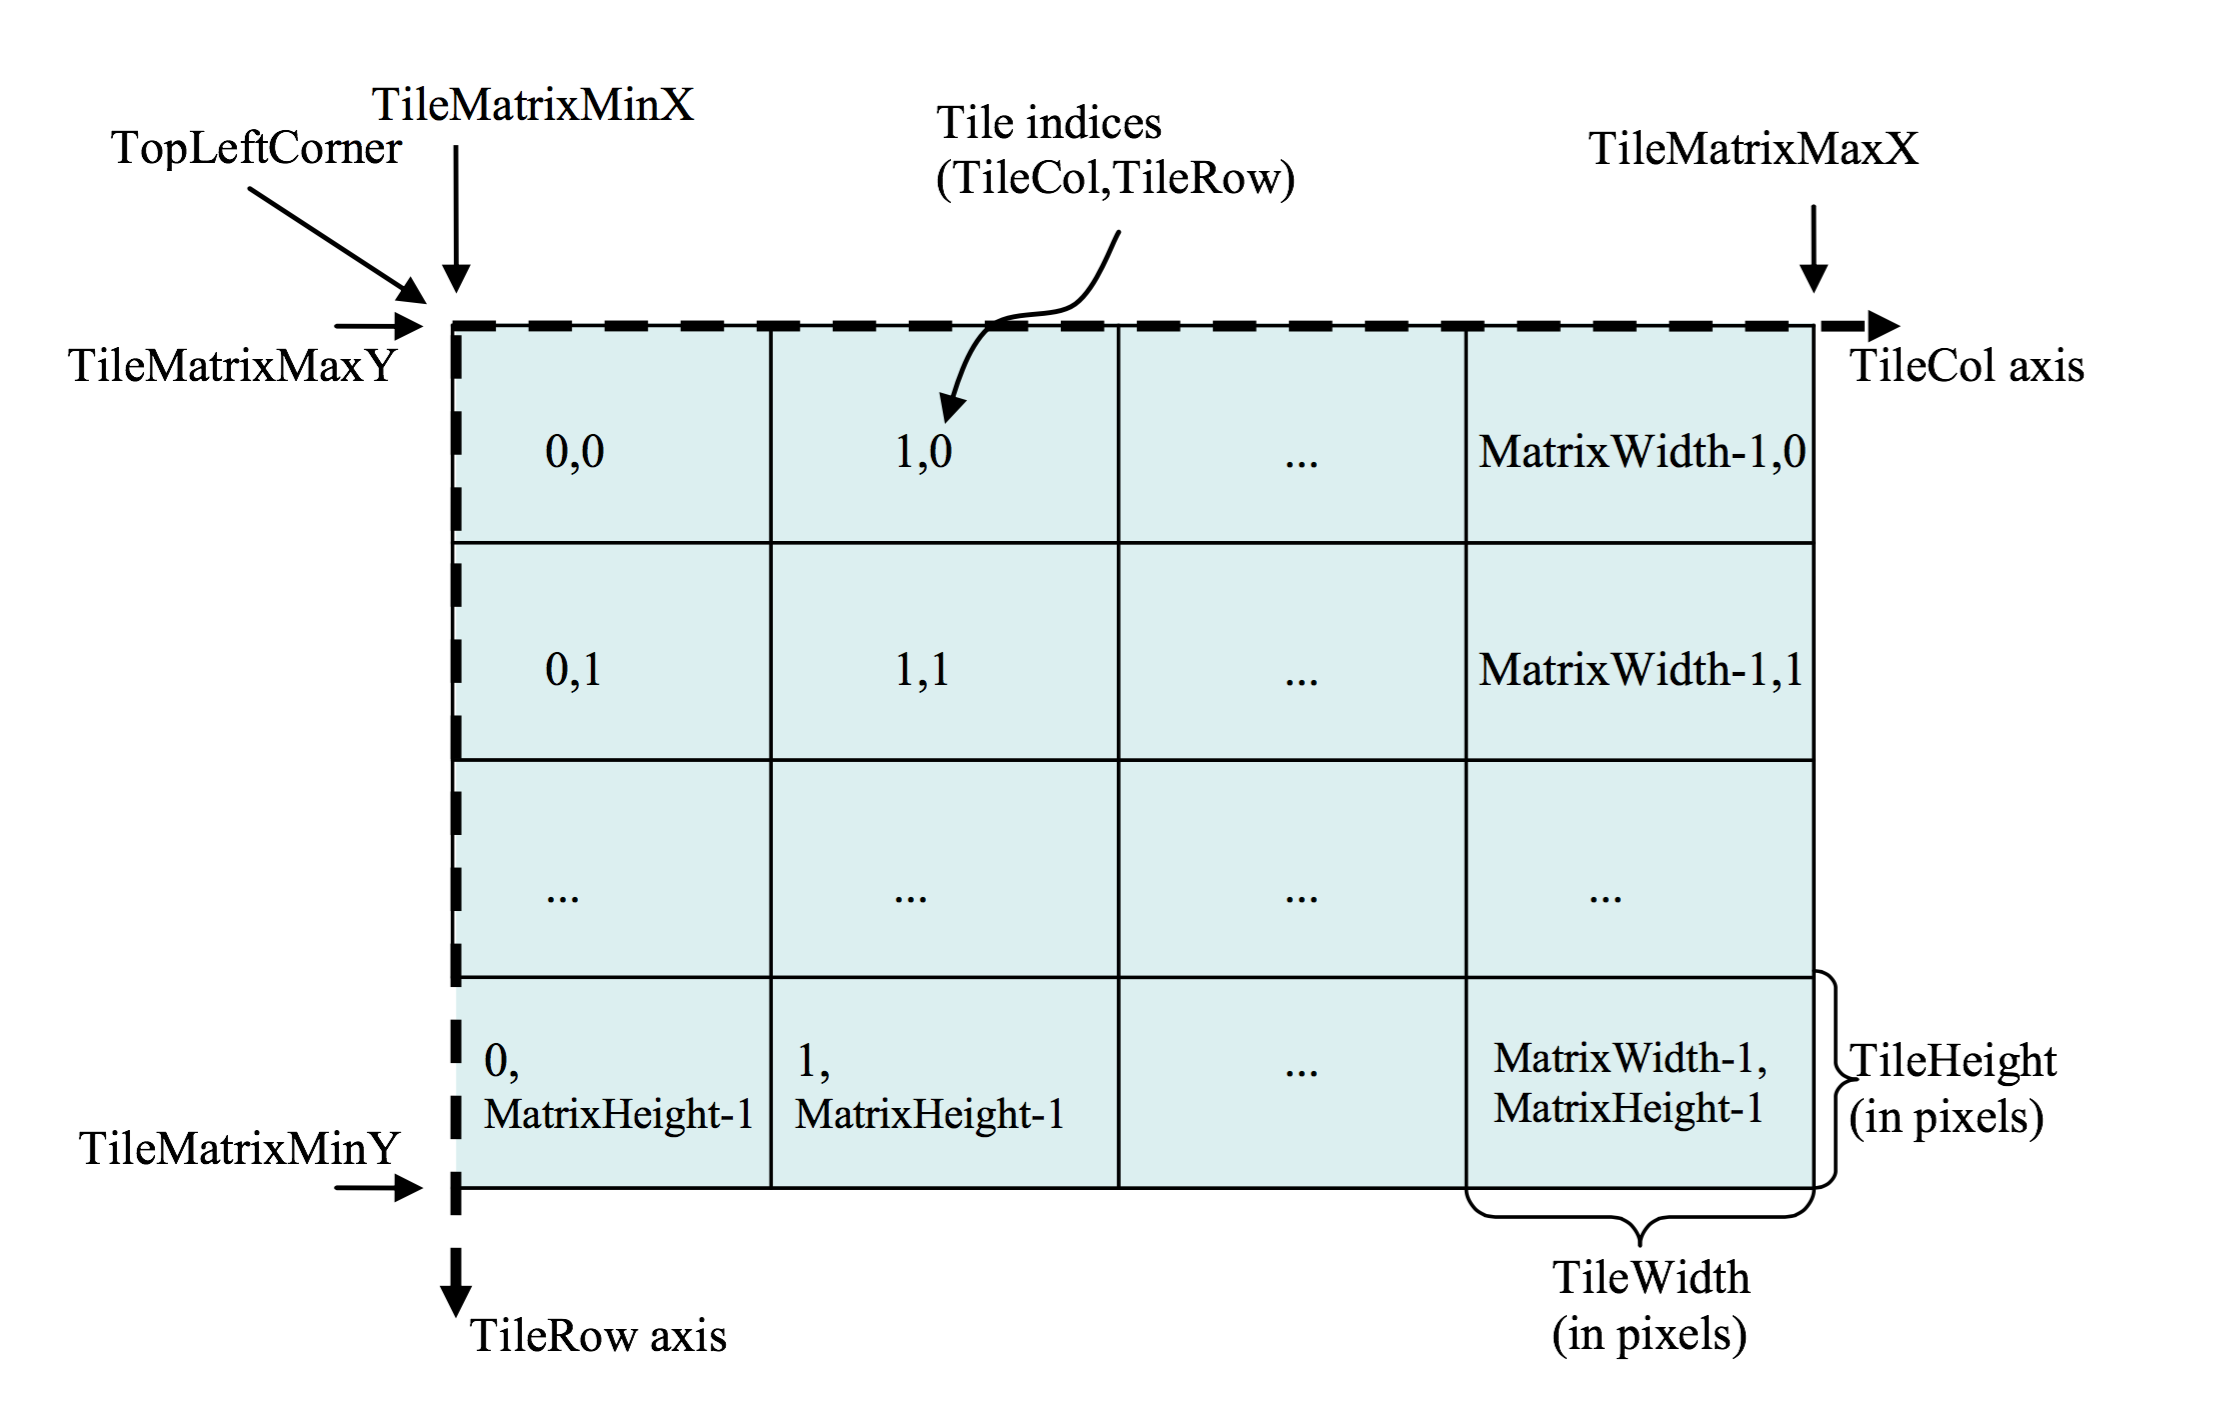
\includegraphics[width=\textwidth]{img/tile_matrix.png}
	\caption{Tile Matrix}
    \label{fig:tileMatrix}
  \end{subfigure}
  \begin{subfigure}[b]{0.5\textwidth}
    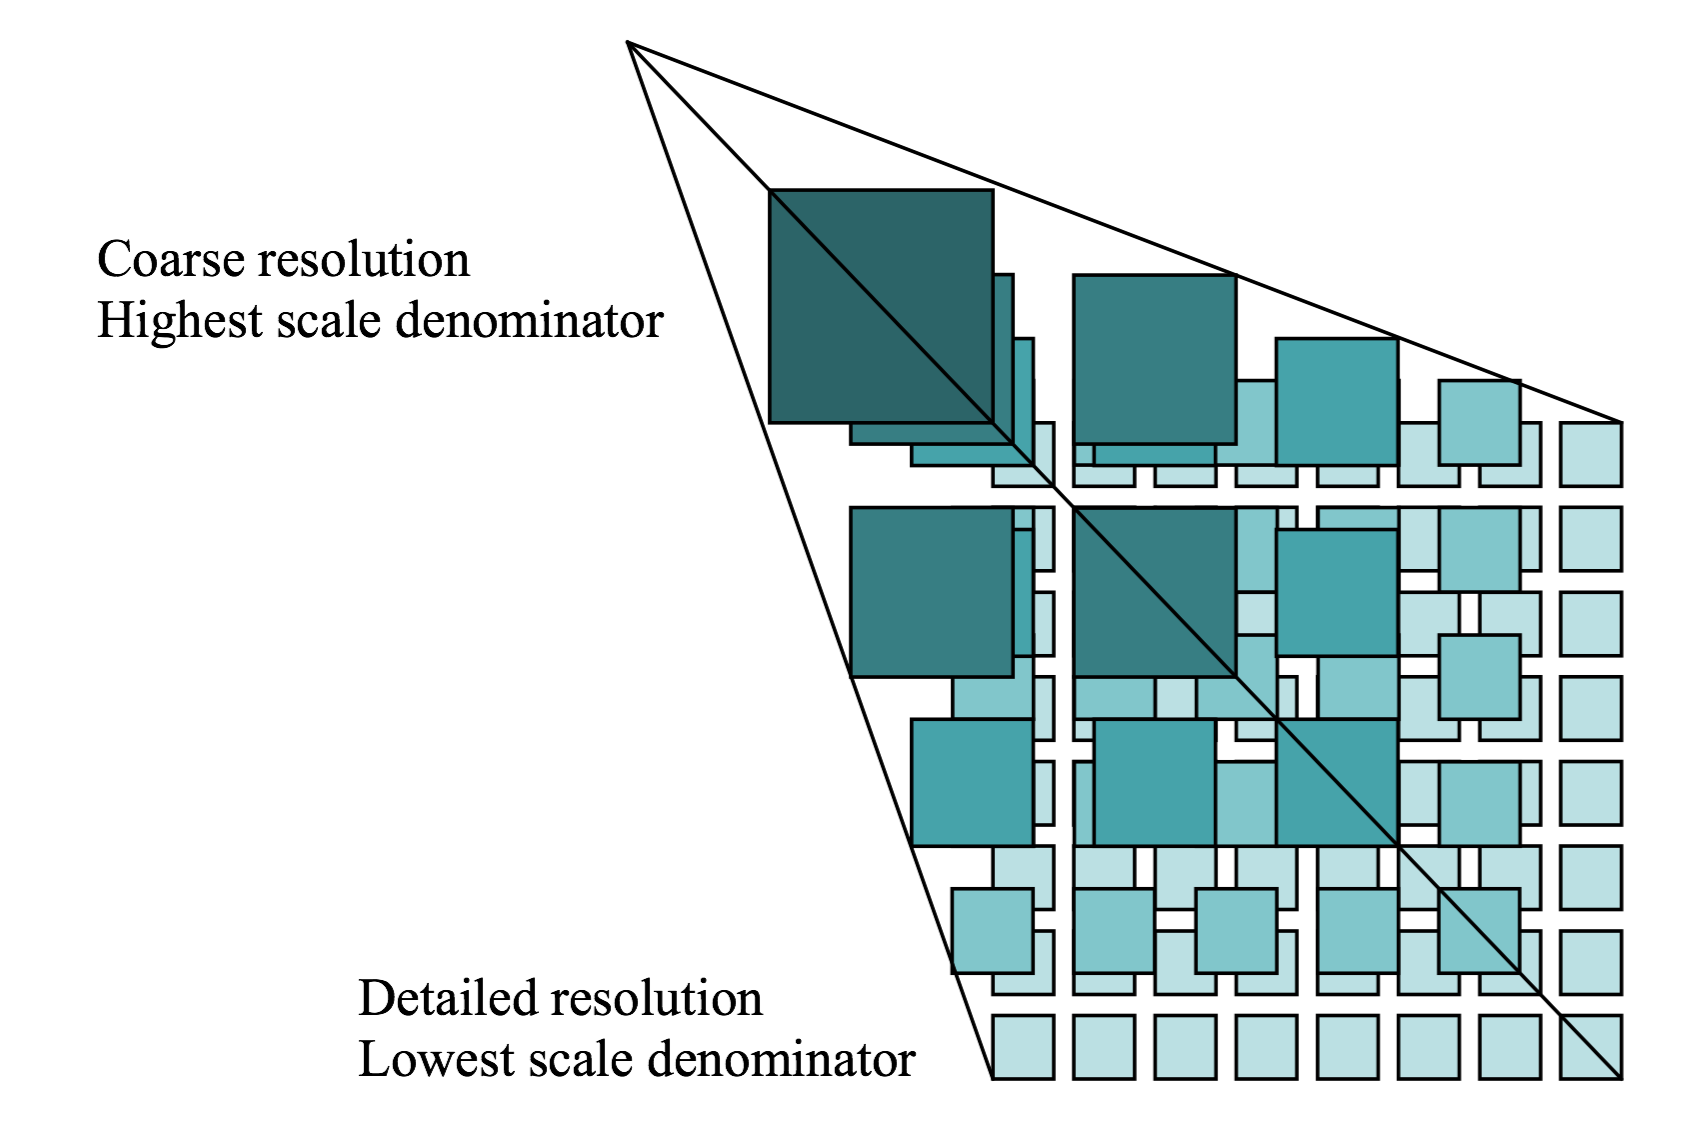
\includegraphics[width=\textwidth]{img/tile_matrix_set.png}
    \caption{Tile Matrix Set}
    \label{fig:tileMatrixSet}
  \end{subfigure}
  }
\caption{Tile matrixes}
\end{figure}

\section{Indexing}
\section{Projections}
\label{sec:ProjectionChallenges}
There is a fundamental problem with representing a curved surface such as the surface of the Earth, on a flat cartesian grid.
Since the Earth is a sphere, any map application will have to take this into consideration.  

In order to transform a curved surface into a flat surface, you need to do a mathematical projection of the curved surface onto a cartesian grid.
This process unavoidably results in a distorted result. Several different projections exsist, and some are more common or popular than others.
Some projections preserve the relative area of landmasses, while distorting shapes. Other projections preserves shapes, but distorts the relative size of areas. The distortion is more prominent at the extremes of the projected map.

\cite{mapProjections}.

\subsection{Different projections}
OpenLayers include two projection definitions, \textit{World Geodetic System} (EPSG:4326) and \textit{Web Mercator} (EPSG:3857). World Geodetic System is a standard used for cartography and navigation and Web Mercator has been popularized by web apps such as Google Maps. The problem with these projections is that landmasses near the poles appear much bigger than they in fact are.
This is the reason Sintef chose to use the \gls{PSP} which preserves angles, resulting in more acurate sizes of the landmasses and thus is more suited for navigation.
Because we had to display data from a source using \gls{PSP} on top of a background map using Web Mercator we had to reproject the data in order to make it fit on the map. This proved to be a non-trivial task. 


\begin{figure}[h]
\framebox[\textwidth]{
  \begin{subfigure}[b]{0.48\textwidth}
    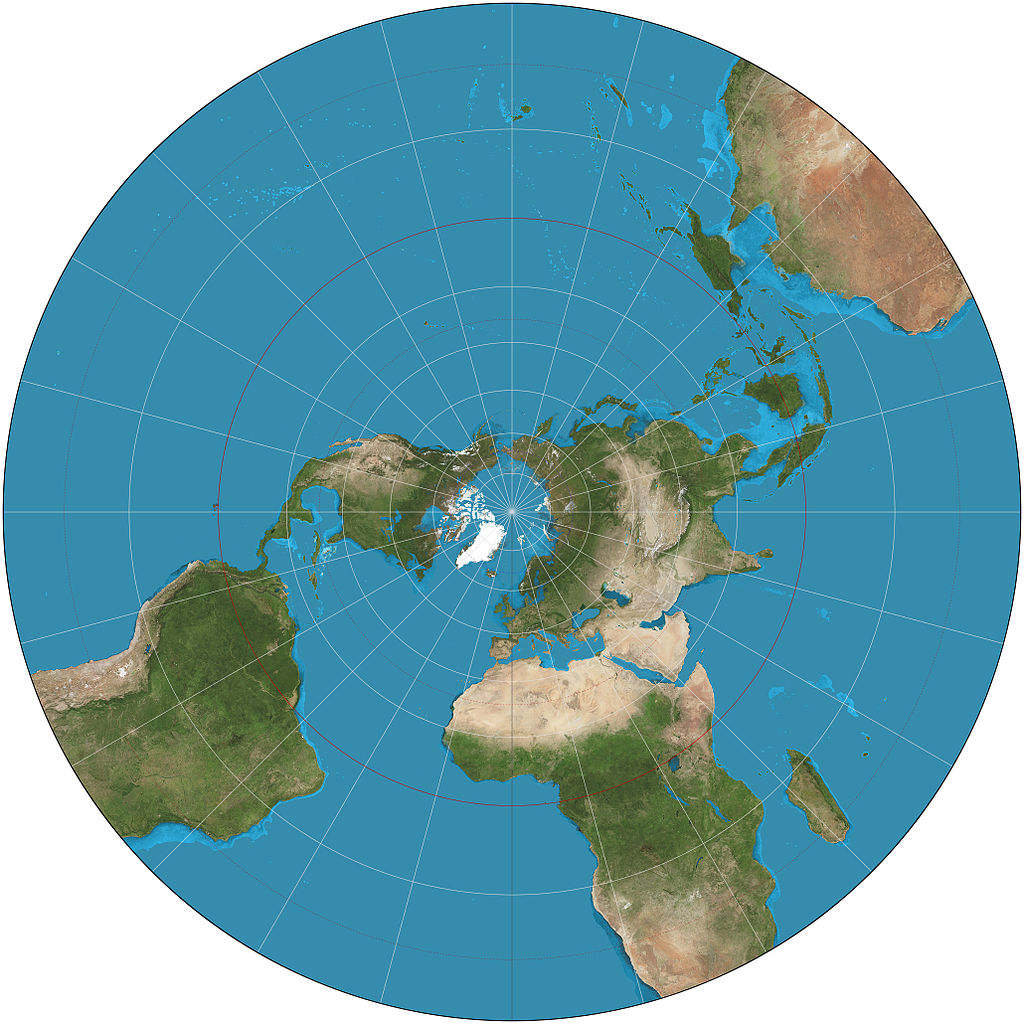
\includegraphics[width=\textwidth]{img/polar_stereographic_projection.jpg}
	\caption{Polar stereographic}
    \label{fig:PSP}
  \end{subfigure}
  \begin{subfigure}[b]{0.48\textwidth}
    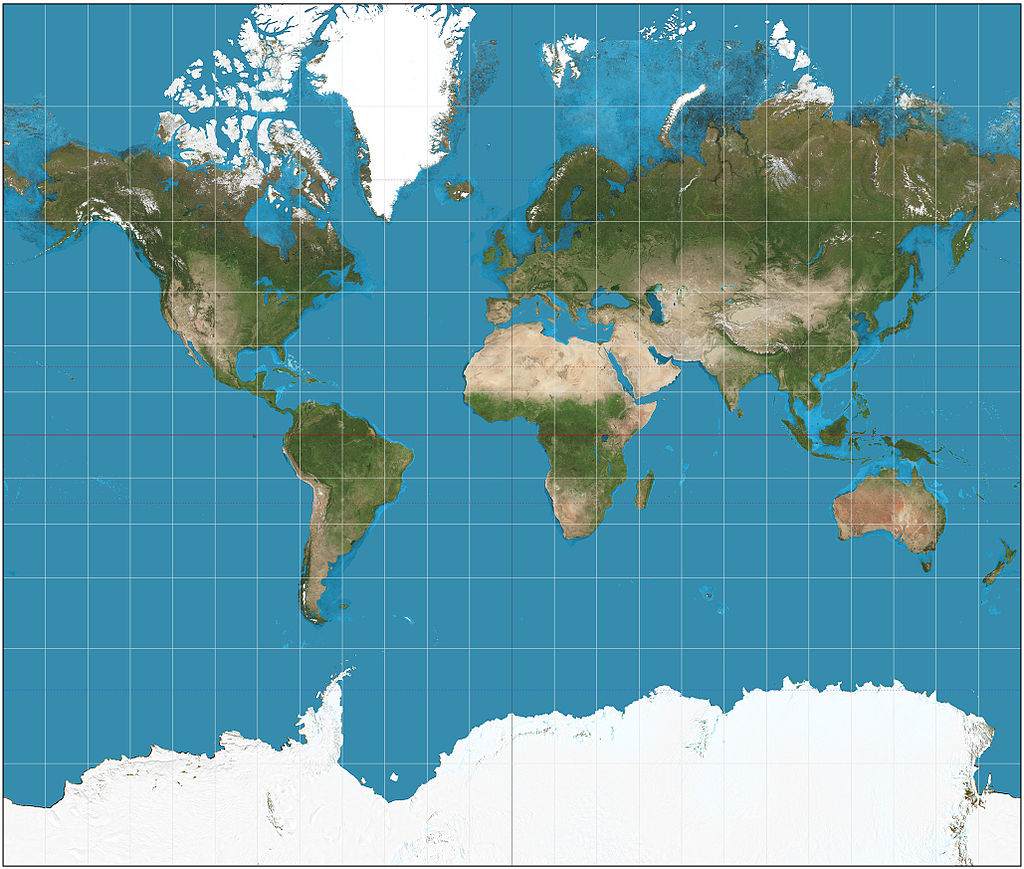
\includegraphics[width=\textwidth]{img/mercator_projection.jpg}
    \caption{Mercator Projection}
    \label{fig:mercator}
  \end{subfigure}
}
\caption{Different projections}
\end{figure}

\subsection{Attempted solutions}
\subsubsection{Dynamically projecting on the back end}
One solution we attempted was to dynamically project the dataset requested by the user. It was decided that this solution is too slow to be practical, as you have to pay the price of reprojecting the data every time it's requested. It also would have severely complicated the code: When reading a \gls{netcdf}, you can only read out a spatial rectangle that is aligned with the dataset.

When the user application requests a rectangle in a foreign projection (relative to the dataset), he is requesting what is effectively a trapezoid region of the data (in the native projection).
This means that we have to read out a rectangle that contains the requested trapezoid, do a costly reprojection computation, discard the superflous data points, resample the result and then return an image of it.

This is both impractical and expensive (slow), so we decided not to go down this path.

\begin{figure}[h]
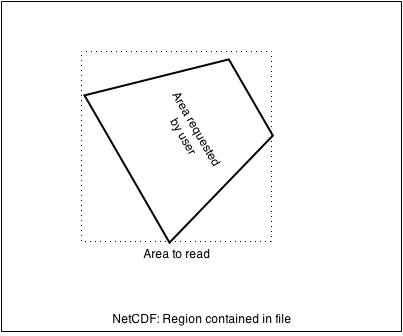
\includegraphics{img/dynamic_projection.png}
  \caption{Dynamic projection}
    \label{fig:tileMatrixSet}
\end{figure}


\subsection{Chosen solution}

\chapter{Final product}
\section{Description}
\section{Back-end}
\subsection{High level Architecture}
The \gls{back-end} is built as a single binary to ease deployment. The program consists of 6 major modules, each of which are described in more detail below:
\begin{itemize}
	\item Web server
	\item Rest endpoints
	\item \gls{netcdf} Manager
	\item Indexer
	\item Image renderer
	\item \gls{WMTS} module
\end{itemize}  

Using these modules, we have built two services: A \textit{REST \gls{API}} to query for arbitrary data, and a \textit{\gls{WMTS} service} to allow for easy creation of mapping applications.


\paragraph{REST API:}
The REST \gls{API} consists of a series of \gls{URL}s that can be queried to obtain slices of the dataset. The \gls{API} takes a set of data space constraints and returns an image representing the requested area at a given time and depth.

The control flow of the REST \gls{API} is as flollows:  
When a request comes in, it's automatically routed by the webserver module to the correct Resource class. The Resource class parses the parameters supplied by the user, and talks to the \textit{\gls{netcdf} manager} module in order to obtain the relevant data.
The manager module, in turn, can talk to the \textit{Indexer} to figure out which specific file contains the relevant data, before opening the given file and reading out the data. 
The data array is then passed back to the Resource class, which formats it according using the \textit{Image module}, and returns that as a response.

\paragraph{WMTS service:}
The \gls{WMTS} service follows the \gls{WMTS} \gls{protocol}\cite{WMTS:spec}.
This allows mapping application libraries to automatically lay out the data correctly on its map grid.  
Our \gls{WMTS} implementation reuses a lot of the capabilities and infrastructure built for the REST \gls{API}:  
For the capabilities document, we query the same Index used by \gls{netcdf} manager to get info about the extent (bounding box) of the dataset.
To get a specific tile, we compute the coordinates of the corners of the tile, and call the resource described above to retrieve an image.
We then put this image in a cache so that subsequent queries for this tile takes less time.

\paragraph{}
A more in-depth description of each module follows:

\subsection{Web server}
We use an embeddable web server library called Jetty\footnote{http://www.eclipse.org/jetty/} in combination with a REST library called Jersey\footnote{https://jersey.java.net/} to handle requests.
Jetty is being used in embedded mode, which means that the program contains a web server, instead of the other way around. This makes the code more portable, as it possible to change the web server implementation used without having to rewrite a lot of webserver-specific code.
Jersey is a REST framework for java. It adds a series of annotations and classes to simplify writing REST services.

\subsection{NetCDF Manager}
We have a module responsible for reading and parsing the data contained the dataset. When the other modules need to fetch any data from the dataset, they can call this module. This keeps \gls{netcdf} specific code in a single place and provides a single interface to query data.
This module uses a third-party library called NetCDF-Java\footnote{http://www.unidata.ucar.edu/software/thredds/current/netcdf-java/}

This module contains three main methods - \texttt{getScalarArea}, \texttt{getVectorArea} and \texttt{readDepthProfile}. Those methods are used for extracting different information from \gls{netcdf} files. Each of those methods accepts parameters to specify area, time and variable that should be returned. To abstract access to \gls{netcdf} variables, static enumeration with all features, that can appear in application, was created in \texttt{com.sintef.featureserver.netcdf.Feature}.

The workflow of every data providing method in \texttt{NetCdfManager} follows this scheme:
\begin{enumerate}
    \item Get all files that contain data that were requested
    \item Filter only relevant files (most recent and closest resolution)
    \item Read relevant data from files:
    \begin{enumerate}
        \item Open the file (\texttt{ucar.nc2.dt.grid.GridDataset.open(\textit{filename})})
        \item Get grid datatype (\texttt{findGridDatatype(\textit{netcdfVariable})})
        \item Get coordinate system (\texttt{getCoordinateSystem()})
        \item Get relevant subset of data (\texttt{makeSubset(...)})
        \item Count time and depth indexes
        \item Load data that were requested (\texttt{readDataSlice(\textit{time}, \textit{depth}, \textit{x}, \textit{y})})
    \end{enumerate}
    \item Copy data to output array and return
\end{enumerate}

Because of the time constraint, current implementation can read data only from one file, but the architecture is prepared for reading data from multiple files and joining it into one resulting array.

\subsection{Indexer}
The indexer scans the data folder for new \gls{netcdf} files, and keeps track of what kind of data is contained in each file. The \textit{\gls{netcdf} manager} module relies on this to select the correct file to open when asked to provide data.
\subsection{Image renderer}
The data is originally stored as an array of scalar values. The program has to render this array as an image in order to be useful to the user. This consists of taking a two-dimensional array, and turning it into an image.
The different resources rely on this module when the requested output representation is an image.

\subsection{REST endpoints}
The REST endpoints are gateway to the application as all communication flows through them and API is defined by those endpoints. It is a collection of classes representing specific service that the application provides. When user enters his request in form of \gls{URL} into his \gls{HTTP} client (browser), server parses this request and calls apropriate resource class to handle this request. The user can specify additional constraints in the form of query parameters.

In the application there are currently resource classes for checking status of the application and for representing scalar information from simulated dataset (current magnitude, depth, salinity and temperature). By specifying query parameters user can tell the endpoint which section of the data he is interested in. Most resources accept area, depth and time parameters.

Due to time constraints, we have restricted the output to require a 2D slice of area at a single time and a single depth. However, it should ideally be possible to query for any subspace of the dataset.

Every resource class has to be in the \texttt{com.sintef.featureserver.rs} class and is annotated by \texttt{@Path} annotation specifying the root \gls{URL} of that resource. Because most resources need to access information from \gls{netcdf}, it is common to store reference to \texttt{NetCdfManager} in a private variable in class constructor. Resource classes then contain methods for handling user requests. Such methods are annotated with \texttt{@Path}, which specifies path from the resource root and have to return \texttt{Response} object. Method parameters which are annotated by \texttt{@QueryParam} with parameter name are autofilled with query parameters.

Typical workflow of the class method for handling user request is to first validate the user input, then use \texttt{NetCdfManager} to get the data user requested, convert the raw data to some interchangeable format (usually to \gls{PNG} image with the use of \texttt{Image renderer}) and finally pack the result in the \texttt{Response} object and return it.

To minimalize boilerplate code, the \texttt{RsUtil} class containing common methods was created. This class contains methods for user input validation and for converting array of vectors to array of it's magnitudes.

\begin{minipage}{\linewidth}
\begin{lstlisting}[language=Java, caption=Example of a simple REST resource class, label=lst:resourceClass, frame=single]
@Path("root-of-my-resource")
public class MyResource {
    
    @Path("my-method")
    public Response myMethod(
        @QueryParam("myParam") final String param) {
        
        return Response.ok(param).type("text/plain").build();
    }
}
\end{lstlisting}
\end{minipage}

In the listing \ref{lst:resourceClass} is an example of a very simple resource class. This resource resides at \gls{URL} \path{/root-of-my-resource} and has only one method \texttt{my-method}, which accepts one parameter. After invoking this class by pointing your browser to \gls{URL} \path{/root-of-my-resource/my-method?myParam=test}, application should respond with "test" (which was our parameter) in body and the type set to text/plain.

\subsection{WMTS}

The \textit{\gls{WMTS}} module is tasked with generating a \textit{capbabilities document}, and serving \textit{tiles}. When generating the capabilities document, the \gls{WMTS} module calls the indexer in order to obtain the bounds of the entire dataset.

The \gls{WMTS} module also has to be able to take the tile index requested by the user and computing the coordinates of the corners of the given tile. If the image for this tile is already in cache, it can just return that to the user.
Otherwise, it then calls on the relevant resource with the computed coordinates to obtain the image for that tile. Finally, it calls the cache to store the image for later use.

Thus, the \gls{WMTS} module relies on the indexer, cache, and resource module. By proxy, it also relies on the data manager and image renderer as well.

\begin{figure}[!htb]
\begin{center}
\fbox{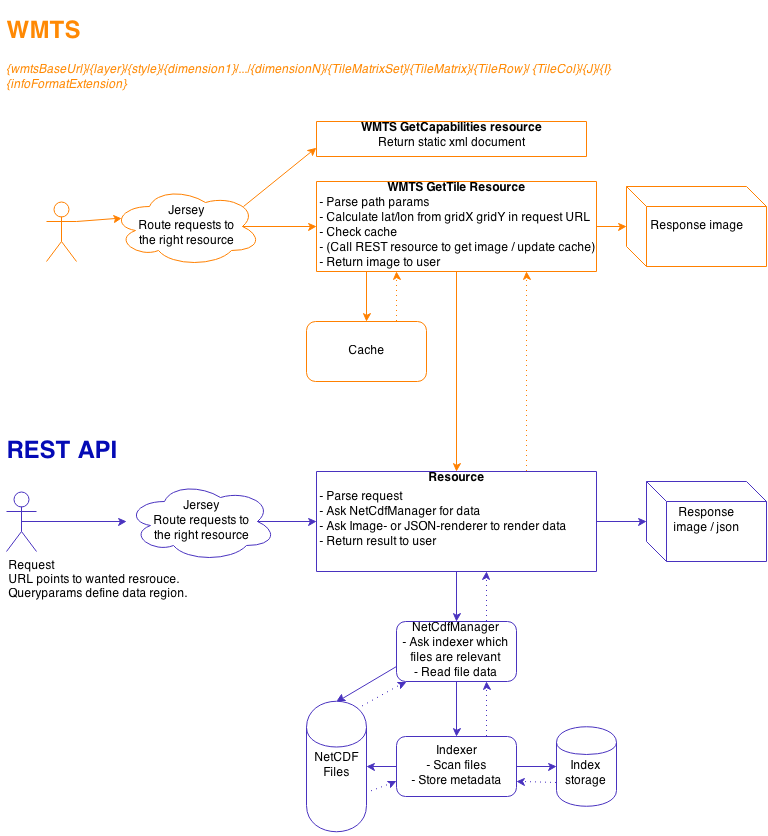
\includegraphics[width=400px]{img/back_end_arch.png}}
\caption{Back-end Architecture overview}
\label{fig:Back-endArchitecture}
\end{center}
\end{figure}


\subsection{Rendering data}
The ImageRenderer class is responsible for turning the raw data into \gls{PNG} images. An empty image is created and filled pixel by pixel from sampling the data. It can be used to create tiles for \gls{WMTS} or images that can be used outside a map service.
\paragraph{Inputs and Outputs}
The data it takes as input is in a 2 dimensional array of numeric values. In addition to the data, it takes parameters to tell it if the resulting image should be square, even if the input data is not. The last parameter contains what feature (e.g. salinity) is to be rendered. The finished image in the form of a BufferedImage Java object, ready to be transmitted as a response to an end users request.
\paragraph{Sampling}
The raw data is sampled simply using nearest interpolation. This is done in order to not misrepresent the accuracy of the underlying data. Bilinear interpolation may look smoother, but users would no longer see the grid that reveals the resolution of the underlying data.
\paragraph{Color}
Each feature has a hard coded scale, defined by a minimum and maximum value, and a color for each of these extremes. If the sampled value for a pixel lies between the minimum and maximum of that features scale, the color is assigned by linear interpolation between the minimum and maximum colors. If the value is outside the minimum to maximum range, that pixels color is set to the minimum or maximum color.
\paragraph{Size of the resulting image}
The image will be set to be 256 pixels along the shortest dimension of the raw data input, maintaining the aspect ratio as well as can be done. If the function is told to make a square image, by the forceSquare parameter, the result will be a 256 by 256 pixel image.

\section{Front-end}
The \gls{front-end} consists of a single \gls{HTML} file, the OpenLayers javascript library, custom javascript and \gls{CSS}. These components combined make up the \gls{GUI}. Its role in the product is to help the user querying the \gls{back-end} and then displaying the received data in a meaningful way. 

\paragraph{Graphical User Interface}
The main job of a \gls{GUI} is to make the user able to interact with the application. In the case of our product the main features are querying and displaying the received data, primarily on a map. Because the map has such an important function in the application we chose to make it as big as possible. This emphasizes the importance of the functions related to the map and makes it easier to veiw the data displayed on the map. The map is provided by the OpenLayers javascript library which gives the possibility to display maps and data from different source. Since we want to display data that is closely related to geographical position, displaying it on a map is the most intuitive solution. In order to make it as easy as possible to query the \gls{back-end} for data we have added a input box. The user can toggle this input box to be hidden or not. Being able to hide the input box helps to keep the screen uncluttered and makes it easier for the user to focus on the displayed data.

\begin{figure}[!htb]
\begin{center}
\fbox{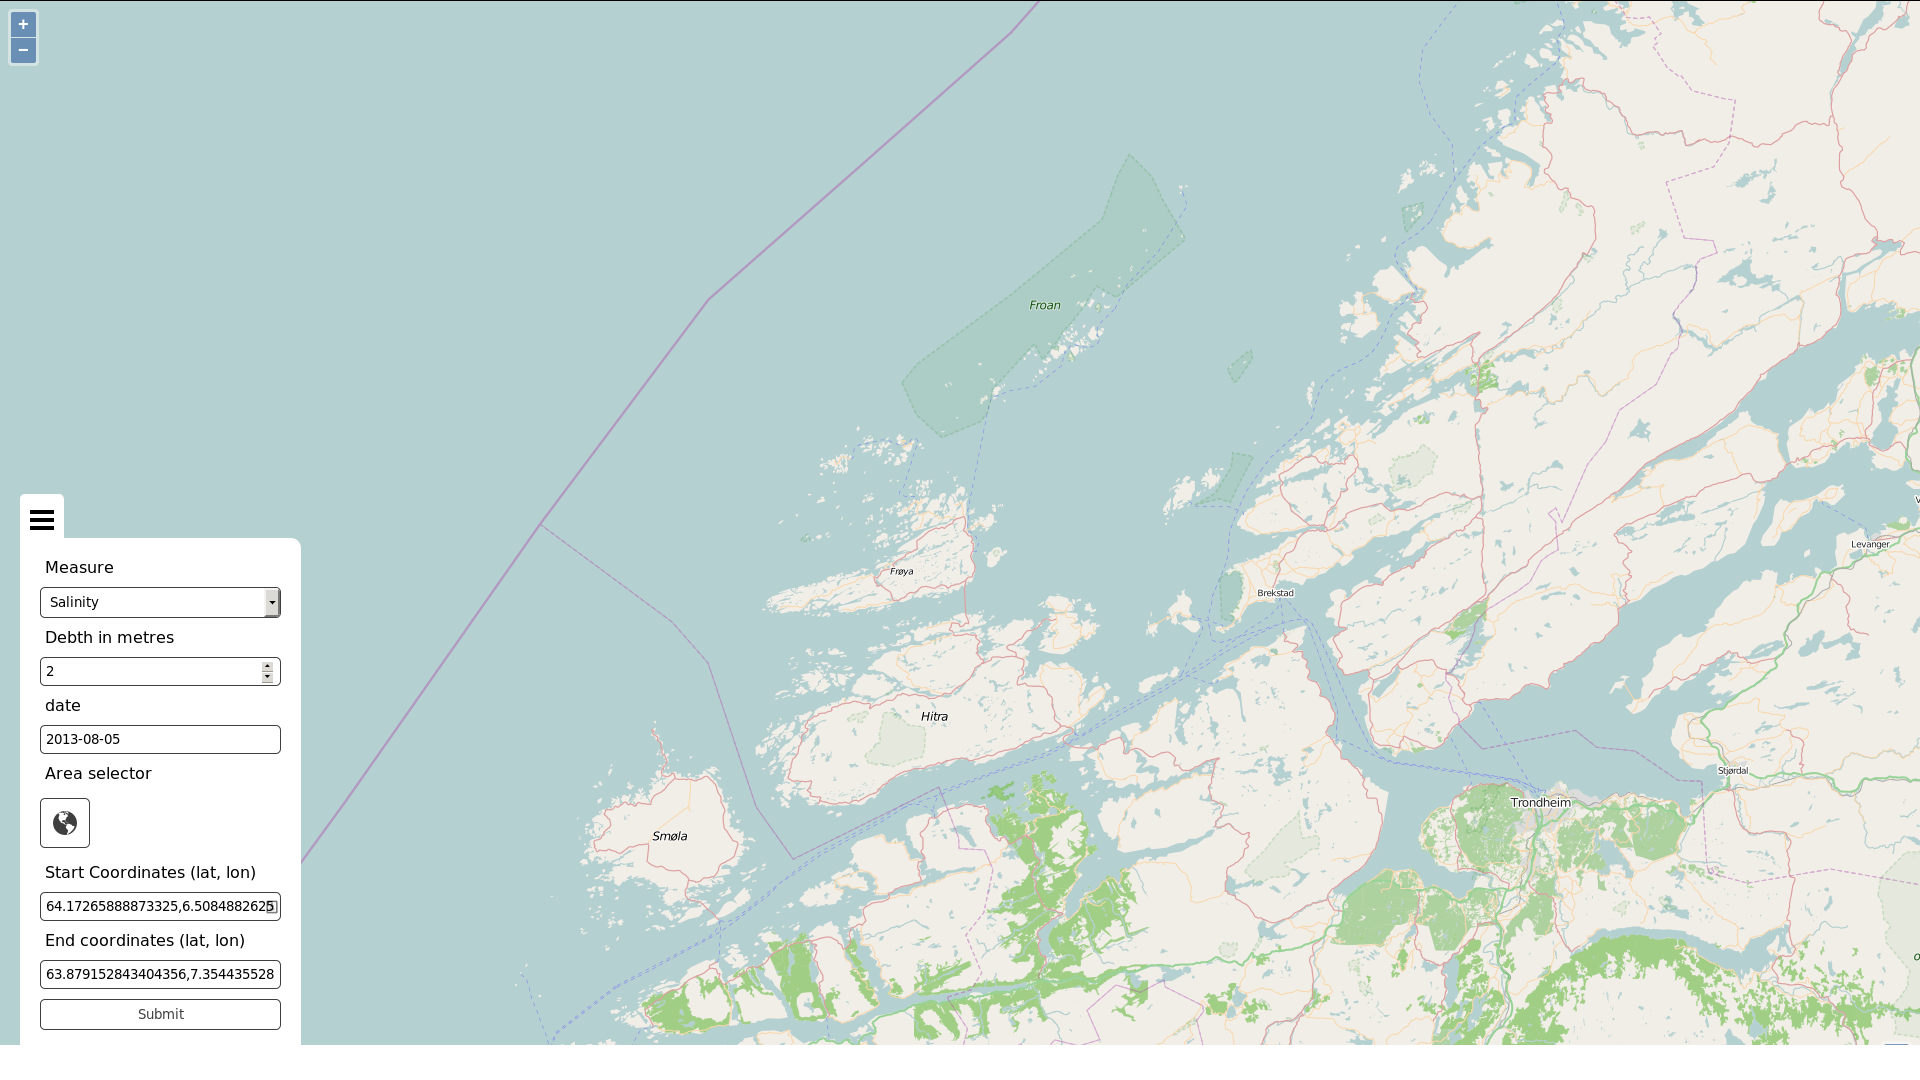
\includegraphics[width=400px]{img/gui.png}}
\caption{The graphical user interface}
\label{fig:gui}
\end{center}
\end{figure}

\paragraph{Querying}
Querying the \gls{back-end} is done by means of it's REST \gls{API}. This is done by taking the validated user input and building a query \gls{URL} from it. When the \gls{back-end} receives the input it processes it and responds with the relevant data, usually an image. The data response is then displayed in the \gls{GUI}, usually on the map at the user-defined coordinates. 


\section{Goal completion}
\section{Further work}
Given the size and complexity of the project, the functionality of the implementation had to be limited to the bare minimum. That means that further work should be done to meet the functional requirements for a commercial product. Many of these functionalities have however been considered during the project and therefor we have made some evalutations on how this can be done. In this section we present our suggestions for what can be done to improve the implementation.

\subsection{Front-end}
For the front-end there are new kinds of data that should be displayed in the GUI, some of which lack implemented back-end support. First off the basic map overlay requires some improvements. This includes extending the functionality it provides and improving efficiency and scalability. Secondarily there are new functions to be added, ranging from new controls to displaying other types of data.
\paragraph{WMTS todo}
%WMTS? \ get map fully up and running

\paragraph{Point values}
%TODO
%describe pop-ups here
%follows up in Charts

\paragraph{Charts}
In addition to the point values the front-end should be able to display current roses, depth-cuts(?) and other calculated charts for a selected point. These charts would be served from the back-end, and will require a new brand new set of implementations. The back-end will then provide images to represent the charts. The task of the front-end is to find out how to display these images in a useful and intuitive way. 
\begin{figure}[!htb]
  \begin{center}
    \fbox{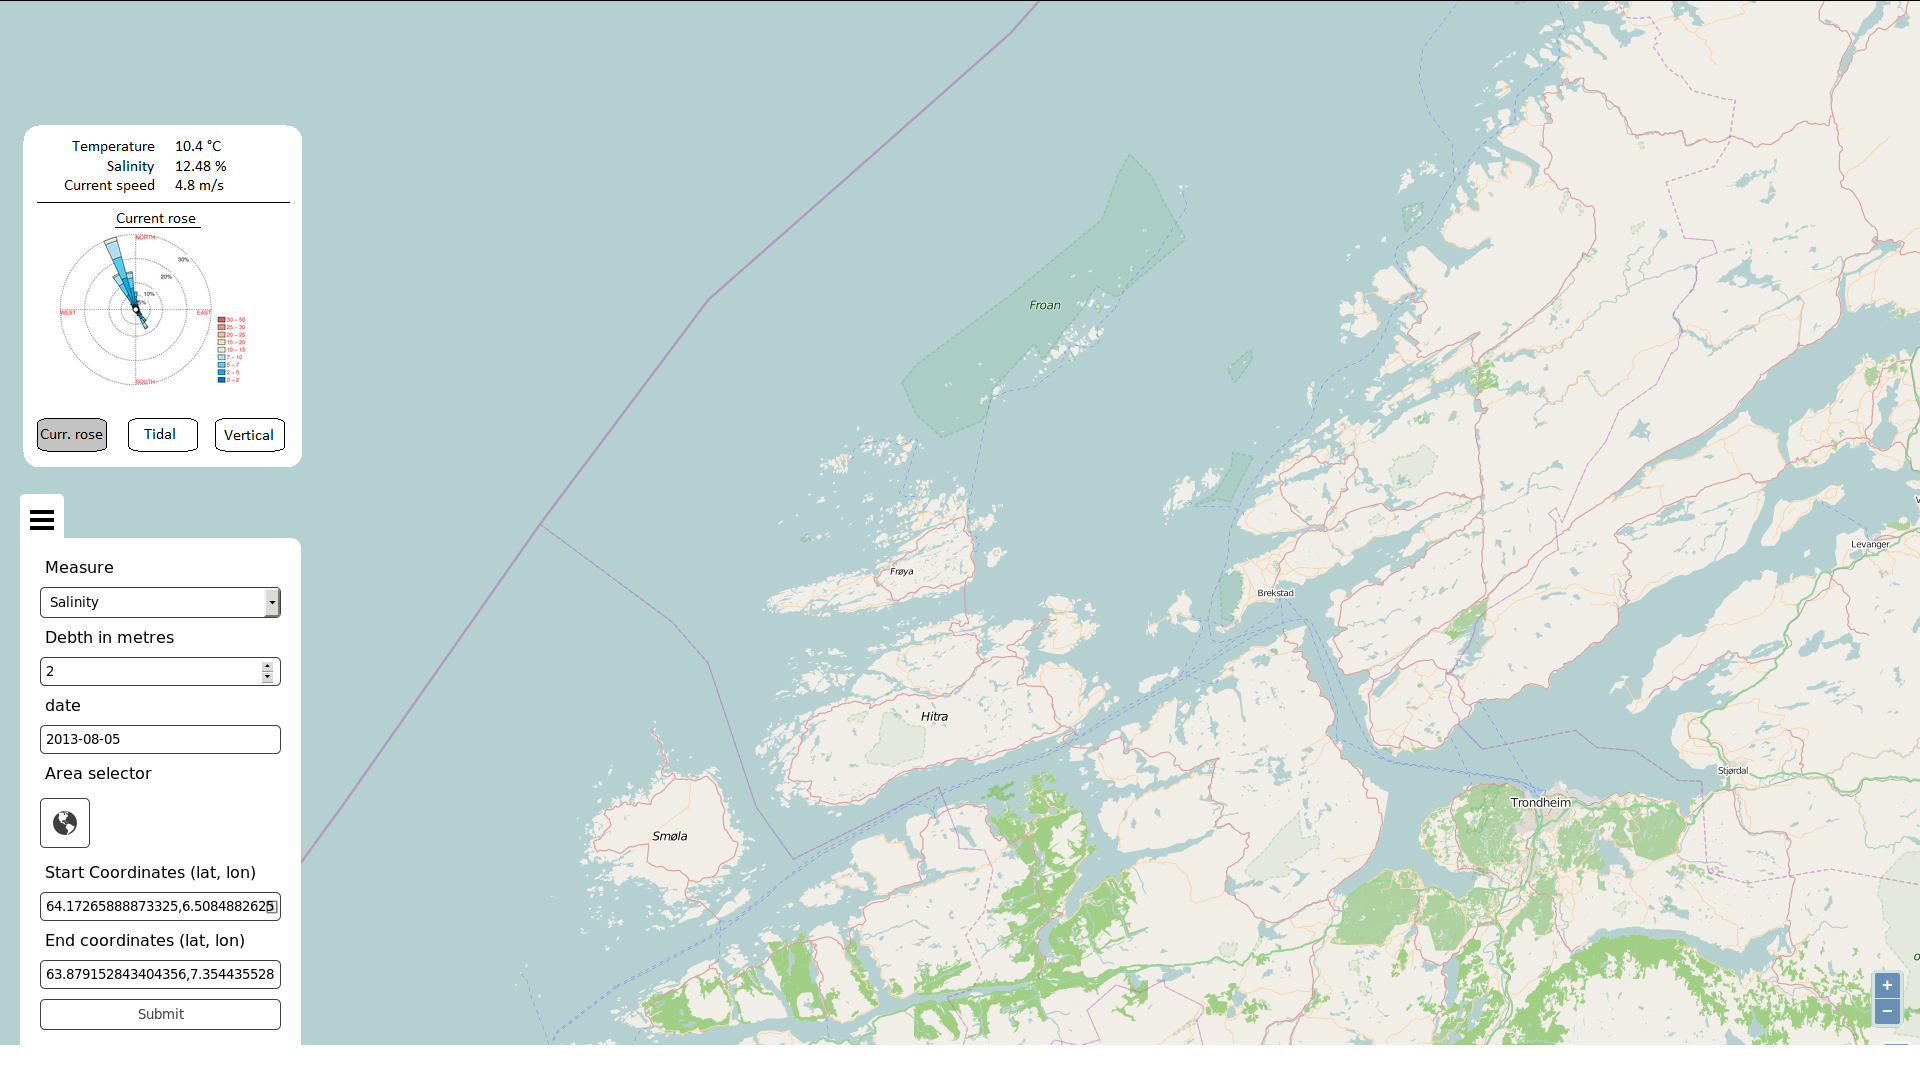
\includegraphics[width=\textwidth]{img/gui_charts_basic.png}}
    \caption{Example of how the basic charts can be displayed in the GUI}
    \label{fig:gui_chart}
  \end{center}
\end{figure}

\begin{figure}[!htb]
  \begin{center}
    \fbox{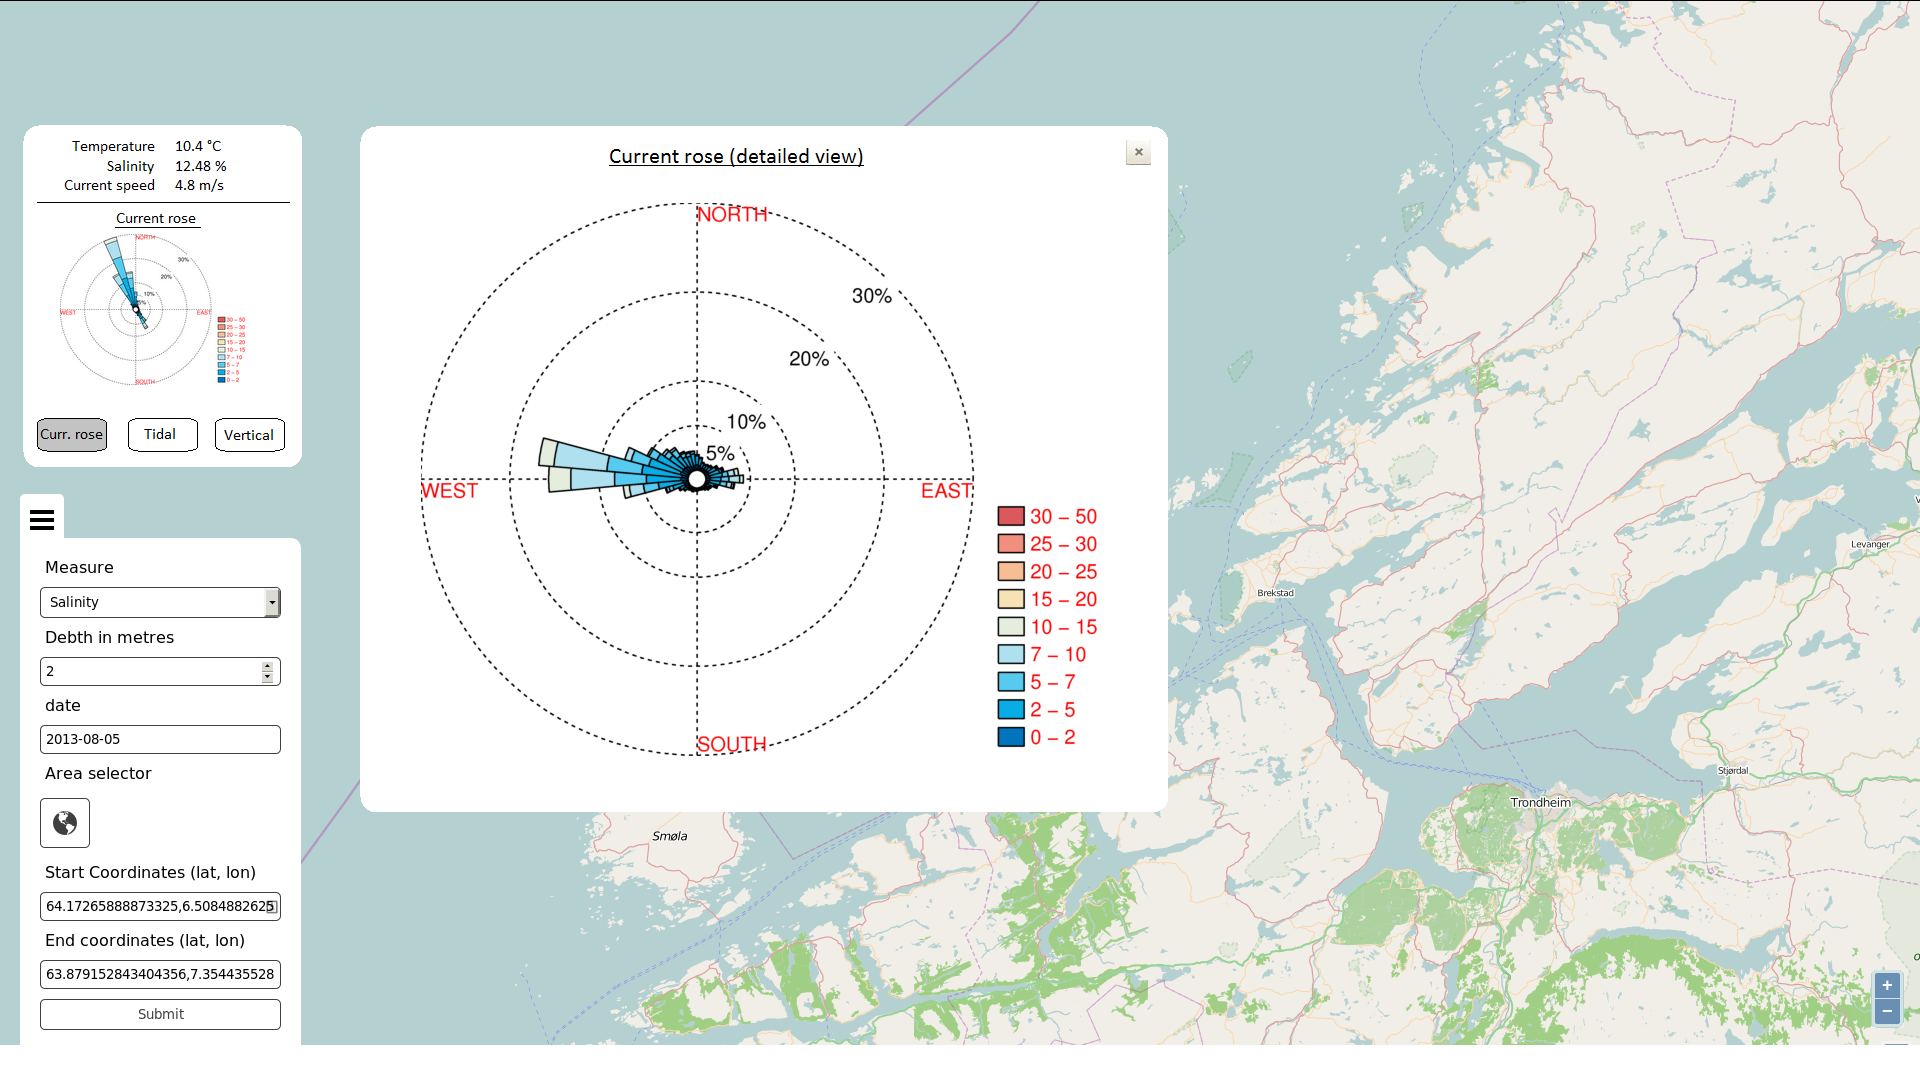
\includegraphics[width=\textwidth]{img/gui_charts_enlarged.png}}
    \caption{Example of how the charts can be enlarged}
    \label{fig:gui_chart}
  \end{center}
\end{figure}

% \begin{figure}[h]
% \framebox[\textwidth]{
%   \begin{subfigure}[b]{0.48\textwidth}
%     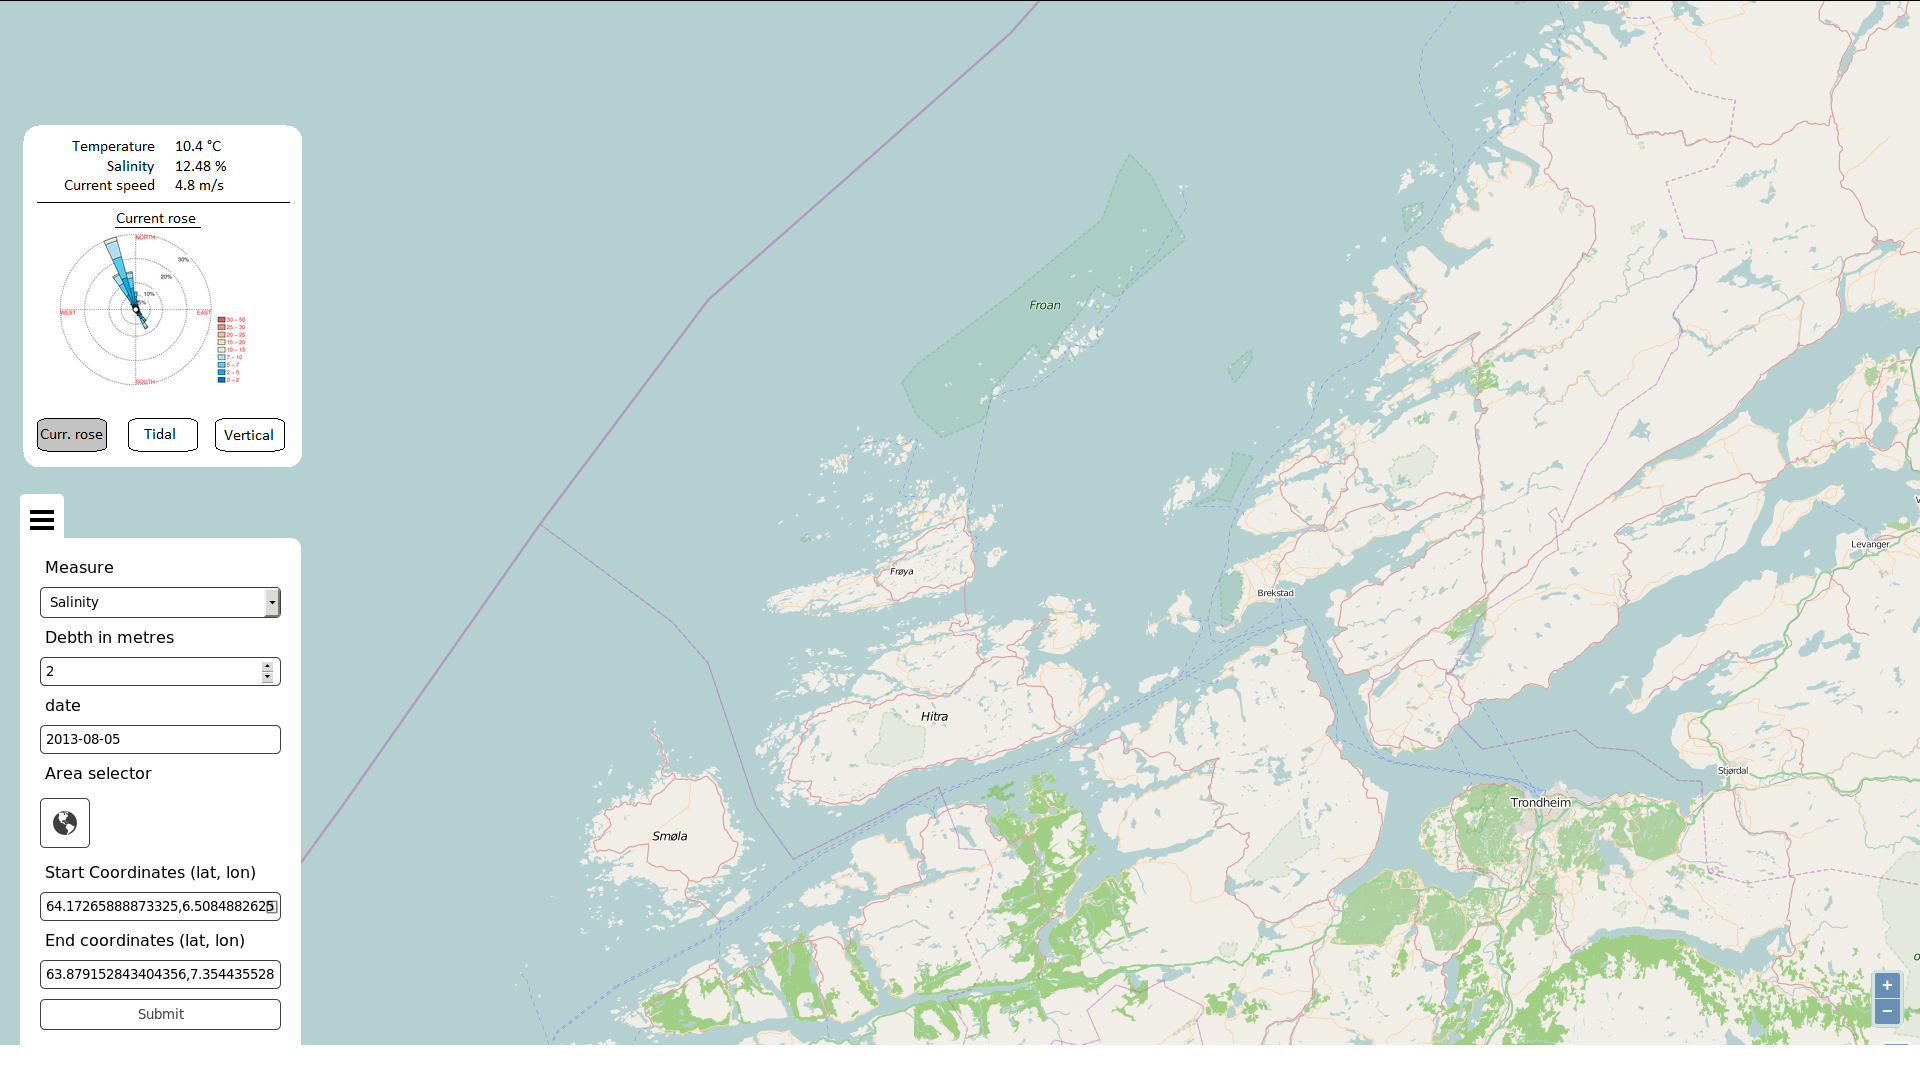
\includegraphics[width=\textwidth]{img/gui_charts_basic.png}
%   \caption{Charts}
%     \label{fig:PSP}
%   \end{subfigure}
%   \begin{subfigure}[b]{0.48\textwidth}
%     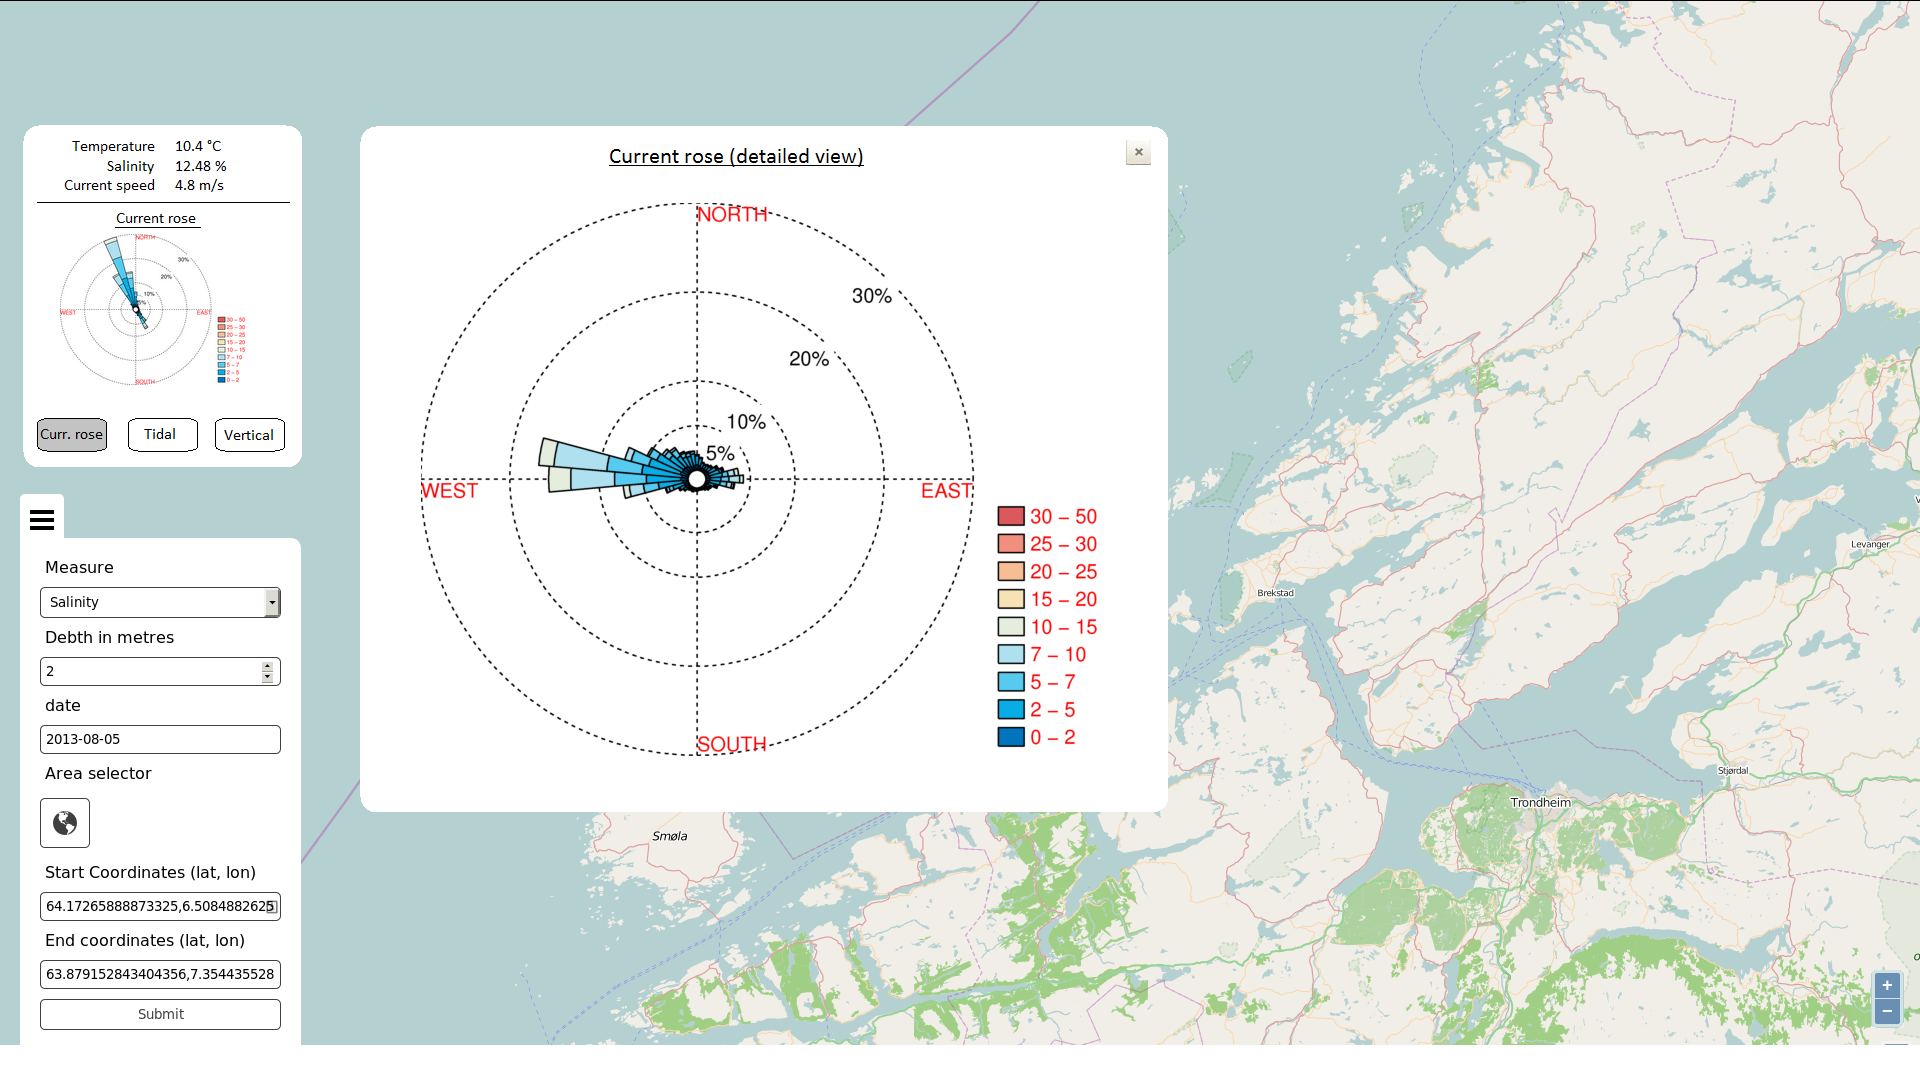
\includegraphics[width=\textwidth]{img/gui_charts_enlarged.png}
%     \caption{Charts enlarged}
%     \label{fig:mercator}
%   \end{subfigure}
% }
% \caption{Different projections}
% \end{figure}

\paragraph{Vector data}

\paragraph{Legend}

\paragraph{Seasonal averages} %Also point for back-end further?

\paragraph{Authentication}

\paragraph{Responsive design}
Website are increasingly beeing accessed from smart phones and tablets. But websites that are designed to beeing displayed on a desktop or laptop screen are often not well suited for mobiles and tablets. One solution to this is to have a dedicated mobile website. This solution comes with the drawback of having to maintain two sites. A solution that has gained traction and is the most common way by now is using so called responsive design. This means that the website changes layout depending on the resolution of the device the website is accessed from. This is achieved with \gls{CSS} media queries.
We knew from the begining of the project that accessing the application from smart phones was desireable. Therefor it should include responsive design. The layout as of today is quite simple and it would be relativly easy to write the needed media queries to make it responsive. In the form the application has at the time of writing it would not make sense to use a framework like Bootstrap \footnote{\url{http://getbootstrap.com/}} to gain responsiveness as it would introduce a lot of code to the project that would not be used. 

\paragraph{Icons}
The icons used in the GUI are called Octicons\footnote{\url{octicons.github.com/}} and are created by Github\footnote{\url{www.github.com}}. The font itself is licensed under the SIL OFL and the acompanying code is licensed under the MIT license \footnote{\url{www.github.com/github/octicons/blob/master/LICENSE.txt}}. This allows the icons to be used in commercial use. That said the icon font is not the most extensive one. If the applications grows and evolves it might be benificial to use a custom icon set or aquire one that has more relevant icons.

\paragraph{Minification}
When deploying a javascript application it is common to minify the code. This means that you use a tool to remove all white space, new line characters and comments from the code. The tool may also rename variables in the code. The purpose on this is to make the file as small as possible. Having a small script file matters because the file is downloaded to the client and thus has an impact on response time of the application. We have not used an minifier. As the \gls{front-end} code base is relativly small little is gained from minifying but as the code base grows in the future this is strongly recomended.

\paragraph{Tool tips}
A tool to select the area you want to query was added. It's toggled on and off by pressing a button in the \gls{GUI} or you can hold down the shift button on your keyboard while clicking and draging on the map. The keyboard shortcut is not mentioned anywhere in the \gls{GUI} and the user will propably not find this feature on his own. We therefor recomend that tool tips and hint are added to the \gls{GUI} so the user knows about all og it's features.

%OTHER?

\subsection{Back-end}

\chapter{Evaluation}
In this chapter, the group will give a thorough evaluation of the project, in respect to the groups own work and teamwork, the decisions made early in the project, time used, the subject and its organization, relations with the customer, and reflect on the team. 

This chapter will give a sense of what the group has learned through the project, what they want to repeat in future projects, and what could be improved. As well as determining these factors, we want to investigate what the causes of problems the group has experienced might have been, and attempt to suggest what could have been done to mitigate this. 

This chapter also serves as the groups reflection note, as the groups have been asked to include them in their report. 

\section{Product evaluation}
At the end of the project, the team has produced a \gls{prototype} \gls{front-end} and \gls{back-end} that demonstrates that it is feasible to replace the current system used by SINTEF to serve current data, with a new and customary built system. Finding out whether or not this is feasible has been the main task of the team, and we feel that has been completed successfully. 

\paragraph{Front-end}
The front end of the system shows a map of the world, and the user can either enter coordinates manually or by using a tool to graphically select the area they want. When the data is returned, a legend is displayed to explain the color gradients in the returned image. It is also possible to click a certain point of the returned data to get detailed information for this point.

The team is happy with the developed features for the \gls{front-end}. They have been well discussed with the customer, and developed in accordance to the customers wishes. To be able to implement more \gls{front-end} features, the team would have needed more time developing the \gls{back-end} to serve the correct data. 

\paragraph{Back-end}
The \gls{back-end} of the system is able to read from a \gls{netcdf}-file, and serve an image illustrating the data to the \gls{front-end}. The major challenges, as described in chapter \ref{chap:Challenges}, has been to index the files correctly, and to transform the data into the correct projections. 

The work on indexing came a long way, and was stopped just shy of actual testing, as the projections needed to be correct to be able to determine if the system worked correctly. The team is however confident that the work done on indexing is close to solving the problem.

Projections have been the major showstopper for the project. All parts of the solution relies on the projections being correct, and so, there was no real value in starting making functionality for graphs and other data, before this problem was solved. 

\paragraph{Summary} While the team was able to demonstrate to the customer that such a system can be implemented, and has implemented both a front- and back-end \gls{prototype}, the group had hoped to be able to finish more features. The fact that this has not been done is in large down to the challenges faced by the team, and described in chapter \ref{chap:Challenges}. Had the team been able to solve these challenges earlier, or had more time, several more features could have been implemented.

Though the team would have liked to have gotten further on the implementation, the customer has expressed that the work done on solving the different challenges faced by the team, is valuable to them. It will make future work easier, and a lot of the ground work has already been done. As such, the project has provided value to the customer, which is the most important part of the project.

\newpage
\section{Work evaluation}
In this section, we will look at the work the group has done, and how the different parts of the work turned out to be positive or negative for the project as a whole. In section \ref{subsec:Teamwork} we will discuss the work and relationship in the team. In section \ref{subsec:ToolsEvaluation} we will look into the different tools the group decided on using at the beginning of the project. We will then have a look at the time use in section \ref{subsec:TimeUsed}, before looking at the adaptations done to the scrum methodology in section \ref{subsec:ScrumAdaptationsEval}. We will then look at the customer relations in section \ref{subsec:CustomerRelations}.

\subsection{Teamwork}
\label{subsec:Teamwork}
In this section we will evaluate the work of the team. We will look at the cooperation, communication, punctuality, advisor contact and social interactions of the team. These are all important factors, that together form the foundation of the work the team will do.

\paragraph{Cooperation}
The group has had a good cooperation throughout the project. There have been no personal conflicts, while there has been room to disagree on an academical level. In the start of the project, the team agreed that disagreement is a good thing, as they are purely professional. Sticking to this principal has been key to maintaining a team environment where ideas can be discussed freely. 

The team has met 2-3 times a week, depending on whether a customer meeting was scheduled or not. During these meetings there as been room for group members to bring up issues they have, and it has been an arena where the group has been able to talk about their work and progress in general. 

During the implementation phase of the project, the team has divided into to sections. One section has been working on the \gls{front-end} of the project, and one on the \gls{back-end}. This has been a good way to divide work and responsibility. The cooperation between these to sections has been good, and changes that have affected the other sections work has been communicated. 

\paragraph{Communication}
The group has had two main communication channels: team meetings and Slack. Team meetings have been used to catch up on the status of everyones work, discuss what direction to move in, and distribute tasks between members. As far as possible, the team has attempted to have all conversations that needed some form of plenary discussion in meetings where everyone could be present.

All other communication has mainly been done using Slack (see section \ref{subsec:Slack}). This way, all communication has been available to every team member. It has been possible to ask a question to everyone, and start a discussion, without having to gather the entire team in one physical location.

The communication in the team has worked well in this project. Team members have known what is to be done, where to meet for meetings, and how the project has been progressing. Through several meetings every week, and the use of Slack, information has flown to all members of the group.

\paragraph{Punctuality}
At the beginning of the course, the team agreed that it would be important for everyone to be on time for all meetings. Meetings that start late are an annoyance to everyone who was there on time, and they also waste time that could have been better spent. It was decided that no sanctions should be necessary.

Throughout the project it has been an issue that team members have been late for meetings. This is most critical when meeting the customer and advisor. Unfortunately, these meetings have on average been 5 minutes delayed due to late team members. To compensate for this, meetings have been started even though not all team members have been present. This seems to have been an incentive for team members to be on time, as this has been a smaller problem towards the end of the project. 

\paragraph{Advisor contact}
Throughout the project, the group has had meetings with their advisor every week. The exception has been one week in september and the last week of the project, as the advisor was away. The goal has been that all team members should be present at this meeting every week. On average, 6 of 7 members have been present at the meetings.

The advisor meetings have been very valuable to the team. They have created an arena for the team to talk about the progress of the group as a whole, the different challenges faced by the team, and to get an external perspective on the work that has been done. 

With this in mind, the advisor meetings has in many ways served as the retrospect in scrum (see section \ref{subsec:scrumadaptations}). They have not been structured as such, but they have enabled the team to identify work techniques that have been successful, and not successful. 

\paragraph{Social interaction}
When working in a team, knowing each other on a more personal level can help teamwork. Meetings are smoother when team members know more about each other, members are more likely to honor their work quota if they face disappointing their friends, rather than strangers. It is easier to ask someone you know to do their share of the work. Knowing the other team members better will also give an incentive to spend more time with the team, and thus doing more work, and getting to know each other even better.

As most team members did not know each other very well at the beginning of the project, the possibility of setting aside some time to get to know each other was discussed. The team agreed that this was something they wanted to do, but failed to find time for this. In retrospect, the team should have prioritized this. The teamwork has, as described earlier, not been as good as it could have been. Some of this can be tracked back to the fact that the team members do not know each other very well.

\subsection{Tools evaluation}
\label{subsec:ToolsEvaluation}
In chapter \ref{chap:ToolsAndTech} we looked at the different tools and technologies the group has decided to to use for the project. Here, we will evaluate the use of the tools, and attempt to conclude on whether the decision to use the tool was productive for the project.

\paragraph{\LaTeX}
Using \LaTeX{} has posed some challenges for the team, but all in all, it has proven to be a great tool. \LaTeX{} allows for the writing of large and complex documents, but makes the writer focus on content, not presentation. This has been great for us, as the report is a massive document with images, tables, graphs and cross referencing. While using these advanced features of \LaTeX{} was difficult in the beginning, the team has saved a lot of time that would have been used going trough the document, checking to see if the formatting done had been broken. 

Some challenges the team has run into have been:
\begin{itemize}
\item References not compiling correctly due to different citation styles
\item Correct placement of images
\item Correct placement and formatting of tables
\item Making LaTeX accept special non-English characters
\end{itemize}

Most of these challenges have been overcome with the help of information found online. The group has used a webpage \footnote{http://www.tablesgenerator.com/} in the creation of tables. The non-English characters was a more difficult problem to solve, as it turned out that not all \LaTeX-programs used by the team opened files in UTF-8 as standard. After fixing this, there where far fewer problems with special characters.

\paragraph{Google Docs}
While \LaTeX{} is an excellent tool for writing, and the team has learned to love it through the project, it is a total overkill to use this for smaller documents. Therefore, the team decided to use Google Docs for minutes from meetings, agendas, status reports and other smaller documents that had to be produced quickly, and was not a part of the final report. As Google Docs has very good collaborative support, the team was able to work in parallel on documents, quickly making changes and updates. One of the new functions of Google Docs, the possibility to add suggestions to files (much like Microsoft Words "track changes" feature) has enabled to team to collaborate on emails to the customer, and to make non-destructive suggestions in documents.

Google Docs has worked very well, and enabled the team to use as little time as possible for writing weekly documents for advisor meetings. As an added bonus, the documents are stored in the cloud, and backups are thus not necessary. 

\paragraph{Trello}
For keeping track of tasks, what needs to be done, what is being done, and what is done, the team decided on Trello. In accordance to the Scrum methodology (see section \ref{sec:Scrum}), a backlog with all tasks in the project has to be maintained. Trello is one of the popular tools for doing this. 

The team is devided on whether the use of Trello was a success or not. On the one hand, it has been a useful tool to keep track of tasks, but team members have not been consistently updating it. This has resulted in the team not being up to date on progress at all times. It does not appear to be the fault of the tool, but rather on the group members part. Thus, the use of another tool would probably not have helped. As mentioned in section \ref{subsec:Trello}, the team also looked into the use of Jira. This tool is far more complex than Trello, and with the experience that the use of Trello was not a complete success, the team is happy with their decision not to use a more complex tool. 

\paragraph{Slack}
Slack has been the main communication tool of the group. It has enabled to group to have plenary discussions when a meeting could not be scheduled, or would have been impractical. Since Slack can also divide communication into sub-channels, parts of the group working on a specific feature can communicate without cluttering the conversation for others.

Slack has been a good tool in the project, and has enabled the team to communicate. As it also has a mobile client, team members have been able to use it to give messages on the go. It also integrates with Trello (see section \ref{subsec:Trello}), and gives alerts when there are Trello updates. This makes it easier to follow progress, but as discussed earlier, the use of Trello was not optimal in this project. Thus, this functionality has been of limited use. 

As the group discussed the adaptations done to Scrum, one of the main issues was the daily stand-up. This is a critical part of the scrum methodology, but it could not be done in the situation the team was in. Conflicting schedules of 7 people, representing several different directions in the study, meant that finding time for two meetings a week would be a challenge. The group hoped that the use of Slack would mitigate the lack of a daily scrum meeting. This was unfortunately not the case. The team members never established a routine of updating each other on Slack. This lead group members to seek out this information on Trello, but as previously mentioned, this was not updated continuously. 

In total, Slack performed its task well. It enabled the team to communicate and keep each other up to date. Any shortcomings was largely the team members fault. A more active use, and an expectation to get an update from each member every day would probably have gone a long way in making the information flow.

\paragraph{Git}
Using Git, the team has submitted all code and text for the final report to version control. Through this, the group has had the safety of knowing that all code is backed up, and that the code base can be reverted if needed. For the report, using Git means that no text will be lost, and that it will be easy to find the author of a specific section, should the need for clarifications arrive. 

The use of Git has been a good experience for the group. In the beginning, not all team members were familiar or comfortable using Git. Especially merge conflicts was a concern of several group members. As the group had one person who is a proficient Git user, he took it upon himself to teach the other members what they needed to know. With the exemption of one incident where the entire report was replaced with two pages of text, the use of Git has been relatively unproblematic. In the mentioned incident, the report was recovered thanks to Gits version control. 

Having a stable backup of all code and text has been a great comfort to the group, and Git has provided all the needed tools for collaboration. The more advanced functionality of Git has not come in the way of the team when it was not needed, but has been present for those members of the group who wished to use it.

\paragraph{Java}
The decision to use Java was mainly based on the fact that most of the group members had experience with Java beforehand, and the fact that the customer did not have any specific requirements in the choice of programming language. As Java is a big programming language, plenty of documentation and help is available online. 

The group has not had any problems using Java as their programming language. There has been no limitations in the language that has held up work. The group has also found that all relevant libraries have been available in Java. This has been very useful, as the alternative would have been to either run some tools under a different environment, or to convert the tools ourself. 

When deploying the application, there has been no problems using Java. This is again due to the size of the language, and its large base of users. The group has not experienced any significant downsides to using Java. 

\paragraph{Javascript}
Javascript has been the main technology for the front end development, besides \gls{HTML} and \gls{CSS}. Javascript enables the control of web page behavior, as well as client side logic in a web application. As there needs to be logic on the client side generating request, and possibly also do other operations and alterations on the web page, the group decided to use Javascript. 

Javascript has proved to be a good choice of technology. To allow for the selection of areas, and sending correct requests to the server, Javascript is used to complete logic calculations on the client side. The map solution is also Javascript based. In short, the front end is dependent on the use of Javascript. There has not been any negative experiences using Javascript. 

\subsection{Time used}
\label{subsec:TimeUsed}
As detailed in section \ref{sec:GroupResources}, the group is expected to put around 2100 hours into the project in total. To be able to measure this, the \gls{course compendium} asks all students to log their work effort:

\begin{quote}
It is important that everyone is honest and registers all effort (as person-hours) spent on the project. This means that the project documents must show the real work load. Effort overruns will result in less sparetime for you personally and less time for other courses. Inflated work effort does not affect the grades given in this course! \cite{TDT4290:Intro}
\end{quote}

With this in mind, the group discussed time logging at an early team meeting. Several tools for logging time was looked into, including Jira (discussed in section \ref{subsec:Trello}), and Punchtime\footnote{http://www.punchti.me/}. The team decided that these tools were too complicated for keeping track of time spent, and opted instead for individual time sheets in Google Docs. Every team member was responsible for tracking all time, and making note of which task the time spent pertained to. 

In retrospect, this was a bad decision. Only a minority of the team members were able to keep active track of the time they used for the project, and of these, most did not start to do this in detail until quite late in the project. This has led to the time logs being quite lacking for the first 30-45 days of the project. Some of this effort could be reconstructed with the use of minutes from meetings, but inevitably, less hours than actual usage has been registered. This must be taken into consideration when reading the numbers for time usage.  

\paragraph{Missing estimates and time logs}
Due to the lack in time logging, it has been difficult to give a full picture of the time used for the project. As the group did not have high enough focus on logging hours, estimating tasks also fell behind. Some tasks were estimated, but in the early sprints, most were not. As the sprints progressed, the team members got better at logging and estimation, and the last two sprints were both estimated and logged fully, see section \ref{sec:Sprint5Backlog} and \ref{sec:Sprint6Backlog}.

\paragraph{Work load}
In this section, we will lay out the time usage of the team throughout the project. As mentioned, these estimates does not fully reflect the teams effort, though much effort has been used to compensate for the lack of logging. The minutes from all meetings has been looked at to find the time used by team members on meetings, and all members have been asked to go trough personal calendars to find additional information.

\begin{table}[h]
\begin{center}
\begin{tabular}{llc}
\multicolumn{1}{c}{Team member} & \multicolumn{1}{c}{\begin{tabular}[c]{@{}c@{}}Total\\ work hours\end{tabular}} & Sick days \\ \hline
1 Anders                        & 67,5                                                                           & 4          \\
2 Arve                          & 156                                                                            & 10        \\
3 Emil                          & 119,5                                                                               & 3          \\
4 HK                            & 164,5                                                                          &           \\
5 Marco                         & 134,5                                                                             &           \\
6 Ondrej                        & 78                                                                           & 4          \\
7 Ruben                         & 103,5                                                                            & 3          \\ \hline
Total                           & 823,5                                                                            & 24         
\end{tabular}
\caption{The total amount of time spent on the project}
\label{tab:TotalTimeUsage}
\end{center}
\end{table}

The total time usage of each team member is given in table \ref{tab:TotalTimeUsage}. From this, it is clear that the team has been unable to use the amount of time that has been expected. The team estimates that somewhere between 200 and 300 hours have been lost due to the lack of logging. This is based on the number of tasks that have been completed, and the average hours used by those members who have logged their hours. Even when accounting for missing time logging, several hundred hours of work seems to be missing. There are several possible explanations for this:

\begin{itemize}
\item \textbf{To many colliding subjects} All team members are involved in at least 2 other subjects this semester. Several team members have more than 30 credits this semester, which is difficult to combine with a subject as demanding as this.
\item \textbf{Lack of motivation} It is possible that the members of the team has not been motivated in their tasks, either because they find the project, or their specific tasks uninteresting. 
\item \textbf{To few tasks assigned} As tasks are completed, the team has experienced that team members are not likely to take on additional tasks, even when their quota has not been filled. This was discovered in the early sprints, and attempted corrected. It is possible that more could have been done to ensure that all members did their share of the work.
\end{itemize}

The group is not satisfied with the fact that they are several hundred hours away from the goal of the subject. Had more time been spent, it is possible that one or more of the challenges the team were unable to find a solution for, could have been solved. 


\subsection{Scrum adaptions}
\label{subsec:ScrumAdaptationsEval}
In section \ref{subsec:scrumadaptations} we highlighted the adaptations the group made to the standard scrum methodology, and the reasons for these adaptations. In this section, we will evaluate these choices, and their effect on the project, and the work done by the team. 
\paragraph{Daily meetings}
In the standard scrum methodology, a short daily meeting is called for, so that all members of the team can update each other on three points:

\begin{itemize}
\item What did I do yesterday
\item What am I going to do today
\item Is there anything that is blocking my progress
\end{itemize}

The group decided not to conduct these meetings, as it was impossible for all members to find the time for this every day. Instead, the use of Slack was supposed to replace the standup. As discussed in section \ref{subsec:ToolsEvaluation} this did not work as intended. As a result, the group was at times not up to date with what other members where doing, and this meant that meeting time had to be used to present updates. There does not seem to have been any significant loss of productivity, or double work conducted, as a result of this, but time could nonetheless have been saved. 

A better solution might have been to have all group members that where available meet on a daily basis. This would have given regular updates for most members of the group, and possibly also encouraged members who could not be present to give updates through Slack. 

\paragraph{Sprint length}
The choice of sprint length was a hot topic of many team meetings before the first sprint was started. The team was divided in the choice between 1 and 2 week sprints. In the end, the fact that there was no more than 6 weeks left in the project, became the decisive factor in the choice of 1 week sprints. 

The team hoped that having 1 week sprints would contribute to motivation, a positive time pressure, as well as making the sprints easier to estimate. This proved to be partially true. The group did have positive experiences with short deadlines on sprint items. Unfortunately, at the end of the project, when the problem of projections arose, the main tasks became so large that 1 week sprints did not suffice for any real progress. The lack of sprint progress then became a demotivating factor for the group. Having longer sprints might have allowed for more positive news at the end of sprints, but would probably not have contributed to the work being done faster or more efficiently. 

\paragraph{Product demo and customer involvement}
In the scrum methodology, a demo for the customer is called for at the end of each sprint. At this point, the development team should have a working \gls{prototype}, and the customer should be able to decide whether the project should continue, or stop at this point. For our project, the customer does not have the opportunity to stop development, but has the power to change the priorities of the development team.

After deciding on 1 week sprints, the group felt that a demo every week would serve little purpose. One week of development will usually not yield significant changes to the product, and weekly demos would then be a waste of the customers time. This turned out to be a good decision. The group has trough the project had progress that has corresponded well to a biweekly demo schedule. Since the customer fell ill before the first demo however, this could not be accomplished the way the group wanted, and the total number of demos was thus cut short by one. This would have happened regardless of the decision to have a demo every second week.

\paragraph{Retrospective}
The retrospective is meant to make the team aware of how they are working, and which parts of their routines are beneficial, and which is not. Trough this, the team should be able to, step by step, remove habits, situations, and circumstances that are in the way of efficient development.

In this project, the team has opted not to do the retrospective, as it would have consumed a lot of valuable time when the entire team is able to meet. Instead, the group meetings and advisor meetings are an arena where this should be naturally brought up. This has been a partial success. Our advisor has pushed for reflections in the advisor meetings, and we have also brought some issues up at group meetings. The time saved has been used for important work, and the team stands behind their decision. 

However, if there had been time to do the retrospective, the group would have wanted to conduct it, if not after every sprint, after each other sprint. This would have created a room to discuss matters that are difficult to bring up in team meetings, and forced group members who do not so easily speak up, to tell the rest of the group what they felt have worked for them.

\paragraph{Documentation vs implementation}
As the course has a high focus on documentation and process, a lot of time has been used producing internal documentation. The group has produced more than 65 internal documents, including status reports, minutes from meetings, agendas and more. This has inevitably taken time from implementation. The teams decision to use the agile development method Scrum (see section \ref{sec:Scrum}) would normally have called for a far lower degree of documentation of process. Agile development methods like Scrum are based of the Agile Manifesto, which states:

\begin{quote}
Individuals and interactions over processes and tools \\
Working software over comprehensive documentation \\
Customer collaboration over contract negotiation \\
Responding to change over following a plan \cite{AgileManifesto}
\end{quote}

The requirements of the course makes this difficult. We are required to produce extensive documentation of not only the system that is built, but also of the process itself. In the final parts of the project, the team faced the choice of using time getting their software working, or documenting the process. Due to the requirements of the course, the team chose to document. This was undoubtedly the correct choice with regards to the teams grade, but the customer might have had a product with more and better features if we had followed the agile manifesto.

\subsection{Customer relations}
\label{subsec:CustomerRelations}
A key part of making a product for an external customer is understanding the customers needs and situation. Without this knowledge, it is near to impossible to create a solution that is useful for the customer, and the developers risk making a product the customer neither wants, nor needs. Communication is key, and in this section, we will evaluate the relations we have had with our customer. 

\paragraph{Customer meetings}
In total, the group has had 9 meetings with the customer. Most of the meetings have been at SINTEFs offices at Brattørkaia in Trondheim. A list of meetings can be found in table \ref{tab:CustomerMeetings}. At these meetings, the customer has been updated on the development progress, and been asked for advice and decisions. It has been important for the group to keep in mind that the product is the property of the customer, and that the customer has to be happy with all aspects of the final product. This means that whenever the customer has wanted something done in a different way than the team had envisioned, the customers way has been chosen, as the customer is the one who will be using the product once the project is over.

The group has attempted to have a clear agenda before every meeting, as to set the tone for the meeting, but also to be able to mange the time of each meeting. With the exception of one meeting, all meetings have ended on, or before, the planned time. 

Meeting the customer has been very useful for the group. We have been able to ask the customer for advice on domain specific problems, clarify uncertainties of what the customer wants, and what is more important to the customer in the choice of two alternatives. The group feels that the customer has also benefited from the meetings, and that the goals of the group have been moved to closer fit the goals of the customer after each meeting.

\begin{table}
\begin{center}
\begin{tabular}{llcc}
\multicolumn{1}{c}{Date} & \multicolumn{1}{c}{Time}  & \begin{tabular}[c]{@{}c@{}}Present \\ group members\end{tabular} & \begin{tabular}[c]{@{}c@{}}Present customer \\ representatives\end{tabular} \\ \hline
28/08-2014               & 16:15                     & 7                                                                & 1                                                                           \\
03/09-2014               & \multicolumn{1}{c}{08:00} & 7                                                                & 5                                                                           \\
24/09-2014               & 08:00                     & 6                                                                & 3                                                                           \\
01/10-2014               & 08:00                     & 6                                                                & 1                                                                           \\
08/10-2014               & 08:00                     & 6                                                                & 1                                                                           \\
31/10-2014               & 08:00                     & 5                                                                & 2                                                                           \\
05/11-2014                & 08:00                     & 5                                                                & 3                                                                           \\
14/11-2014               & 11:30                          & 6                                                                 &  3                                                                          
\end{tabular}
\caption{Customer meetings, and the number of participants}
\label{tab:CustomerMeetings}
\end{center}
\end{table}

\paragraph{Social interactions}
Having a good working relationship with someone is not something that is achieved purely through professional relations. Knowing someone on a more personal level is often key to a better cooperation. 

The team has not gotten to know the customer on a more personal level, and all contact has been strictly professional. Although this might be a good thing in the consultant kind of relationship the group is expected to have with their customer, a more personal relationship could have helped the group have better communications with the customer. At the beginning of the project, the customer offered to take the group on a field trip to SINTEFs full scale fish farm at Frøya. This would have been a good opportunity to get to know the customer better, but in the situation the team was in at the time, spending a whole day for this seemed unproductive. In retrospect, this might have been valuable both in terms of domain knowledge, team spirit and customer relations. 

\paragraph{Summary}
The relations with the customer have been good. The group has had the opportunity to meet the customer at a regular interval, only interrupted by a period of the customer being ill. This has enabled to group to fulfill the customers goals in a good and fast manner. Not knowing the customer at a more personal level has not hindered the group, but it is possible that it would have made the interactions with the customer easier. Setting aside the time to get to know the customer should have been a priority early in the project. 

\newpage
\section{Subject evaluation}
\label{sec:SubjectEvaluation}
Developing a solution to the customers problem has only been part of the overall goal of the team. As the development is carried out in conjunction with a subject at \gls{NTNU}, there are other tasks that have to be carried out in parallel, and the group is evaluated not only by the customer, but also at an academic level by an examiner. This double role is a challenge, and the organization and execution of the subject is critical for the success of the team. In this section, we will evaluate how the course is carried out, and give suggestions for improvements. 

\subsection{Subject organization}
The course starts in the beginning of the semester with an introductory lecture. Two days after this, the group met each other, the customer and the advisor for the first time. At this point, work was expected to start. 

The fact that the team was not given any time at the beginning of the subject to get to know each other, the domain of their task, or set up internal routines before the project work started, has proved to be a challenge. As work was expected to start almost immediately after the team had first met, the group felt that it was difficult to set aside time to get to know the other team members, and to establish internal routines. 

If the groups had been assigned, and then given a week to get to know each other and to establish routines and team rules before meeting the customer, the work might have been more efficient. This would also have allowed for a thorough meeting with the group advisor. When the groups are thrown into deep water at the very beginning of the project, their focus might not be on the whole picture, but rather to just start working. Without proper routines and a plan for the group work, this might negatively affect the final result.

\subsection{Delivery schedule}
At the end of the project, all deliveries are expected at the same date as the presentation. This poses the groups with several challenges. Firstly, parts of the report that is to be delivered pertains to use of time, and what parts of the systems where completed or not. As the report must be proof read and printed before the presentation, the last 2-3 days of work can not be described in the report. 

While the last days of the project is mainly used for reporting and preparing for the presentation, there is still time to do changes to the system. If the group succeeds in solving a problem, this can not be described in the report, as it must be finished earlier. 

It would be natural to allow for the delivery of documentation later than the final presentation. It is very difficult to finish all documentation while still doing last minute implementations. One could of course argue that this could be easily fixed by the individual groups, by setting an internal code freeze date. While this is certainly true, the possibility of being able to fix just one more bug makes this difficult. As part of the goal of the subject is to simulate a real working situation, delivering final documentation after the system is finished would not seem unreasonable. 

\subsection{Group assignments}
One of the defining parts of this subject is the fact that it sticks to random group assignments. Students are not allowed to form their own groups, nor are they allowed to wish for certain group members or assignments. The general argument used by subjects that have random assignments is that students will not be able to work with the people they most prefer when starting working for a business. While this may be true, no project manager would pull names out of a hat when forming teams. Great thought is put into the individual skills and personal qualities of a potential team.

As there are no one on staff at \gls{NTNU} who knows the students this well, allowing for student chosen teams seems to be a good solution. The students will after 3 years of studies know who they work well with, and which role they take in a team. 

The current random assignment also produces other challenges. Students from a multitude of directions in the study are put together in one group. This means that their schedules are vastly different, and finding time slots for group meetings becomes difficult. This is further complicated by exchange students, who often do not follow any of the standardized subject combinations. 

\chapter{Licences} %% don't know if this is needed - Anders
\paragraph{Octicons}
The icon font (Octicons) used in the \gls{GUI} are created by Github. The font itself is licensed under the SIL OFL license, and all other code is licensed under the MIT license. \footnote{https://github.com/github/octicons/blob/master/LICENSE.txt}

% Sources cited in the document
% uncomment when there are some citations, uncomment bibtex in Makefile
\bibliographystyle{plain}
\begin{flushleft}
	\bibliography{report}
\end{flushleft}



% Appendixes
\appendix
\printglossary[type=\acronymtype]
\printglossary
\chapter{API Documentation}
This project uses Representational state transfer (REST) \cite{REST:elkstein}, which is an architecture style for designing network applications that uses almost exclusively \gls{HTTP} \gls{protocol}. As so this application has client-server architecture with stateless cacheable requests.

Despite REST supports all CRUD (\textbf{C}reate, \textbf{R}ead, \textbf{U}pdate, \textbf{D}elete) operations, this project makes use only of read operation, because the type of application does not support any modification of remote data. REST request consists of a simple \gls{HTTP} GET request, where URI specifies the service and GET parameters are passed to the specific service handler. \\

\section{Root}

Application currently supports two root services:
\begin{description}
	\item[health] provides information about system status
	\item[feature] contains all server features that can be retreieved by user
\end{description}

\section{Healthcheck}

Healthcheck (health root service) currently supports only shallow healthcheck under path - \texttt{/health/shallow}. This check returns plain text response with \gls{HTTP} status 200 and text "Shallow health check ok" if the server is running and able to receieve requests. \\

\section{Feature}

Feature service contains sub-services for all implemented features. Currently supported are:
\begin{description}
	\item[current-magnitude] Provides scalar information about water current speeds.
	\item[depth] Provides information about depths of sea.
	\item[salinity] Provides information about salinity of sea water.
	\item[temperature] Provides information about water temperatures.
\end{description}

\subsection{Area}

All features support \texttt{area} subservice, which provides information about given feature in given area, currently in a form of \gls{PNG} image of size 256x256 px. In case of error, \gls{HTTP} status is set accordingly and \gls{JSON} specifying the error is returned. Returned \gls{JSON} then can contain those fields:
\begin{description}
	\item[errorMessage] This field is always present and contains short summary of an error.
	\item[cause] If this is a simple error, or error happened in some lower level and we get only textual information, this field contains string with explanation.
	\item[error] If this is a more complex error from our application, this field contains \gls{JSON} object describing details of the error.
\end{description}

To specify data you are interested subservices take this parameters:
\begin{description}
	\item[\underline{startLat}] Lattitude of the top left corner of the source data you are interested in. This parameter is compulsory.
	\item[\underline{startLon}] Longitude of the top left corner of the source data you are interested in. This parameter is compulsory.
	\item[\underline{endLat}] Lattitude of the bottom right corner of the source data you are interested in. This parameter is compulsory.
	\item[\underline{endLon}] Longitude of the bottom right corner of the source data you are interested in. This parameter is compulsory.
	\item[depth] Specifies depth in meters. This parameter is ignored in depth service, otherwise it's compulsory parameter.
	\item[time] Specifies time in ISO-8601. This parameter is ignored in depth service, otherwise it's compulsory parameter.
\end{description}

The figure \ref{fig:rest_api_boundary} visualises start and end points specifying the boundary for requests.

\begin{figure}[h]
	\centering
	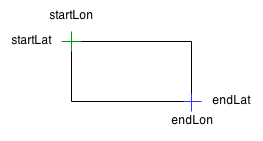
\includegraphics[height=3cm]{img/REST_boundary.png}
	\caption{Boundary specification}
	\label{fig:rest_api_boundary}
\end{figure}

\section{Overview}

In the figure \ref{fig:rest_api_tree} you can see a tree describing REST \gls{API}. The root of the tree represents root of the application and \gls{URL}s are represented by paths from root to leaf nodes.

\begin{figure}[h]
	\centering
	
\includegraphics[height=5cm]{img/REST_API.png}
	\caption{REST API tree}
	\label{fig:rest_api_tree}
\end{figure}

\section{Examples}

\subsection{Retrieving salinity data}
\label{subsec:rest_example_salinity}
In this example we will retrieve salinity information from the area between $65.24\,^{\circ}\mathrm{N}$ $7.56\,^{\circ}\mathrm{E}$ and $65.42\,^{\circ}\mathrm{N}$ $9.542\,^{\circ}\mathrm{E}$, from the depth 2 meters and from 5.8.2013.

The final path will be \path{/feature/salinity/area} and parameters \path{startLat=65.24&startLon=7.56&endLat=65.42&endLon=9.542&depth=2&time=2013-08-05}. Resulting URI will have the form - \path{/feature/salinity/area?startLat=65.24&startLon=7.56&endLat=65.42&endLon=9.542&depth=2&time=2013-08-05}.

If everything goes well, we will receieve image describing requested information as shown in figure \ref{fig:rest_example_1}.

\begin{figure}[h]
	\centering
	
\includegraphics{img/REST_example_1.png}
	\caption{Salinity in requested area}
	\label{fig:rest_example_1}
\end{figure}

\subsection{Missing compulsory parameters}
In this example we will try to retrieve depth information, but won't specify any parameters.

\begin{description}
	\item[Request] \path{/feature/depth/area}
	\item[Response] ~\\
		\begin{description}
			\item[\gls{HTTP} status] \texttt{400 Bad Request}
			\item[\gls{JSON} body] \texttt{\{"errorMessage":} \texttt{"Missing~query~parameters~in~url.",} \texttt{"error":} \texttt{\{"missingFields":} \texttt{["startLat","startLon","endLat","endLon"]\}\}}
		\end{description}
\end{description}

\subsection{Missing source file}
In this example we will request temperature data from missing file. We will use the same parameters as in first example (\ref{subsec:rest_example_salinity}).

\begin{description}
	\item[Request] \path{/feature/temperature/area?startLat=65.24&startLon=7.56&endLat=65.42&endLon=9.542&depth=2&time=2013-08-05}
	\item[Response] ~\\
		\begin{description}
			\item[\gls{HTTP} status] \texttt{500 Server Error}
			\item[\gls{JSON} body] \texttt{\{"errorMessage":} \texttt{"Could not read data file.",} \texttt{"cause":} \texttt{"/home/ondra/School/NTNU/TDT4290/netcdf/samples\_2013.08.05.nc (No such file or directory)"\}}
		\end{description}
\end{description}

\chapter{Building and Deploying}
\section{Building the project}
The project has a number of dependencies that need to be present on the target system in order to build:
Java SE Developer kit 8 \footnote{http://www.oracle.com/technetwork/java/javase/downloads/jdk8-downloads-2133151.html} (or later)
Maven 3.2.2 \footnote{http://maven.apache.org/download.cgi} (or later)
Git \footnote{http://git-scm.com/} (or later).

With these dependencies installed on the target system, your are ready to build the project.
This guide assumes you are on a *NIX system. For a windows-based system, the steps are similar but not necessarily the same. It should however be obvious to an experienced Windows user how the steps should be executed on her system.

To clonse and build the program:
\begin{lstlisting}
$ git clone git@github.com:kproj6/featureserver.git && cd featureserver
$ mvn clean package
\end{lstlisting}

To run the program locally:
\begin{lstlisting}
$ java -jar target/featureserver-0.1-SNAPSHOT-jar-with-dependencies.jar --netcdf-file={full/path/to/data/NetCdfFile.nc} --webserver-port=10100
\end{lstlisting}

This starts up the program on port 10100. The port flag defaults to 10100, so can be omitted unless you want to run on a different port.

\section{Deployment}
To deploy the program to a server, you need to first clone the repository to the server, as described above.
This guide assumes the project is cloned to the user's home directory on the server.

We have created a deploy-script which is in the root folder of the code repository:
\begin{lstlisting}
	#!/bin/sh
	# This script will ssh into the server, fetch the latest commits from github, build the program, stop the old process and start a new one.
	USER=featureserver
	SERVER_IP=178.62.233.73
	ssh $USER@$SERVER_IP '
	    cd ~/featureserver
	    git fetch
	    git reset --hard origin/master
	    mvn clean package
	    ./svc.sh stop
	    ./svc.sh start
	'
\end{lstlisting}

Change the USERNAME and SERVER\_IP variables according to your server setup, then run the script to automatically redeploy the server with the newest changes.

This script calls another script which lies on the server, the service wrapper script (svc.sh).
The service wrapper script simply makes sure that the program keeps running after the user has logged off the server. It can be used to start and stop the server manually if required.

\chapter{Templates}
In the \gls{course compendium}, the team is asked to create templates for internal documents. The team identified 3 types of documents they would need templates for:

\begin{itemize}
\item Weekly status report
\item Agenda
\item Minutes from meetings
\end{itemize}

Attached below are the templates for these documents. The minutes and agenda documents can be used both for customer meetings, advisor meetings and internal meetings.

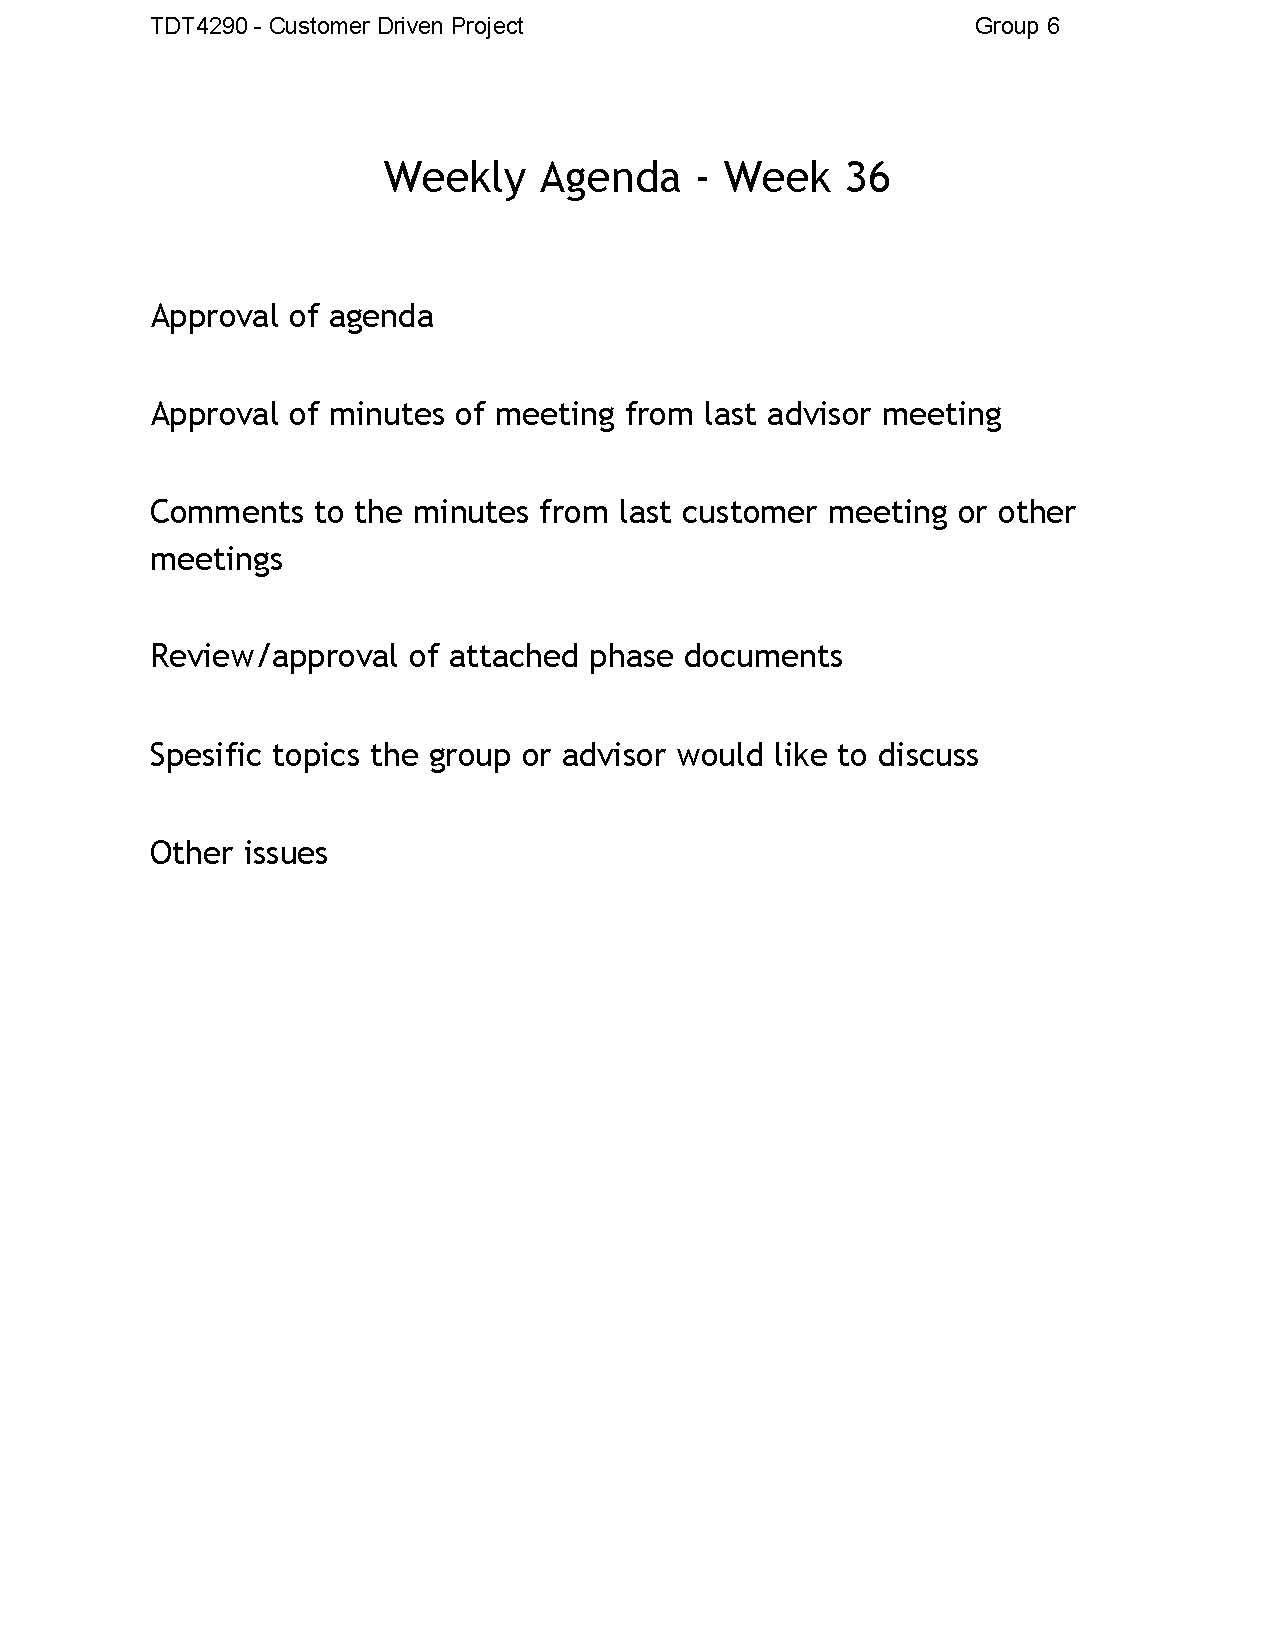
\includepdf[pages={1}]{pdf/Agenda.pdf}
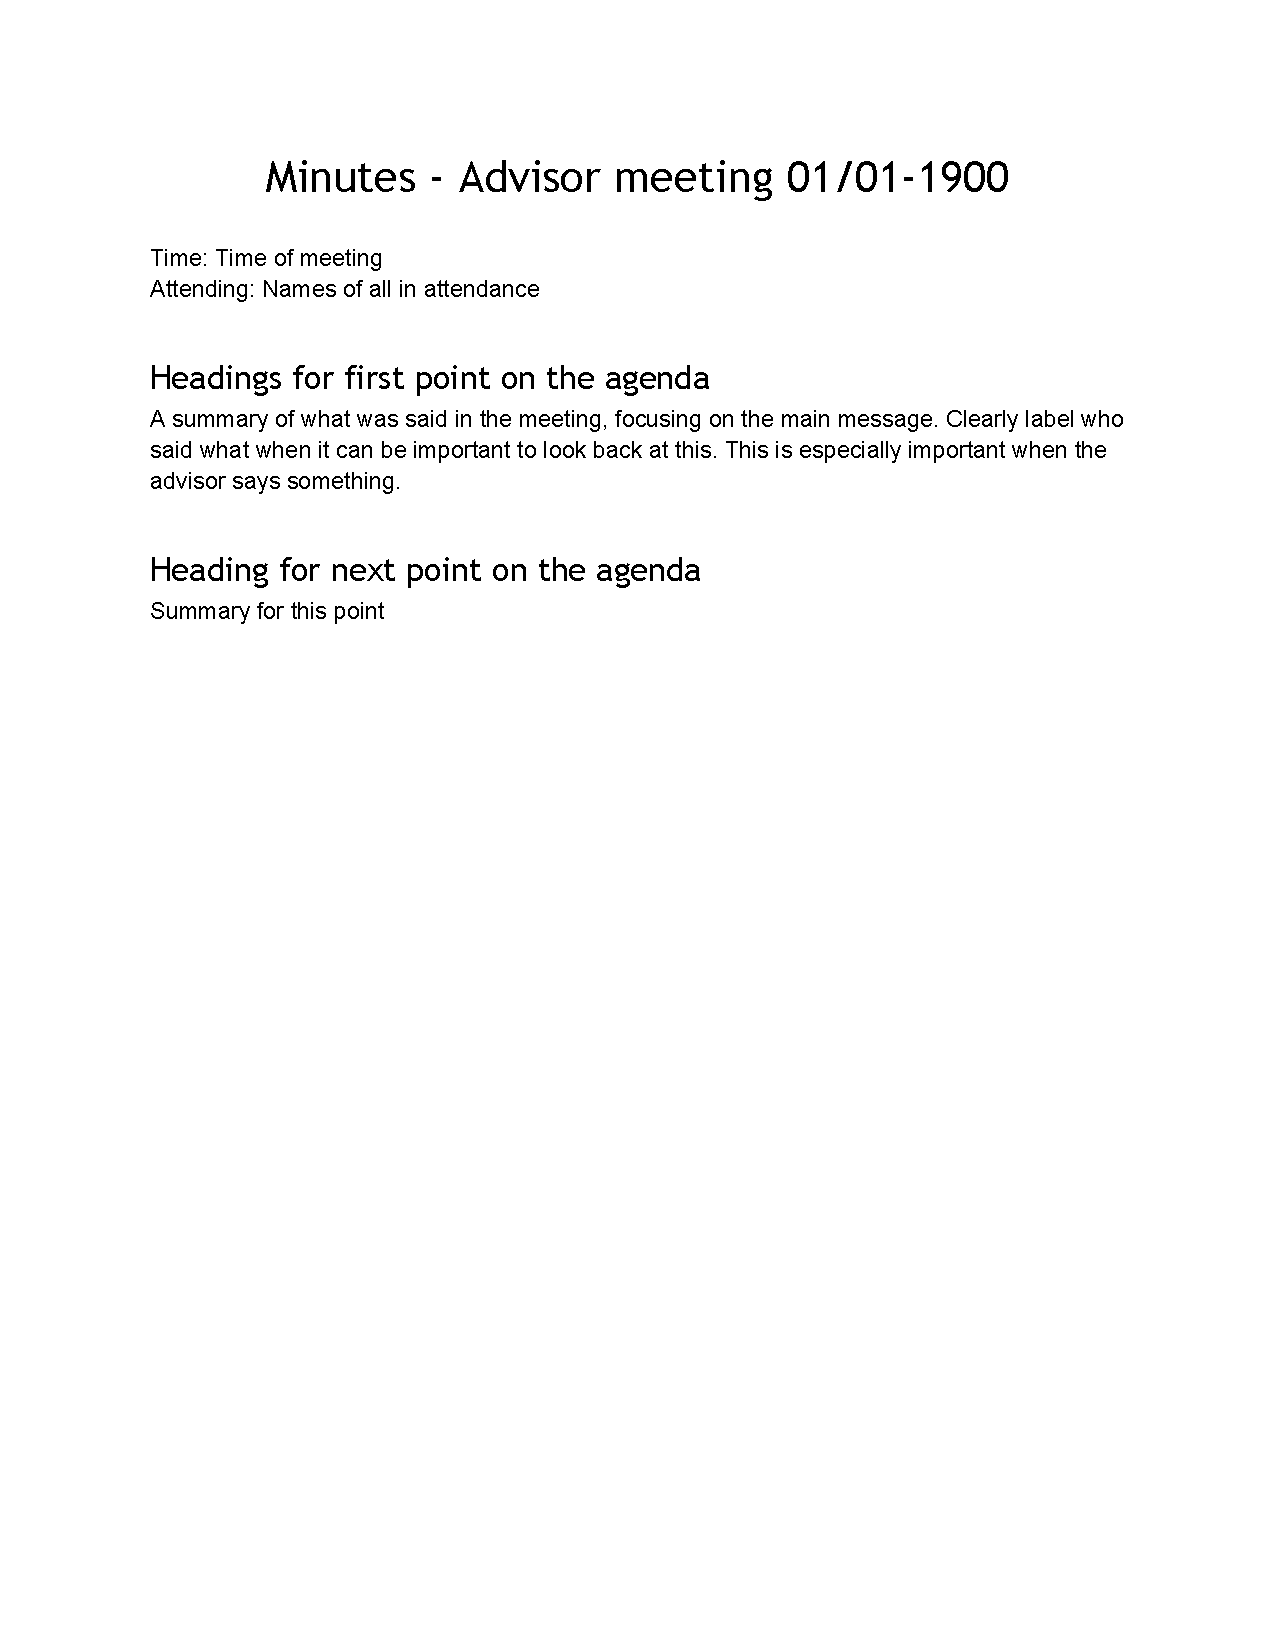
\includepdf[pages={1}]{pdf/Minutes.pdf}
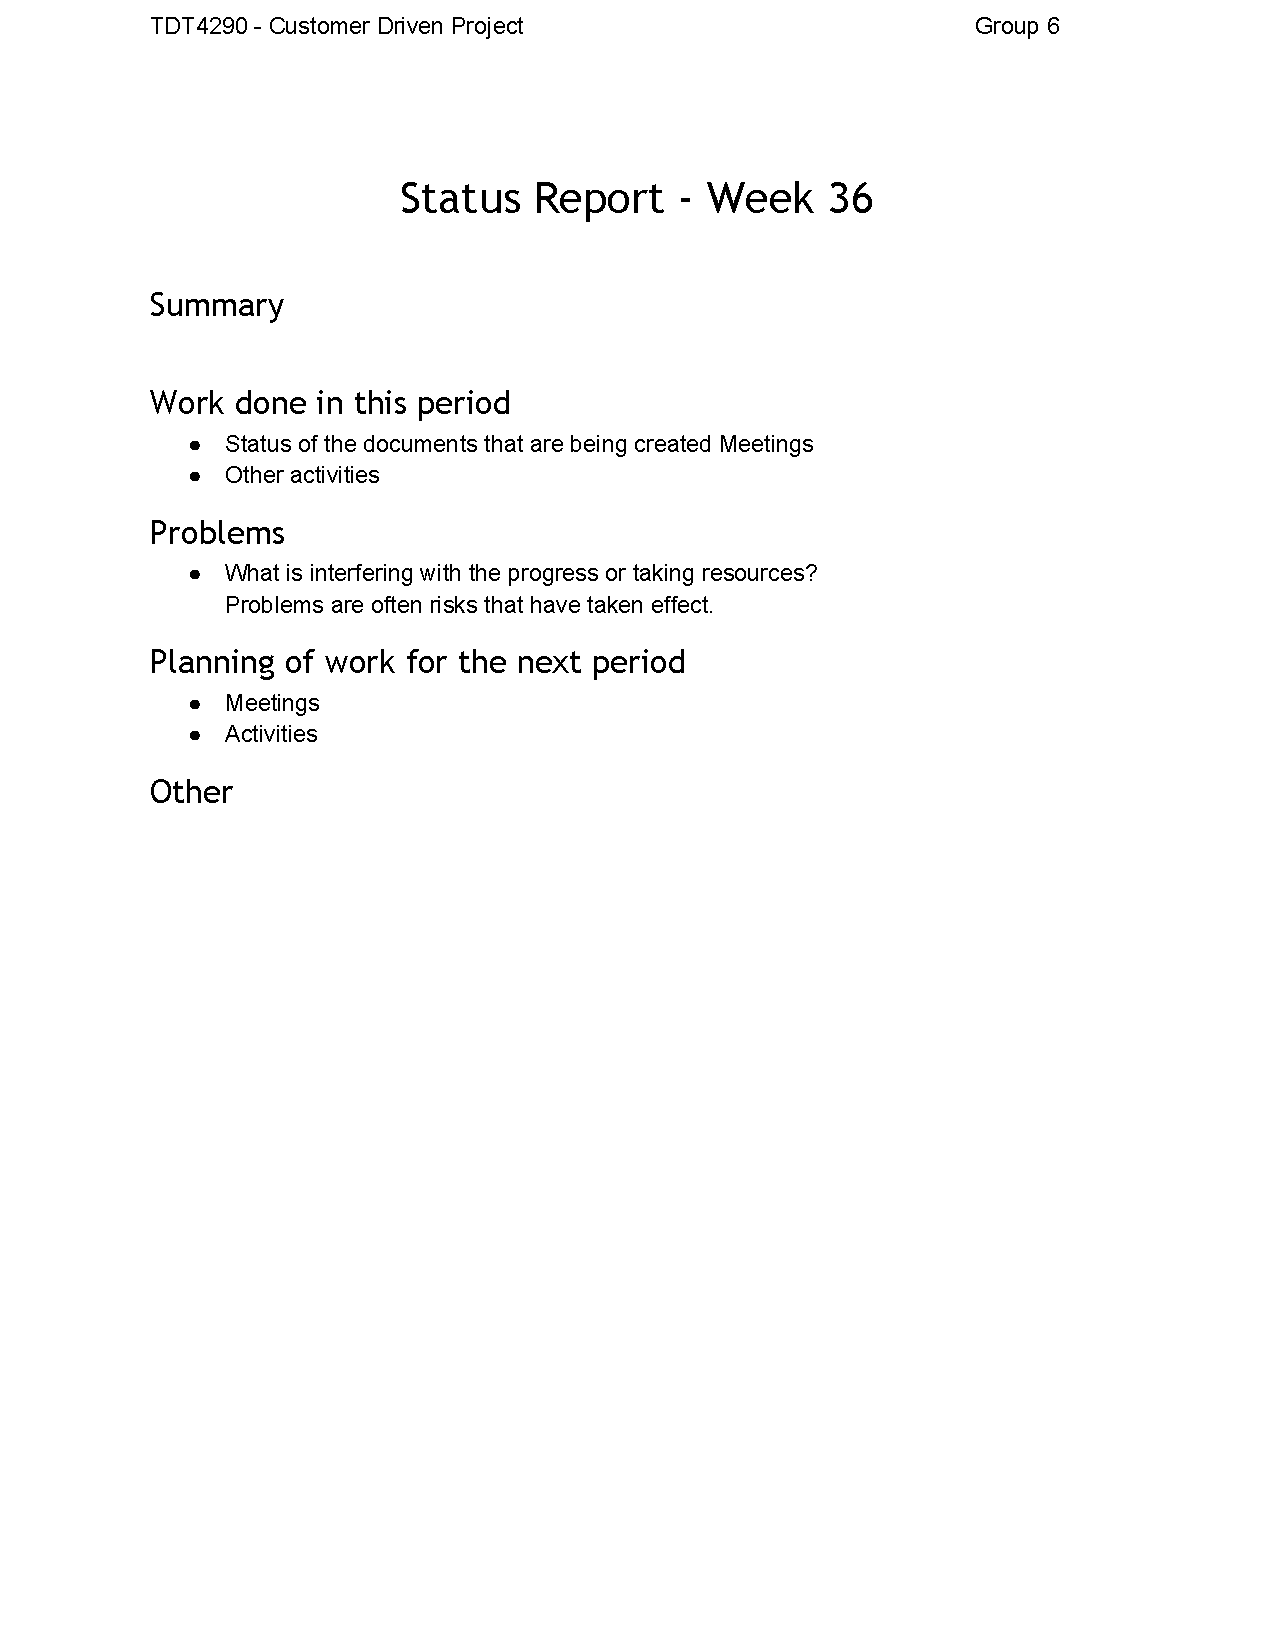
\includepdf[pages={1}]{pdf/Statusreport.pdf}

\end{document}
